\chapter{\gkchapter{Tête et dépendance}{Hiérarchiser la structure syntaxique}}\label{sec:3.3}

\section{Hiérarchie}\label{sec:3.3.0}

Les syntaxèmes, mots et autres unités syntaxiques ne sont pas seulement connectés les uns aux autres : certains dominent les autres et leur imposent leurs propriétés syntaxiques (catégorie, forme, fonction, place). Nous avons largement argumenté l’existence d’une structure syntaxique hiérarchique lorsque nous avons étudié les exemples \textit{Pierre a été malade pendant deux semaines} et \textit{La maladie de Pierre a duré deux semaines} dans le \chapref{sec:1.2}. Nous renvoyons le lecteur à cette discussion. De nouveaux éléments seront donnés dans la suite de ce chapitre. En particulier :

\begin{itemize}
\item les contraintes distributionnelles ;
\item la rection ;
\item la hiérarchie sémantique ;
\item les contraintes sur l’ordre des mots.
\end{itemize}

Avant cela, nous allons introduire un peu de terminologie, en nous basant sur la notion de connexion, introduite au chapitre précédent.

\section{Tête et dépendance}\label{sec:3.3.1}

La hiérarchie de la structure syntaxique se traduit par une asymétrie des combinaisons entre unités, lesquelles combinent alors une unité hiérarchiquement supérieure à une unité qui lui est assujettie.

\Definition{\textstyleTermes{dépendance}}
{Une \hi{connexion hiérarchisée} est appelée une \textstyleTermes{dépendance}.}

\Definition{\textstyleTermes{gouverneur}, \textstyleTermes{dépendant}}
{Si A et B sont connectés et que A est hiérarchiquement supérieur à B, on dit que A \textstyleTermes{gouverne} B et que B \textstyleTermes{dépend} de A. Ou encore que A est le \textstyleTermes{gouverneur} de B et que B est un \textstyleTermes{dépendant} de A. En général, un élément peut avoir un nombre quelconque de dépendants, mais il n’a qu’un seul gouverneur.}

En syntaxe de dépendance, depuis les travaux fondateurs de Lucien Tesnière, les dépendances syntaxiques lient des mots entre eux. Dans notre approche, les dépendances, comme les connexions, peuvent être considérées entre n’importe quelles unités syntaxiques et une même dépendance peut être décrite de façon plus ou moins fine en l’attribuant à des unités syntaxiques plus ou moins larges (voir la \sectref{sec:3.2.14} sur \textit{La connexion et ses instances}). Nous manipulerons des structures de granularité variable : parfois les mots seront les nœuds de la structure, mais parfois nous considérerons des unités plus fines (les syntaxèmes) ou des unités plus larges (voir la \sectref{sec:3.2.18} sur \textit{Structures de connexion, granularité et critères} et la \sectref{sec:3.4.1} sur l’\textit{Arbre de Beauzée-Gladkij}).

Une dépendance est représentée par une \hi{flèche} qui va \hi{du gouverneur vers le dépendant} ou encore simplement en positionnant le \hi{gouverneur au dessus du dépendant}. Nous illustrons cela avec l’énoncé \textit{Marie parle} où le verbe \textit{parle} gouverne \textit{Marie}.

\begin{figure}
%%[Warning: Draw object ignored]
\begin{tikzpicture} [every node/.style={font=\strut}]
  \matrix [row sep=1em, column sep=.75em] (matrix)
    {
      \node (parle) [ConcSet] {parle}; & \node {gouverneur};\\
      \node (Marie) [ConcSet] {Marie}; & \node {dépendant};\\
    };
  \draw (parle) -- (Marie);
\end{tikzpicture}\hspace{2cm}
\begin{tikzpicture}[every node/.style={font=\strut}]
  \matrix [row sep=.5em, column sep=1em] (matrix)
    {
      \node (Marie) [ConcSet] {Marie}; & \node (parle) [ConcSet] {parle};\\
       \node {dépendant}; & \node {gouverneur};\\
    };
\draw[-{Triangle[]}] (parle) to [bend right] (Marie);
\end{tikzpicture}
\caption{\label{fig:}Deux représentations d’une dépendance}
\end{figure}

Le sens de la flèche, du gouverneur vers le dépendant, est une convention. Comme toute convention, elle est en partie arbitraire. Il aurait été tout à fait possible d’orienter les flèches dans l’autre sens, comme certains auteurs l’ont fait. Nous adoptons ici la convention qui est la plus largement répandue.

La représentation avec le gouverneur au dessus est également arbitraire, même si l’on est largement habitué aujourd’hui à une telle représentation de la hiérarchie (voir par exemple l’organigramme des responsabilités dans une entreprise). Dans ses premiers schémas en \citeyear{tesniere1934comment}, Tesnière adoptait une autre convention : il plaçait l’élément dominant au centre comme le soleil au centre du système solaire (voir l’\encadref{sec:3.3.5} sur l’\textit{Historique des représentations syntaxique par des diagrammes en dépendance}).

Nous allons introduire un autre terme à ne pas confondre avec \textit{gouverneur}.

\Definition{\textstyleTermes{tête d'une unité syntaxique}}
{On appelle \textstyleTermes{tête} d’une unité syntaxique U toute sous-unité de U qui n’est gouvernée par aucune autre sous-unité de U.}

Les notions de tête et de gouverneur renvoient au même concept, mais adopte des points de vue différents.

\Definition{\textstyleTermes{dépendant}, \textstyleTermes{gouverneur}}
{Si A et B forment à eux deux une unité syntaxique dont A est la \hi{tête}, alors A est le \textstyleTermes{gouverneur} B. Inversement, si A est le \textstyleTermes{gouverneur} B, alors A et B forment une unité syntaxique ensemble et A en est la \hi{tête}. Enfin, B est le \textstyleTermes{dépendant} de A si et seulement si A est le \textstyleTermes{gouverneur} B.}

Autrement dit, hiérarchiser une connexion revient donc à décider de quel côté est sa tête.

On aura noté que pour une unité syntaxique U donnée, \hi{la tête de} U \hi{est un élément de} U, en quelque sorte l’élément le plus important de U du point de vue de la syntaxe, tandis que \hi{le gouverneur de} U \hi{est un élément extérieur à} U. (On peut se souvenir, pour ne pas confondre les deux termes, que la tête d’une personne fait toujours partie de cette personne.) Illustrons ces notions avec \textit{une très jolie valise} et U = \textit{très jolie}. La tête de U est \textit{jolie}, tandis que le gouverneur de U est \textit{valise}.

\begin{figure}
\begin{tikzpicture}[every pin edge/.style={dashed,lsDOIGray}]
\node at (0,0) [ConcSet,pin=west:{gouverneur de U}] (valise) {valise};
\node at (0,-2) [ConcSet,pin=east:{tête de U}] (jolie) {jolie};
\node at (0,-4) [ConcSet] (tres) {très};
\draw (valise) -- (jolie) -- (tres);
\node [fit=(tres) (jolie), draw, ellipse, inner sep=0pt,pin=west:U] {};
\end{tikzpicture}
  \caption{\label{fig:}Gouverneur vs. tête}
\end{figure}

Les grammaires de dépendance traditionnelles font l’hypothèse que toute unité possède un unique mot tête. Nous considérons pour notre part que la nature de la tête dépend de la granularité de l’analyse et qu’on peut considérer, selon les finalités de l’analyse, une unité plus fine que le mot (un syntaxème) comme une unité plus large. Par ailleurs, il peut arriver que plusieurs éléments possèdent des propriétés de tête : on parle alors de \textstyleTermes{co-têtes} (voir la \sectref{sec:3.3.27} sur \textit{Nom et déterminant comme co-têtes}).

Concluons cette section en soulignant une propriété fondamentale que nous exploiterons pour identifier la tête d’une unité : le \hi{gouverneur} d’une unité U est \hi{connecté à la tête} de U.

\chevalier[sec:3.3.2]{Historique des notions de dépendance et de tête}{%
    Le premier grammairien à utiliser le terme «~dépendance~» dans un sens grammatical est semble-t-il un grammairien arabe, \hi{Ibn Mada}, qui vécut en Espagne (alors sous domination arabe) entre 1119 et 1195. Il est connu pour son livre, intitulé \textit{La réfutation des grammairiens}, dans lequel il s’attaque à des sujets qui sont toujours d’actualité. Il critique l’utilisation de formes invisibles sous-jacentes et notamment l’introduction d’un morphème zéro pour le nominatif. Il se prononce aussi en faveur d’une indépendance de la syntaxe et de la sémantique et contre une justification sémantique ou une interprétation cognitive des règles grammaticales : «~Et pourquoi l’agent est-il au nominatif ? La réponse correcte est […] que c’est ainsi que parlent les Arabes.~» Comme nous l’avons dit, il utilise le terme {\arfont تعلق} \textit{ta’alluq}, qui se traduit par \textit{être accroché à, dépendre de, être connecté à, joindre, attachement, amour du monde, dépendance, connexion, relation,} et même \textit{obsession.} Il préfère ce terme à {\arfont عمل} \textit{\textsuperscript{c}}\textit{amal} ‘opération, gouverner’, le terme utilisé communément à son époque en grammaire pour décrire des relations entre le gouverneur et le dépendant. Selon Ibn Mada, le gouverneur n’opère pas sur ses dépendants, il y a seulement une relation, une dépendance. Il va même jusqu’à appeler hérétique toute utilisation de \textit{\textsuperscript{c}}\textit{amal} car, selon lui, des mots ne peuvent agir sur d’autres mots et déclencher une flexion. Comme l’utilisation de \textit{ta’alluq} était essentiellement un changement terminologique pour une notion établie de longue date sous le terme de \textit{\textsuperscript{c}}\textit{amal}, le terme de \textit{dépendance} n’a pas vraiment pris avant le 20\textsuperscript{e} siècle et les travaux de Lucien Tesnière, qui lui donnaient une assise théorique forte (bien que Tesnière lui-même utilise le terme de connexion).

    L’importance d’une analyse de type dépendentiel pour la description de phénomènes grammaticaux, par contre, était établie bien avant Ibn Mada. On attribue généralement à \hi{Sibawayh}, le grand grammairien perse travaillant sur l’arabe, la première modélisation grammaticale en termes de dépendances entre mots et notamment en ce qui concerne l’attribution des cas aux noms dépendant d’un verbe. Sibawayh a vécu de 760 à 796 et on raconte qu’il est mort, très jeune, de la fureur qui l’a saisi lors d’un débat sur la grammaire de l’arabe (premier accident de travail d’un linguiste~{\CryingSmiley}). Il est le fondateur d’une tradition grammaticale qui reste aujourd’hui vivace.

    Avant l’avènement de la tradition grammaticale arabe, on analysait déjà la structure des phrases en faisant référence à des liens hiérarchisés entre les mots. La plus vieille grammaire étendue qu’on connaît, les descriptions du sanskrit par l’immense linguiste indien \hi{Pāṇini} au 4\textsuperscript{e} siècle avant notre ère, introduit la notion de \textit{karaka} pour désigner les relations entre verbes et noms, qui sont classées en six classes différentes en se basant sur des critères sémantiques autant que syntaxiques. Parmi ces classes de liens, on trouve déjà l’agent/sujet (\textit{karta}) et le patient/objet (\textit{karma}). Il faudra de toute façon attendre le 20\textsuperscript{e} siècle pour une distinction claire entre les notions syntaxiques de \textit{sujet} et \textit{objet} d’une part et les notions sémantiques d’\textit{agent} et de \textit{patient} d’autre part (voir l’encadré sur \textit{Sujet, agent, thème} au \chapfuturef{18}).

    Généralement, on constate qu’une analyse en termes de dépendances s’est imposée pour pratiquement toute analyse grammaticale jusqu’à l’apparition des grammaires de constituants au 20\textsuperscript{e} siècle, en particulier pour des langues flexionnelles et à ordre libre, comme le sanskrit, l’arabe ou encore l’allemand.

    L’idée d’une analyse syntaxique complète d’un énoncé apparaît, à notre connaissance au début du 18\textsuperscript{e} siècle, en France. Il est probable que l’impulsion donnée au 17\textsuperscript{e} siècle par la parution de la \textit{Grammaire de} \hi{\textit{Port-Royal}} (\citealt{ArnauldLancelot1660}), puis de la \textit{Logique de Port Royal} (\citealt{ArnauldNicole1662}) a été déterminante. En \citeyear{buffier1709grammaire} paraît la \textit{Grammaire françoise sur un plan nouveau} de \hi{Claude Buffier} qui comprend plusieurs analyses très élaborées. Malgré le caractère très moderne de ses analyses, Buffier reste relativement peu connu, probablement en raison d’une terminologie qui ne distingue pas clairement les relations syntaxiques de la morphologie. Si l’on remplace, dans les citations qui suivent, \textit{régime} par \textit{complément} ou \textit{dépendant}, on voit que les analyses de Buffier sont de parfaites analyses en dépendance :
    \begin{quote}
      «~Tous les noms ou même tous les mots qui servent ainsi à particulariser la signification d’un autre mot, sont le régime de ce mot : comme si je dis \textit{un ami de plaisir}, la signification d’\textit{un ami} est particularisée par le mot \textit{de plaisir~}; c’est pourquoi \textit{de plaisir} est le régime d’\textit{un ami}. » (p. 57) « \textit{Dieu agit avec justice. Avec} est un mot qui n’a point de sens déterminé et complet par lui-même ; mais par le mot \textit{justice} dont il est ici suivi et qui en est le régime.~» (p. 73) 
    \end{quote}
  Les analyses de Buffier, comme celles qui suivront tout au long du 18\textsuperscript{e} siècle, sont données de manière discursive (c’est-à-dire sans schéma), ce qui les rend plus difficiles à saisir. Nous nous proposons d’en étudier une en détail dans l'exercice 1 à la fin de ce chapitre.

    Dans son ouvrage de \citeyear{girad1747vrais}, \textit{Les Vrais principes de la langue françoise, ou la Parole réduite en méthode}, l’abbé \hi{Gabriel Girard} utilise le terme \textit{dépendance} dans un sens compatible avec la définition moderne :
    \begin{quote}
    «~J’abandonne toutes les observations qu’on pourrait faire sur le Style, pour me borner uniquement à ce qui regarde l’union grammaticale des mots. Cette sorte d’union établit entre eux un RÉGIME, qui est très distingué de ce que je viens de nommer style ; ce dernier consistant dans des rapports de convenance [= relation d’accord] dont le goût fait choix pour la conduite du discours, et l’autre dans des rapports de dépendance soumis aux règles pour la construction de la phrase.~» (p. 87, nous modernisons l’orthographe) Mais Girard préfère néanmoins parler de régime plutôt que de dépendance : «~Le Régime n’est autre chose que le concours des mots pour les expressions d’un sens ou d’une pensée. Dans ce concours de mots il y en a qui tiennent le haut bout ; ils en régissent d’autres, c’est-à-dire qu’ils les assujettissent à certaines lois : il y en a qui se présentent d’un air soumis ; ils sont \textit{régis} ou tenus de se conformer à l’état et aux lois des autres ; et il y en a qui sans être assujettis ni assujettir d’autres, n’ont de lois à observer que celle de la place dans l’arrangement général.~» (p. 87)
    \end{quote}
  (L’idée, exprimée à la fin de cette citation, qu’il y a des mots qui n’entrent pas dans la rection, sera reprise par l’Approche pronominale et conduira à la distinction entre micro et macrosyntaxe ; voir partie 6.)

    \hi{Nicolas Beauzée}, dans l’article «~Régime~» de l’\textit{Encyclopédie} (\citeyear{Beauzée1765}), va introduire la distinction entre la notion de \textit{complément} et le régime proprement dit (c’est-à-dire «~la forme particulière que doit prendre un complément grammatical d’un mot, en conséquence du rapport particulier sous lequel il est alors envisagé~»), critiquant au passage l’emploi du terme \textit{régime} par Girard. Beauzée est ainsi le premier à distinguer clairement \hi{dépendance syntaxique} et \hi{dépendance morphologique} (voir encadré suivant). Beauzée ne dessine pas de diagramme, mais il fait une description détaillée de la structure syntaxique qui est similaire aux diagrammes que proposera Aleksej Gladkij plus de deux siècles plus tard (\citeyear{gladkij1968describing}), diagrammes que nous appellerons pour cette raison des arbres de Beauzée-Gladkij (voir \sectref{sec:3.4.1} \textit{Arbre de Beauzée-Gladkij}) : 
    \begin{quote}
   «~Par exemple, dans cette phrase, \textit{nous avons à vivre avec des hommes semblables à nous :} ce dernier \textit{nous} est le \textit{complément} de la préposition \textit{à ; à nous} est celui de l’adjectif \textit{semblables ; semblables à nous} est le \textit{complément} total du nom appellatif \textit{les hommes ; les hommes semblables à nous}, c’est la totalité du \textit{complément} de la préposition \textit{de}.~»
 \end{quote}
    Mieux encore, Beauzée distingue le \textit{complément grammatical} ou \textit{initial}, qui est un mot, du \textit{complément logique} ou \textit{total}, qui en est la projection (voir \sectref{sec:3.3.30} \textit{Dominance et projections maximales}), montrant ainsi le passage d’un arbre de Beauzée-Gladkij à un arbre de dépendance (que nous détaillerons tout au long du \chapref{sec:3.4}) : 
    \begin{quote}
    «~Par exemple, dans cette phrase, \textit{avec les soins requis dans les circonstances de cette nature ;} le mot \textit{nature} est le \textit{complément} grammatical de la préposition \textit{de : cette nature} en est le \textit{complément} logique : la préposition \textit{de} est le \textit{complément} initial du nom appellatif \textit{les circonstances ;} et \textit{de cette nature} en est le \textit{complément} total : \textit{les circonstances}, voilà le \textit{complément} grammatical de la préposition \textit{dans ;} et \textit{les circonstances de cette nature} en est le \textit{complément} logique.~»
     \end{quote}
     Il faut néanmoins remarquer que le sujet n’est pas considéré comme un dépendant du verbe, ce que souligne le choix même du terme \textit{complément} (voir la discussion dans le \chapfuturef{18}). Beauzée énonce même la \hi{projectivité} (voir la \sectref{sec:3.5.14} sur la \textit{Projectivité}), notant que les compléments logiques/totaux tendent à être continues.

    On peut considérer que Beauzée est le premier linguiste à donner une description claire d’une structure de dépendance. Cette description est faite à base de mots et ne trouve pas encore de traduction graphique, mais elle n’en reste pas moins une véritable analyse en dépendance. Cette opinion converge avec celle de Jean-Claude Chevalier, qui considère dans son monumental ouvrage de \citeyear{chevalier1968histoire} sur l’histoire de la syntaxe de 1530 à 1750 qu’avec Beauzée s’achève la définition de la notion actuelle de \hi{complément}.

    Les idées de Beauzée doivent beaucoup à celles de \hi{Dumarsais} qui rédigea onze ans plus tôt l’article «~Construction~» de l’\textit{Encyclopédie} (\citeyear{Dumarsais1754}). Dans cet article, Dumarsais décrit la dépendance en utilisant le terme \textit{détermination} : 
    \begin{quote}«~Un mot doit être suivi d’un ou de plusieurs autres mots déterminants, toutes les fois que par lui-même il ne fait qu’une partie de l’analyse d’un sens particulier ; l’esprit se trouve alors dans la nécessité d’attendre et de demander le mot déterminant, pour avoir tout le sens particulier que le premier mot ne lui annonce qu’en partie. […] Quelqu’un me dit que \textit{le Roi a donné ;} ces mots \textit{a donné} ne font qu’une partie du sens particulier, l’esprit n’est pas satisfait, il n’est qu’ému, on attend, ou l’on demande, 1° \textit{ce que le Roi a donné,} 2° \textit{à qui il a donné.} On répond, par exemple, à la première question, que \textit{le Roi a donné un régiment :} voilà l’esprit satisfait par rapport à la chose donnée ; \textit{régiment} est donc à cet égard le déterminant de \textit{a donné,} il détermine \textit{a donné.} On demande ensuite, \textit{à qui le Roi a-t-il donné ce régiment} ? on répond \textit{à monsieur N.} ainsi la préposition \textit{à}, suivie du nom qui la détermine, fait un sens partiel qui est le déterminant de \textit{a donné}.~» 
     \end{quote}
     (Voir l'exercice 2 pour une autre analyse de Dumarsais.)

    Sans que le terme \textit{complément} ne soit utilisé de façon aussi systématique, Dumarsais ébauche la distinction entre complément grammatical et complément logique qui sera ensuite élaborée par Beauzée et qui préfigure la distinction actuelle entre une analyse en dépendance et une analyse en constituants : 
    \begin{quote}«~On peut considérer une proposition ou grammaticalement ou logiquement : quand on considère une proposition grammaticalement, on n’a égard qu’aux rapports réciproques qui sont entre les mots ; au lieu que dans la proposition logique, on n’a égard qu’au sens total qui résulte de l’assemblage des mots.~» \end{quote}

    Enfin, on doit également à Dumarsais, l’idée reprise par Tesnière (voir la \sectref{sec:3.2.8} sur la \textit{Connexion}) que le sens naît des \hi{connexions} entre les mots : 
    \begin{quote}«~Il faut d’abord établir comme un principe certain, que les mots n’ont entre eux de rapport grammatical, que pour concourir à former un sens dans la même proposition, et selon la construction pleine ; car enfin les terminaisons des mots et les autres signes que la Grammaire a trouvés établis en chaque langue, ne sont que des signes du rapport que l’esprit conçoit entre les mots, selon le sens particulier qu’on veut lui faire exprimer. Or dès que l’ensemble des mots énonce un sens, il fait une proposition ou une énonciation. Ainsi celui qui veut faire entendre la raison grammaticale de quelque phrase, doit commencer par ranger les mots selon l’ordre successif de leurs rapports, par lesquels seuls on aperçoit, après que la phrase est finie, comment chaque mot concourt à former le sens total.~» (article «~Concordance~», \textit{Encyclopédie}, \citeyear{Dumarsais1753}). \end{quote}

    L’idée d’une hiérarchie est également développée par l’abbé \hi{Roch-Amboise} \hi{Sicard}, qui dans son ouvrage de \citeyear{sicard1801elemens}, \textit{Élémens de grammaire générale appliqués à la langue française}, présente sa \hi{théorie du chiffre~}: «~On désigne certaines prépositions par le chiffre 4, et leur complément, par le chiffre 5.~» (p. 106), mais le sujet est considéré comme dominant le verbe : «~On désigne le sujet par le chiffre 1, qui est censé être l’expression d’une moitié de l‘\textit{unité}. On désigne la qualité [= l’objet] par le même chiffre, qui représente l’autre moitié de la même \textit{unité}. On désigne le mot-lien, qui est le verbe, par le chiffre 2.~» (p. 105).

    La théorie du chiffre de Sicard semble avoir été reprise par le grammairien américain \hi{James Brown}, puis par le linguiste danois \hi{Otto Jespersen}, qui en a fait une \hi{théorie des rangs}, dont le verbe est absent ! Jespersen, qui a eu une grande influence sur ses contemporains, et notamment Tesnière, écrit dans \textit{The Philosophy of Language} en \citeyear{jespersen1924philosophy} (chapitre VII) : 
    \begin{quote}«~Dans toute dénomination composite d’une chose ou d’une personne, nous voyons toujours qu’il y a un mot d’importance suprême auquel les autres sont joints ou subordonnés. Ce mot principal est défini (qualifié, modifié) par un autre mot, qui à son tour est défini (qualifié, modifié) par un troisième mot, etc. Nous sommes ainsi amenés à établir différents «~rangs~» de mots selon leurs relations mutuelles comme défini ou définissant. Dans la combinaison (\textit{un}) \textit{temps extrêmement chaud}, le mot \textit{temps}, qui est évidemment l’idée principale, peut être appelé primaire ; \textit{chaud}, qui définit \textit{temps}, secondaire ; et \textit{extrêmement}, qui définit \textit{chaud}, tertiaire.~»  \end{quote}
    Jespersen va appliquer sa théorie des rangs à une analyse formelle d’un grand nombre d’exemples dans \textit{Analytic Syntax} publié en 1937. Par exemple, \textit{It will learn it soon enough} ‘Il va apprendre ça suffisamment tôt’ est analysé S V O 3 4, indiquant ainsi que \textit{enough}\textsubscript{4} modifie \textit{soon}\textsubscript{3}.

    L’existence d’une hiérarchie s’est également exprimée à travers la notion de \hi{tête} (angl. \textit{head}), dont on peut faire remonter l’introduction au grammairien anglais \hi{Henry Sweet} (\citeyear{sweet1891new}, \textit{A new English Grammar}, sections 40 and 41) : 
    \begin{quote}«~\textbf{40}. La relation la plus générale entre des mots dans une phrase est, du point de vue logique, celle de \textbf{mot-ajout} et \textbf{mot-tête}, ou, comme on peut aussi dire, de \textbf{modifieur} et \textbf{modifié}. Ainsi dans les phrases \textit{les hommes grands ne sont pas toujours forts, tous les hommes ne sont pas forts, grand, fort} et \textit{tous} sont des mots-ajouts modifiant le sens du mot-tête \textit{hommes}. De même \textit{foncé, rapide, rapidement} sont des mots-ajouts dans \textit{rouge foncé, il a un pas rapide, il marche rapidement}. \textit{Stone} ‘pierre’ est un mot-ajout dans \textit{stone wall, wall of stone}, parce qu’il modife (défini) le sens de \textit{wall} ‘mur’. De même, \textit{book} (\textit{books}) est un mot-ajout dans \textit{book-seller} ‘marchand de livres’, \textit{bookselling, sale of books} ‘vente de livres’, \textit{he sells books} ‘il vend des livres’, \textit{he sold his books} ‘il a vendu ses livres’, les mots-têtes correspondants étant \textit{seller, selling, sells, sold}.~» Comme on peut le voir dans cette citation suivante, Sweet bascule du concept de tête à celui de gouverneur : «~\textbf{41.} […] La distinction entre mot-ajout et mot-tête est seulement relative : un même mot peut être un mot-tête dans une phrase ou un contexte et un mot-ajout dans un autre, et un même mot peut être mot-tête et mot-ajout en même temps. Ainsi dans \textit{il est très fort}, \textit{fort} est un mot-ajout de \textit{il} et en même temps mot-tête du mot-ajout \textit{très}, lequel peut lui-même être un mot-tête, comme dans \textit{il est pas très fort}.~» \end{quote}

    L’équivalence entre les notions de tête et de dépendance est formellement montrée par \hi{Yves Lecerf} dans un rapport de \citeyear{lecerf1960programme}. Cette équivalence est présentée en détail dans le \chapref{sec:3.4}.

    La première formalisation de la notion de tête revient probablement à \hi{Leonard Bloomfield}. Dans sa grande œuvre, \textit{Langage}, publiée en \citeyear{bloomfield1933language} et considérée à juste titre comme l’ouvrage fondateur de la syntaxe de constituants, Bloomfield consacre davantage d’énergie à définir la notion de tête que celle de constituant. Il y distingue notamment les \textstyleTermesapprof{constructions endocentriques} (celles qui ont une tête) des \textstyleTermesapprof{constructions exocentriques} (celles qui n’en ont pas) : 
    \begin{quote}«~Toute construction syntaxique met en jeu deux (ou parfois plus) formes libres combinées en un syntagme (\textit{phrase}), que l’on peut appeler le syntagme \textit{résultant}. Le syntagme résultant peut n’appartenir à la classe distributionnelle (\textit{form-class}) d’aucun constituant. Par exemple, \textit{John ran} n’est ni une expression nominative (comme \textit{John}), ni une expression verbale finie (comme \textit{ran}). Par conséquent, nous dirons que la construction anglaise acteur-action est \textit{exocentrique} : le syntagme résultant n’appartient à la classe distributionnelle d’aucun constituent immédiat. Inversement, le syntagme résultant peut appartenir à la même classe distributionnelle que l’un (ou plus) des constituants. Par exemple, \textit{poor John} est une expression nominale propre, comme l’est le constituant \textit{John~}; les formes \textit{John} et \textit{poor John} ont, dans l’ensemble, les mêmes fonctions. En conséquence, nous dirons que la construction anglaise caractère-substance (comme dans \textit{poor John, fresh milk}, etc.) est une construction \textit{endocentrique}.~» \end{quote} 
    On notera que la construction \textit{sujet-verbe} (appelée par Bloomfield \textit{actor-action}) est considérée comme exocentrique, une analyse qui s’est perpétuée depuis la \textit{Grammaire de Port Royal} (\citealt{ArnauldLancelot1660}) et qui va se maintenir dans les grammaires de constituants jusqu’à l’avènement de la syntaxe X-barre à la fin des années 1970 (voir \encadref{sec:3.4.19} sur la \textit{Syntaxe X-barre}).

    La «~\textstyleTermesapprof{centralité du verbe}~» et le fait que la relation sujet-verbe est exocentrique est, elle, défendue par le linguiste hongrois \hi{Sámuel Brassai} dès 1863 : 
    \begin{quote}«~Assis au début, au milieu ou à la fin de la phrase, quel que soit l’endroit où il lui plaît d’être, se trouve le verbe, relié par des liens sémantiques à ses vassaux, les dépendants. […] L’autorité du verbe n’est pas dictatoriale et ses vassaux ne sont pas des esclaves, mais ont des relations légiférées avec leur seigneur et les uns avec les autres ; ils possèdent chacun un certain degré d’autonomie et un certain rang, avec un féodalisme dont le slogan, comme aux temps historiques, est \textit{nulle terre sans seigneur} [en français dans le texte].» (d’après une traduction en anglais du hongrois dans l’article \textit{Constituency or dependency? Notes on Sámuel Brassai’s syntactic model of Hungarian} d’András \cite{imrenyi2013constituency}). \end{quote}

    \hi{Lucien Tesnière}, dès son article de \citeyear{tesniere1934comment}, défend avec véhémence la centralité du verbe : 
    \begin{quote}«~Une phrase se présente comme un système solaire. Au centre, un verbe qui commande tout l’organisme de même que le soleil est au centre du système solaire.~»\end{quote}
    Il insiste sur le fait que le sujet dépend du verbe comme les autres actants, considérant ainsi la combinaison \textit{sujet-verbe} comme endocentrique : 
    \begin{quote}«~L’opposition du sujet et du prédicat empêche ainsi de saisir l’équilibre structural de la phrase, puisqu’elle conduit à isoler comme sujet un des actants, à l’exclusion des autres, lesquels se trouvent rejetés dans le prédicat pêle-mêle avec le verbe et tous les circonstants. […] L’opposition du sujet et du prédicat masque en particulier le caractère interchangeable des actants, qui est à la base du mécanisme des voix actives et passive.~» (\citeyear{tesniere1959elements}: chapitre 49)\end{quote}
    (Le terme prédicat est à prendre ici dans un sens particulier dont nous discuterons à nouveau dans l’encadré \textit{Fonctions syntaxiques et prédicat} au \chapfuturef{18}.) Dans ses premiers diagrammes syntaxiques, Tesnière place le verbe au centre (voir \encadref{sec:3.3.5} \textit{Historique des représentations syntaxiques par des diagrammes en dépendance}).

    Premièrement, Tesnière n’a pas introduit le terme de \textit{dépendance}. Comme nous l’avons dit au chapitre précédent, Tesnière utilise le terme de {\hi{connexion}}, une connexion liant toujours pour lui un élément \hi{régissant} à un élément \hi{subordonné}. Quant à la structure qu’il associe à une phrase, il l’appelle un \textstyleTermes{stemma}. Deuxièmement, le stemma n’est pas un arbre de dépendance, mais une structure de dépendance dont certains liens ne sont pas hiérarchisés. À côté de la «~connexion~», qui est donc une dépendance chez lui, Tesnière considère deux autres types de relations syntaxiques, considérées comme exocentriques : la \hi{translation} et la \hi{jonction}. En conséquence, le stemma n’est pas non plus un graphe, puisqu’en cas de translation, le gouverneur de la translation a la translation complète pour dépendant et non l’un des éléments en relation de translation. Comme nous sommes sur des positions assez proches de Tesnière, nous aurons l’occasion de revenir sur la translation et la jonction et d’expliquer pourquoi il peut être envisagé de ne pas les considérer comme des relations hiérarchiques. La translation est discutée à la section sur \textit{La translation syntaxique} du \chapfuturef{17}. Quant à la jonction, elle fait l’objet d’un chapitre entier, le \chapfuturef{19}.

    L’idée que toutes les constructions sont endocentriques va être défendue plus tard, dans les années 1960--1970, aussi bien du côté de la syntaxe de dépendance avec l’école de Moscou (voir l’ouvrage d’\hi{Igor Mel’čuk}, \textit{Dependency Syntax}, de 1988, qui reprend des travaux publiés en russe dans les années 1960--1970), que du côté de la syntaxe de constituants avec la syntaxe X-barre (voir l’ouvrage éponyme de \hi{Ray Jackendoff} de 1977). On est ensuite revenu sur cette position en remarquant que, si l’on peut toujours se donner des critères pour attribuer une tête à chaque connexion (comme le fait Mel’čuk par exemple), il faut néanmoins reconnaître que ces critères ne s’appliquent pas de la même façon avec toutes les constructions et que dans un certain nombre de constructions un deuxième élément peut avoir des propriétés de tête. C’est la position que nous défendrons ici.

    Il faut aussi signaler que c’est seulement à partir de la fin des années 1970 que les linguistes vont répertorier de manière systématique les critères qui permettent de caractériser la tête (ou ce qui revient à peu près au même, la dépendance). On trouve des critères syntaxiques explicites pour définir la dépendance dans un article remarquable de \hi{Paul Garde} de \citeyear{garde1977ordre} (voir discussion dans l’exercice 4) et une tentative de définition systématique de la dépendance dans l’ouvrage d’\hi{Igor Mel’čuk} de \citeyear{melcuk1988dependency}. L’article d’\hi{Arnold Zwicky} de \citeyear{zwicky1985heads}, intitulé \textit{Heads}, reste fameux pour avoir répertorié les différents critères de définition de la tête et montré comment ils coïncidaient ou non selon les constructions. \hi{Richard Hudson} répond à Zwicky dans un article de \citeyear{hudson1987zwicky} en corrigeant certaines analyses et en montrant que les critères sont beaucoup plus convergents que ne le dit Zwicky.

    Nous poursuivons cette discussion dans l’\encadref{sec:3.3.5} consacré à l’\textit{Historique des représentations syntaxiques par des diagrammes en dépendance} et l’\encadref{sec:3.4.17} consacré à l’\textit{Historique des représentations syntaxiques par des diagrammes en constituants}.
}

\loupe[sec:3.3.3]{Dépendances morphologique, syntaxique et sémantique}{%
    Nous nous intéressons dans ce chapitre à la syntaxe et lorsque nous parlons de dépendance, il s’agit évidemment de \textstyleTermesapprof{dépendance syntaxique}. Igor Mel’čuk a contrasté cette notion avec celles de dépendances morphologique et sémantique.

    Les \textstyleTermesapprof{dépendances sémantiques} sont les \hi{relations prédicat-argument} qui existent entre les signifiés des sémantèmes (voir chapitres \ref{sec:1.2} et \ref{sec:2.3}). Par exemple, un verbe à l’infinitif n’a jamais de sujet, mais il possède toujours un argument sémantique qui peut être restitué par une paraphrase où le verbe est à une forme finie. Par exemple, si on compare \textit{Marie promet à Pierre de venir} et \textit{Marie permet à Pierre de venir}, dans le premier cas ‘Marie’ est l’argument de ‘venir’ (\textit{Marie promet qu’elle viendra}) et dans le deuxième cas ‘Pierre’ est l’argument de ‘venir’ (\textit{Marie permet que Pierre vienne}) (voir figure \ref{fig:promet}). Dans les deux cas, la dépendance sémantique ne correspond pas à une dépendance syntaxique, car ni \textit{Marie de venir,} ni \textit{à Pierre de venir} ne sont des unités syntaxiques. Les dépendances sémantiques seront à nouveau considérées dans le \chapfuturefici{13} sur la \textit{Syntaxe profonde}, ainsi que dans le \chapfuturef{19} où nous étudierons les distorsions entre structures syntaxique et sémantique dans les phénomènes d’extraction.
    
    \begin{figure}[H]
        \begin{minipage}{.5\textwidth}\centering
        a. {\itshape Marie promet à Pierre de venir}\\
        \begin{tikzpicture}[>={Triangle[]}]
        \graph [empty nodes, nodes={CircleNode},clockwise,n=4] 
          {
            {[nodes={label=above:{‘promettre’}}] a},
            {[nodes={label=right:{‘Pierre’}}] b},
            {[nodes={label=below:{‘venir’}}] c},
            {[nodes={label=left:{‘Marie’}}] d},
            {[edge node={node[EdgeLabel] {1}}]a -> d, c->d},
            {[edge node={node[midway,right,font=\small] {2}}]a->c},
            {[edge node={node[EdgeLabel] {3}}]a->b}
          };
        \end{tikzpicture}\end{minipage}%
        \begin{minipage}{.5\textwidth}\centering
        b. {\itshape Marie permet à Pierre de venir}\\
        \begin{tikzpicture}[>={Triangle[]}]
        \graph [empty nodes, nodes={CircleNode},clockwise,n=4] 
          {
            {[nodes={label=above:{‘permettre’}}] a},
            {[nodes={label=right:{‘Pierre’}}] b},
            {[nodes={label=below:{‘venir’}}] c},
            {[nodes={label=left:{‘Marie’}}] d},
            {[edge node={node[EdgeLabel] {1}}]a -> d, c->b},
            {[edge node={node[midway,right,font=\small] {2}}]a->c},
            {[edge node={node[EdgeLabel] {3}}]a->b}
          };
        \end{tikzpicture}
        \end{minipage}
        \caption{Représentations sémantiques}\label{fig:promet}
    \end{figure}

    Les dépendances sémantiques doivent être distinguées des \textstyleTermesapprof{relations anaphoriques}, qui lient deux éléments, généralement un pronom avec son antécédent comme \textit{la théorie du liage} et \textit{elle} dans \textbf{\textit{La théorie du liage}} \textit{soulève autant de problèmes qu’}\textbf{\textit{elle}} \textit{n’en résout}.

    On parle de \textstyleTermesapprof{dépendance morphologique} dès que le «~choix~» d’un \hi{syntaxème flexionnel} n’est pas libre, mais dépend du choix d’un autre syntaxème (voir la \sectref{sec:2.3.10} \textit{Collocation et choix liés} pour le choix non indépendant d’un lexème). Cela concerne les phénomènes d’\textstyleTermesapprof{accord} (\textit{le fauteuil est blanc}\textbf{{}-}\textrm{\textbf{${\emptyset}$}} vs \textit{la chaise est blanch}\textbf{\textit{e~}}; \textit{ce truc est génial}\textbf{{}-}\textrm{\textbf{${\emptyset}$}} vs \textit{ces trucs sont géni}\textbf{\textit{aux}}) et les \textstyleTermesapprof{régimes} (\textit{Ich sehe ein}\textbf{\textit{en}} \textit{Mann} ‘je vois un homme’ vs. \textit{Ich helfe ein}\textbf{\textit{em}} \textit{Mann} ‘j’aide un homme’, avec un complément au datif et non à l’accusatif comme précédemment et qui se traduirait littéralement par ‘j’aide \textbf{à} un homme’). Dans le cas de \textit{blanc} vs \textit{blanche}, le syntaxème flexionnel d’accord en genre sur l’adjectif \textsc{blanc} est contrôlé par le genre du nom, c’est-à-dire par le syntactique d’un lexème, alors que dans le cas de \textit{génial} vs \textit{géniaux}, le syntaxème flexionnel d’accord en nombre porté par l’adjectif \textsc{génial} est contrôlé par le syntaxème de nombre du substantif (voir néanmoins la discussion de l'\encadref{sec:3.1.16} sur les \textit{Synatxèmes discontinus}). Le régime est un syntaxème dont la présence est imposée par un gouverneur à son dépendant ; dans nos deux exemples en allemand, le verbe impose à son complément un morphème de cas (cas accusatif pour \textsc{sehen} ‘voir’ et datif pour \textsc{helfen} ‘aider’).

    On parle de dépendance morphologique seulement quand la contrainte morphologique est incontournable. Cela exclut les cas d’accord d’un pronom anaphorique lorsque la référence du pronom peut être choisie librement. Donnons un exemple :
    \ea
        \textit{\textbf{{Amélie}}  {veut rendre le livre qu’}\textbf{{elle}}  {vient d’acheter.}}
    \z
    Ici l’interprétation préférée est que \textit{elle} renvoie à \textit{Marie} et est donc au féminin parce que \textit{Marie} est féminin. Mais nous ne considérons pas cela comme une dépendance morphologique, car rien n’empêche d’avoir ici un pronom masculin (même si bien sûr le sens change) :
    \ea
        \textit{\textbf{{Amélie}}  {veut rendre le livre qu’}\textbf{{il}}  {vient d’acheter.}}
    \z
    De même que les dépendances sémantiques, les dépendances morphologiques correspondent généralement à des dépendances syntaxiques. Les régimes et les accords servent précisément à marquer des dépendances syntaxiques (voir l'\encadref{sec:1.3.3} \textit{Un exemple —} \textit{l’accord} \textit{—} \textit{de la description à l’explication}). Mais certaines dépendances morphologiques se font néanmoins à distance. Tel est le cas des accords suivants :
    \ea
        \textit{\textbf{{Amélie}}  {aimerait pouvoir rester} \textbf{{belle}}.}
    \z
    Certains considèrent qu’il n’y a pas en fait de dépendance morphologique à distance, mais que l’accord se fait localement avec un pronom zéro sujet du verbe ou de l’adjectif, lequel est \hi{localement lié} à un autre pronom et cela de manière récursive jusqu’à la source de l’accord. C’est la \textstyleTermesapprof{théorie du liage} :
    \ea
       \textit{ \textbf{{Amélie}}{\textsubscript{i}}  {aimerait} \textrm{${\varepsilon}$}{\textsubscript{i}}  {pouvoir} \textrm{${\varepsilon}$}{\textsubscript{i}}  {rester} \textrm{${\varepsilon}$}{\textsubscript{i}} \textbf{{belle}}.}
    \z
    Les pronoms zéros sont marqués par des \textrm{${\varepsilon}$} et la coréférence par la présence d’un même indice \textit{i}.

    On notera que les principes qui définissent les dépendances morphologiques et sémantiques sont également utilisés (de manière secondaire) pour définir les relations syntaxiques (voir la \sectref{sec:3.3.18} sur le \textit{Critère sémantique de non-effacement} et l’\encadref{sec:3.3.22} sur les \textit{«~Déterminants} \textit{complexes~»}), en raison de la forte coïncidence de ces notions.
}
\section{Structure de dépendance et arbre de dépendance}\label{sec:3.3.4}

Au chapitre précédent, nous avons présenté la structure de connexion, qui peut être un \hi{graphe} ou plus généralement un graphe à bulles ou un \hi{polygraphe} (voir l’\encadref{sec:3.2.23} \textit{Graphe à bulles et polygraphe}). Les connexions sont des liens syntaxiques non hiérarchisés : elles lient deux unités syntaxiques sans attribuer de rôle particulier à l’un ou l’autre.

\Definition{\textstyleTermes{structure de dépendance (partielle)}}
{Une \textstyleTermes{structure de dépendance} est une structure du même type qu’une \hi{structure de connexion}, mais dont certains liens syntaxiques sont des dépendances, c’est-à-dire des \hi{liens hiérarchisés} liant un gouverneur à un dépendant. La structure de dépendance est dite \textstyleTermes{partielle} quand au moins une connexion n’est pas hiérarchisée.}

Pour que la structure de dépendance représente une \hi{hiérarchie}, il ne suffit pas que chaque lien soit hiérarchisé. Il faut que la structure possède une autre propriété, l’\hi{acyclicité}, c’est-à-dire qu’elle ne doit contenir de cycles orientés (voir l’\encadref{sec:1.2.3} \textit{Graphe et arbre}). Autrement dit, une structure de dépendance ne contient pas de \hi{cycles de dépendances}, c’est-à-dire de boucles que l’on peut parcourir de gouverneur en dépendant pour revenir au même point. (Nous verrons une exception au \chapref{sec:5.4} lorsque nous étudierons les pronoms interrogatifs et relatifs.)

L’acyclicité n’exclut pas les cycles non orientés de connexions comme on l’a vu dans l’\encadref{sec:3.2.24} \textit{Cycle de connexions}.

\begin{figure}
\begin{subfigure}[b]{.5\textwidth}\centering
\begin{tikzpicture}[every node/.style={font=\small\strut}]
\node at (0,0) (A) [ConcSet] {Marie commet};
\node at (2,2) (B) [ConcSet] {une faute};
\node at (2,-2) (C) [ConcSet] {envers Pierre};

\draw[-{Triangle[]}] (A) -- (B);
\draw[-{Triangle[]}] (A) -- (C);
\draw[-{Triangle[]}] (B) -- (C);
\end{tikzpicture}
\caption{\textit{Marie commet une faute envers Pierre}}
\end{subfigure}%                         
\begin{subfigure}[b]{.5\textwidth}\centering
\begin{tikzpicture}[every node/.style={font=\small\strut}]
\node at (0,0) (A) [ConcSet] {la montée};
\node at (2,2) (B) [ConcSet] {du nationalisme};
\node at (2,-2) (C) [ConcSet] {en Catalogne};

\draw[-{Triangle[]}] (A) -- (B);
\draw[-{Triangle[]}] (A) -- (C);
\draw[-{Triangle[]}] (B) -- (C);
\end{tikzpicture}
\caption{\textit{la montée du nationalisme en Catalogne}}
\end{subfigure}
\caption{Cycles non orientés\label{fig:}}
\end{figure}

La présence de cycles non orientés dans une structure de dépendance entraîne que certains nœuds ont deux gouverneurs. (On parle alors de \hi{dag}, \textit{directed acyclic graph}). Dans cet ouvrage, nous ne considérerons quasiment que des structures sans cycle et pour lesquelles \hi{tout nœud} \hi{possède au plus un gouverneur}. Plus précisément, lorsque tout nœud a exactement un gouverneur (à l’exception d’un nœud qu’on appelle la racine), la structure est un arbre : l’\textstyleTermes{arbre de dépendance} (voir l'\encadref{sec:0.0.1} sur l'\textit{Arbre de dépendance}).

Notons pour conclure cette section que l’on utilise généralement une terminologie différente lorsqu’on parle d’une unité syntaxique U et de la structure S de dépendance qui lui est associée. Ainsi appelle-t-on \textstyleTermes{racine} de S le nœud de S qui correspond à la \hi{tête} de U.

\chevalier[sec:3.3.5]{Historique des représentations syntaxiques  par des diagrammes en dépendance}{%
    La première représentation dépendentielle que nous connaissons est un diagramme, unique, proposé par le philosophe et grammairien allemand Johann Billroth dans sa grammaire du latin (\textit{Lateinische Syntax}) publiée en \citeyear{Billroth1832}, à seulement 24 ans (il décédera à 28 ans).

    \begin{figure}[H]
    \caption{\label{fig:Billroth1832}Diagramme de \citet[102]{Billroth1832}}
    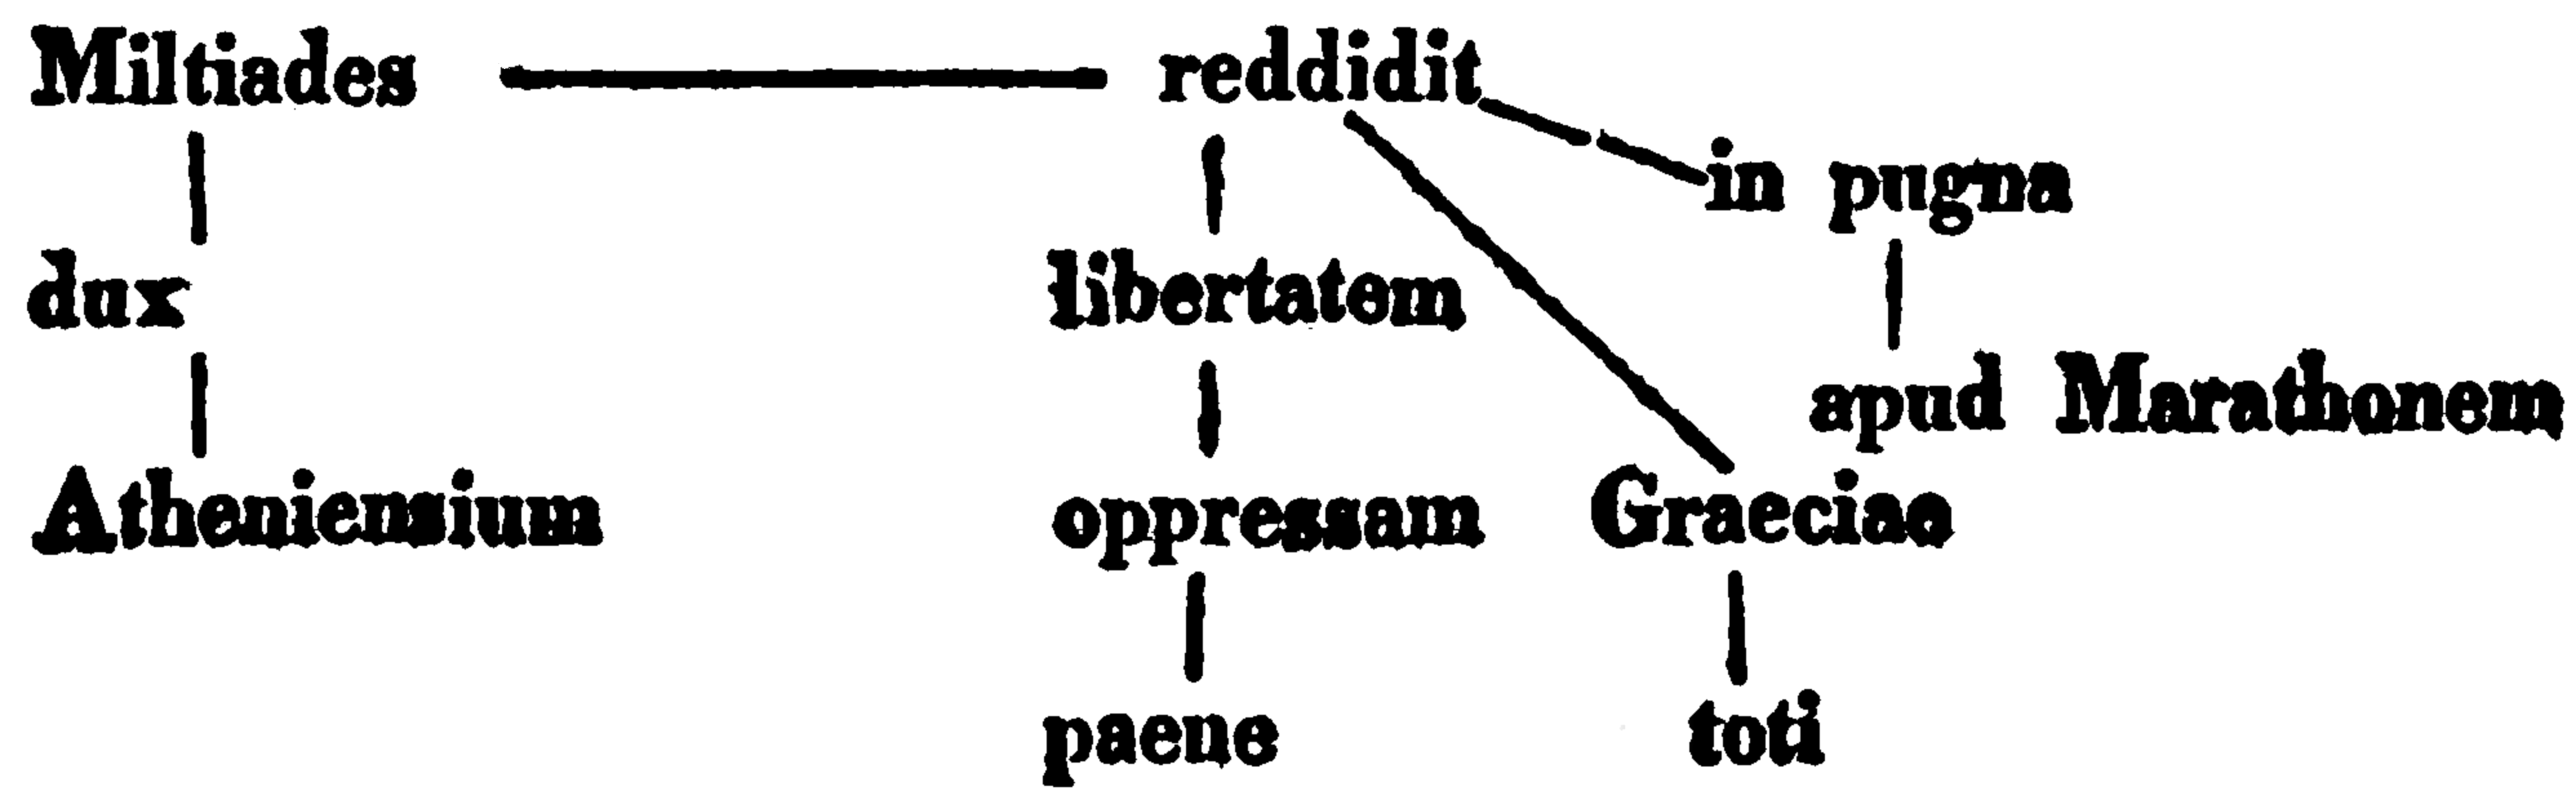
\includegraphics[width=.75\textwidth]{figures/Billroth1832.png}\smallskip\\    
    \noindent\parbox{.75\textwidth}{\small\textit{Miltiades, dux Atheniensium, toti Graeciae libertatem paene oppressam in pugna apud Marathonem reddidit.}\\
    ‘Miltiades, le chef des Athéniens, rendit à toute la Grèce la liberté dont elle avait été gravement privée en livrant bataille à Marathon.’}
    \end{figure}

    Stephen W. Clark est le premier grammairien à réellement exploiter des diagrammes dépendentiels dans sa grammaire de l’anglais de \citeyear{Clark1847} intitulé \textit{The science of the English grammar: A practical grammar in which words, phrases, and sentences are classified to their offices, and their relation to each other, illustrated by a complete system of diagrams} ‘La science de la grammaire anglaise : une grammaire pratique dans laquelle les mots, les syntagmes et les phrases sont classées selon leurs fonctions et leurs relations les uns aux autres par un système complet de diagrammes’. Dans les représentations de Clark, les connexions ne sont pas représentées en tant que telles : un mot qui en «~qualifie~» un autre (pour reprendre les termes de Clark) est placé dans une bulle sous la bulle de son gouverneur. Les prépositions comme \textit{by} ‘par’ ou \textit{of} ‘de’ dans la figure ci-dessous reçoivent une forme particulière indiquant qu’elles servent à «~connecter~» deux mots. Le sujet, le verbe et l’objet direct sont placés au même niveau, comme ici \textit{ressources} and \textit{are developed}. Les groupes prépositionnels sont entourés par des bulles en pointillés.

    \begin{figure}[H]
    \caption{\label{fig:}Diagramme de \citet[17]{Clark1847}}
    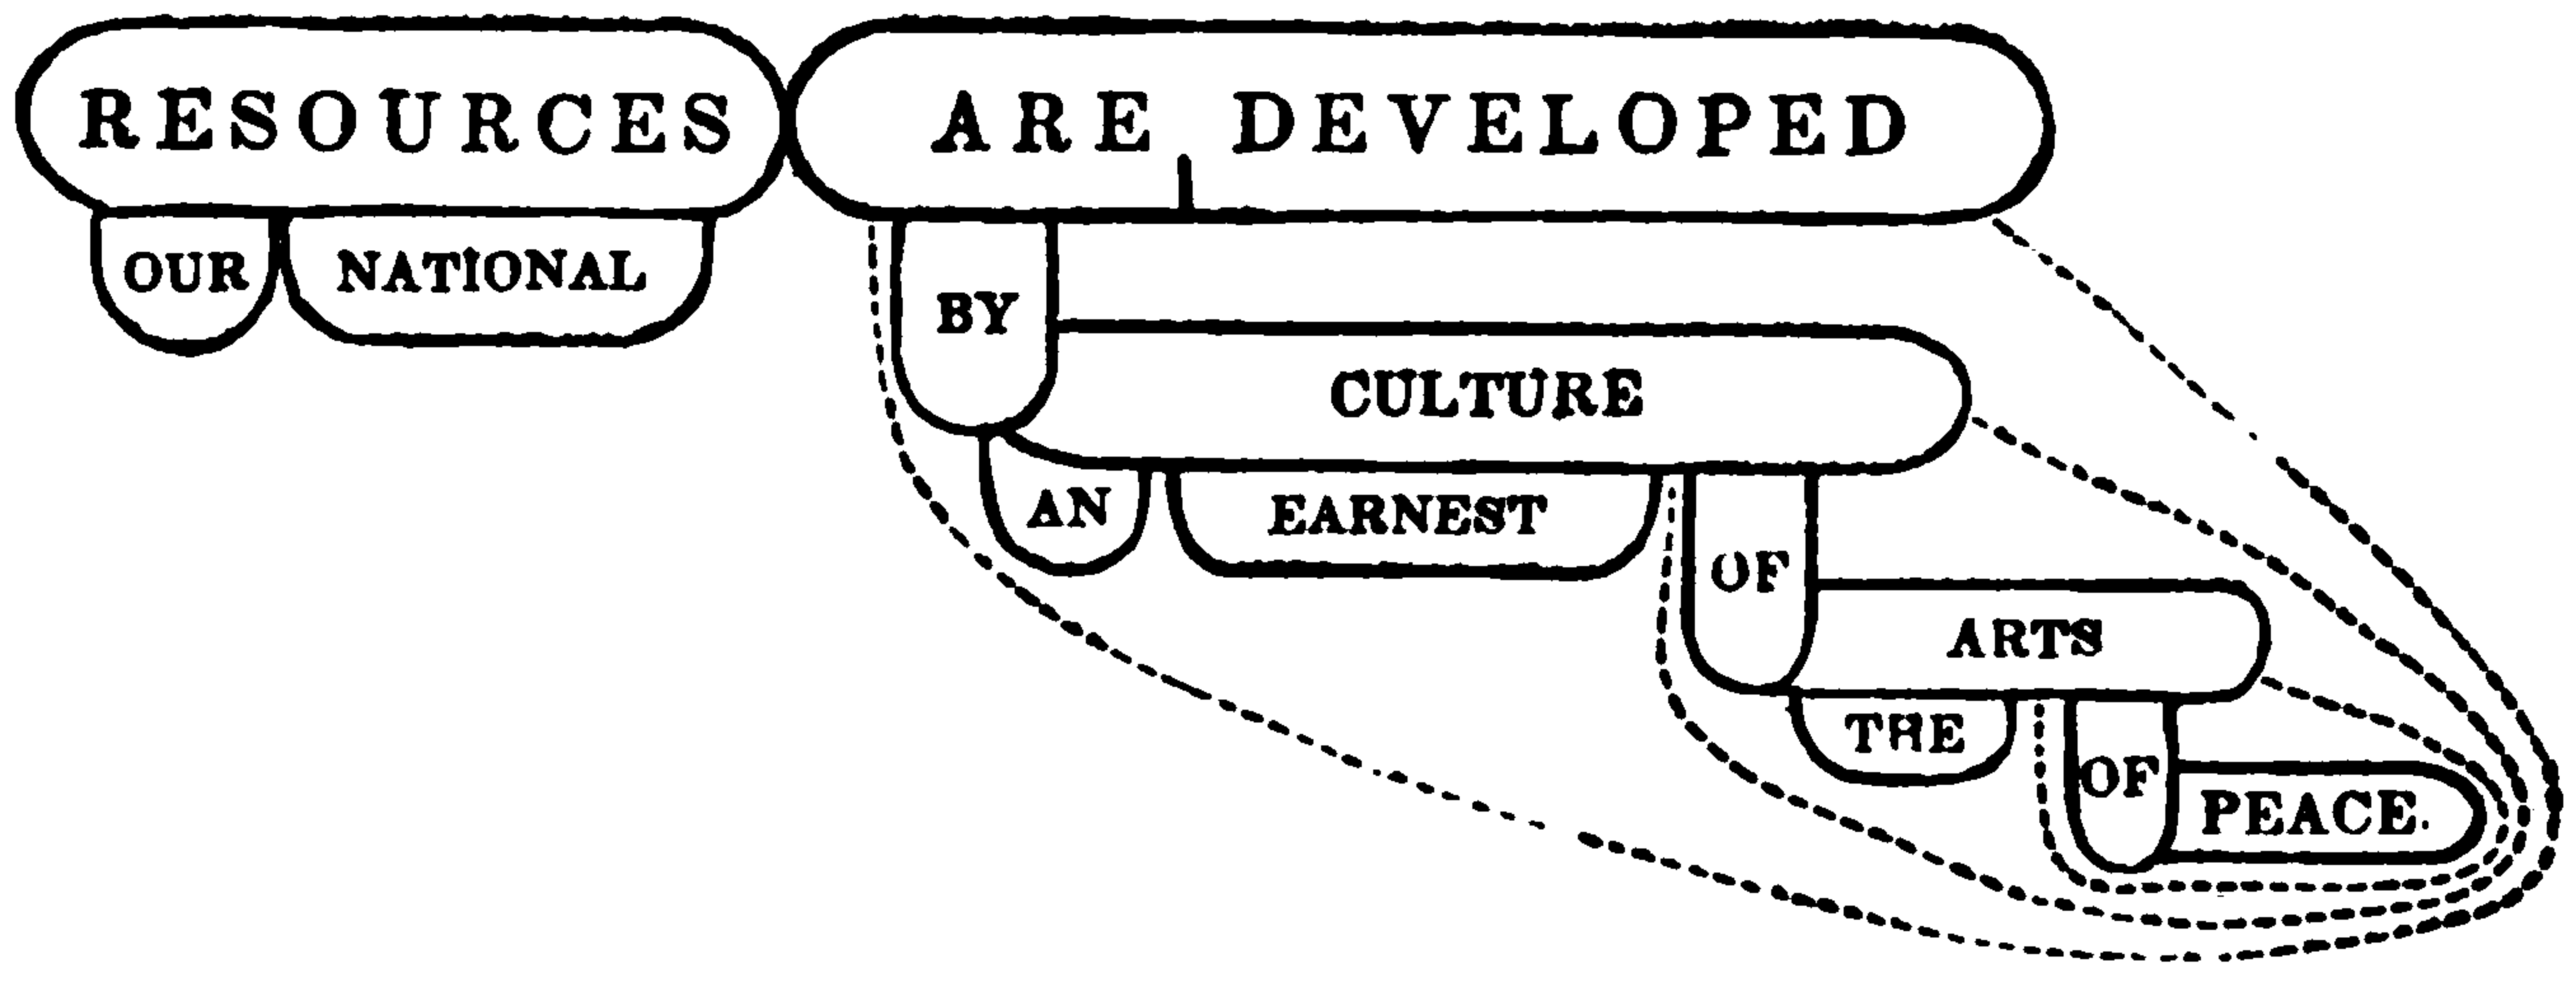
\includegraphics[width=.75\textwidth]{figures/Clark1847.png}\smallskip\\    
    \noindent\parbox{.75\textwidth}{\small\textit{Our national resources are developed by an earnest culture of the arts of peace.}\\
    ‘Nos ressources nationales sont développées grâce à une sérieuse culture des arts de la paix.’}
    \end{figure}

    Les analyses de Clark sont d’une grande cohérence et ses représentations de la coordination ou de l’extraction, sur lesquelles nous reviendrons dans le \chapfuturef{19} et le \chapfuturef{20}, sont remarquables. Il leur manque juste le développement théorique que proposera plus tard Tesnière.

    Ce ne sont pas les diagrammes de Clark qui sont passés à la postérité, mais ceux de ses suiveurs, \hi{Alonzo Reed} et \hi{Brainerd Kellogg}. Leurs diagrammes, proposés pour la première fois en \citeyear{ReedKellogg1877} et toujours utilisés aujourd’hui par certains enseignants d’anglais, sont équivalents à ceux de Clark, mais utilisent des conventions différentes : les mots ne sont plus placés dans des bulles, mais au-dessus de segments de traits. Les verbes et les noms reçoivent des segments horizontaux, comme \textit{pleased} ‘enchanté’ ou \textit{news} ‘nouvelles’ dans le diagramme qui suit, tandis que les autres mots, comme la préposition \textit{with} ‘avec’ ou l’adjectif ‘good’, reçoivent des segments en diagonal. Comme chez Clark, le sujet le verbe et l’objet sont au même niveau. Les connections apparaissent de manière plus explicite à la jointure de deux segments. La connexion entre le sujet et le verbe (\textit{girls – are pleased}) est symbolisée par un trait vertical et celle entre l’auxiliaire et le participe (\textit{are – pleased}) par un trait oblique.

    \begin{figure}[H]
    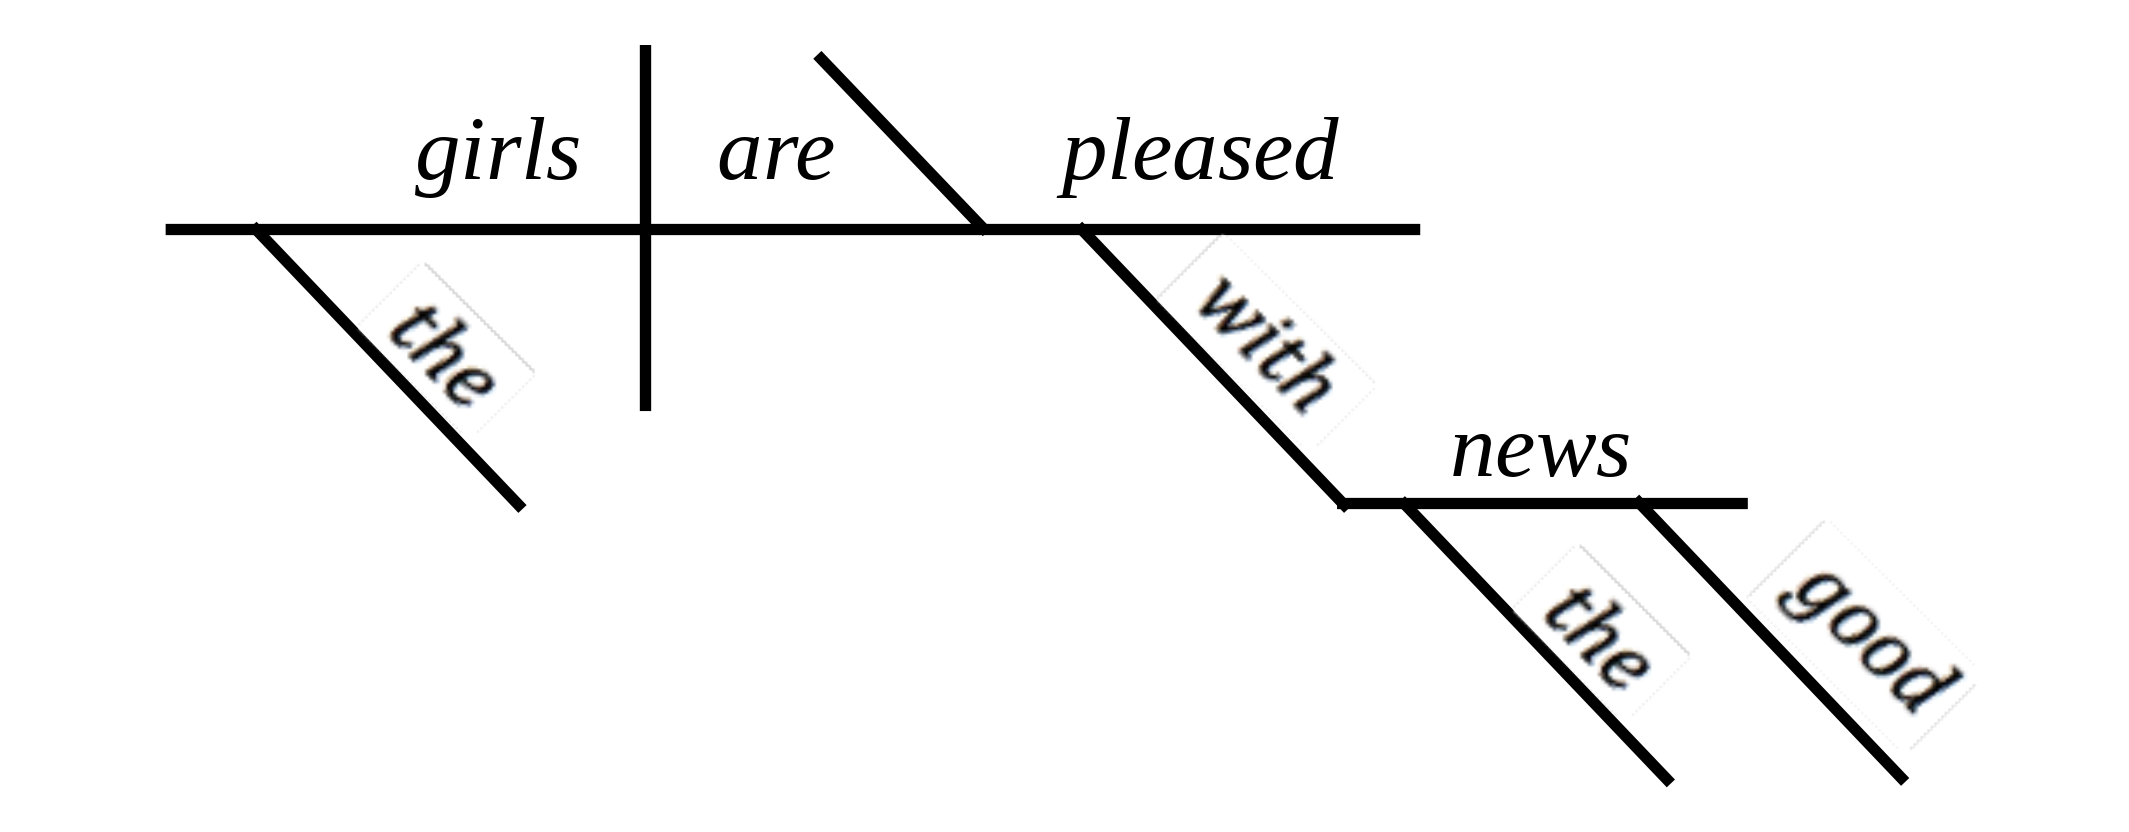
\includegraphics[width=7cm]{figures/ReedKellog}\smallskip\\    
    \noindent\parbox{7cm}{\small\textit{The girls are pleased with the good news.}\\
    ‘Les filles sont enchantées par la bonne nouvelle.’}
    \caption{Diagramme de \citet{ReedKellogg1877}}
    \end{figure}

    On peut traduire cette structure dans les conventions utilisées ici, en réifiant les connexions et en mettant en évidence le fait que certaines connexions ne sont pas hiérarchisées :

    \begin{figure}[H]
    \caption{Interprétation du diagramme de Reed \& Kellogg}
% %     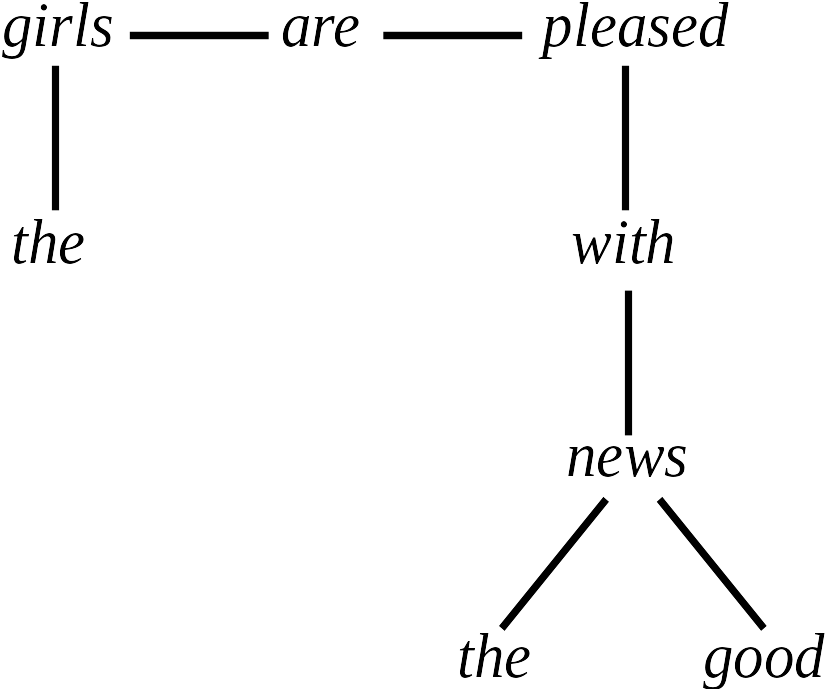
\includegraphics[width=7cm]{figures/ReedKellogTree}    
    \begin{forest} for tree={font=\itshape\strut}
    [,phantom,s sep=20pt
    [girls
      [the]
    ]
      [are,grow=east,tikz={\draw()--(!s);}
        [pleased
          [with
            [news
              [the] [good]
            ]
          ]
        ]
      ]   
    ]
    \end{forest}
    \end{figure}

    En \citeyear{kern1883zur}, dans un livre sur la grammaire allemande (\textit{Zur Methodik des deutschen Unterrichts} ‘Sur la méthodologie de l’enseignement de l’allemand’), \hi{Franz Kern} propose de véritables arbres de dépendance. Voici ce qu’il écrit : «~Le mot déterminant dépend de celui qu’il détermine ou, en d’autres termes, est régi par lui. On désigne (graphiquement, par un schéma) la dépendance d’un mot d’un autre par un trait partant du mot régissant vers le bas et allant vers le mot régi~(ou dépendant) [figure de gauche] ou encore sans mot par de simples relations grammaticales [figure de droite].~» Ce texte est accompagné des deux figures suivantes pour la phrase \textit{Eine alte Kirche wurde ausgebessert} ‘Une vielle église a été réparée’. Dans la figure de gauche figurent les mots de la phrase, le complexe verbal n’étant pas décomposé. Dans la figure de droite, l’article (appelé \textit{Adj. (Zeiger)} ‘adjectif (pointeur)’) et l’adjectif qualificatif (\textit{Adjektiv}) dépendent du mot sujet (\textit{Subjektswort}) qui dépend du verbe fini (\textit{Finites Verbum}).

    \begin{figure}[H]
      \caption{Arbres de dépendance de \citet[10]{kern1883zur}}
    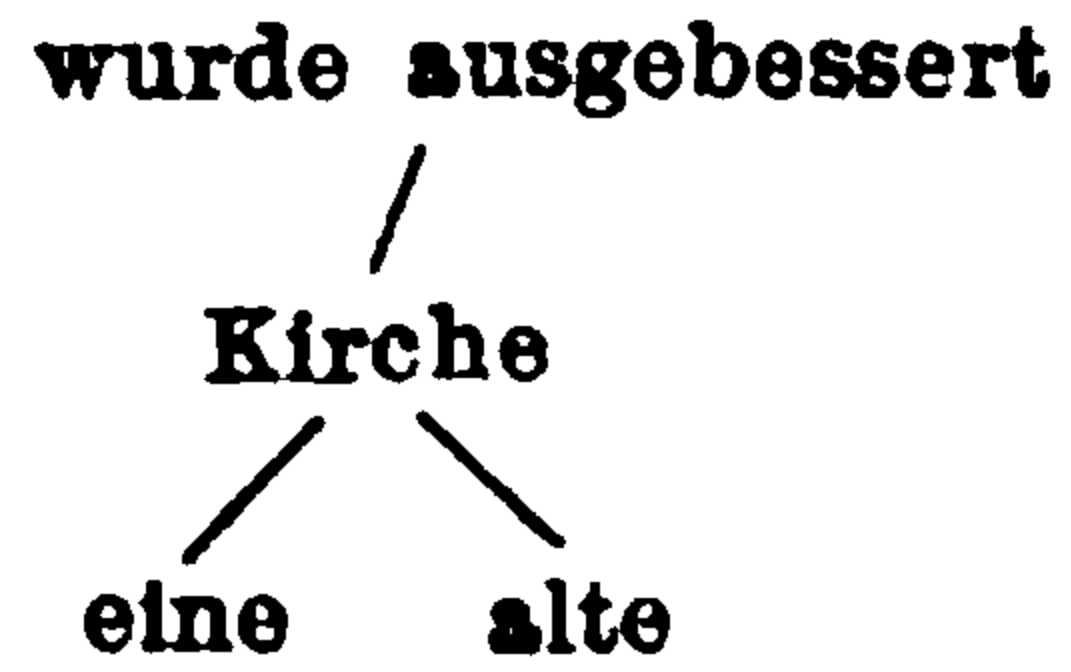
\includegraphics[height=2cm]{figures/Kern1883-1.png}
    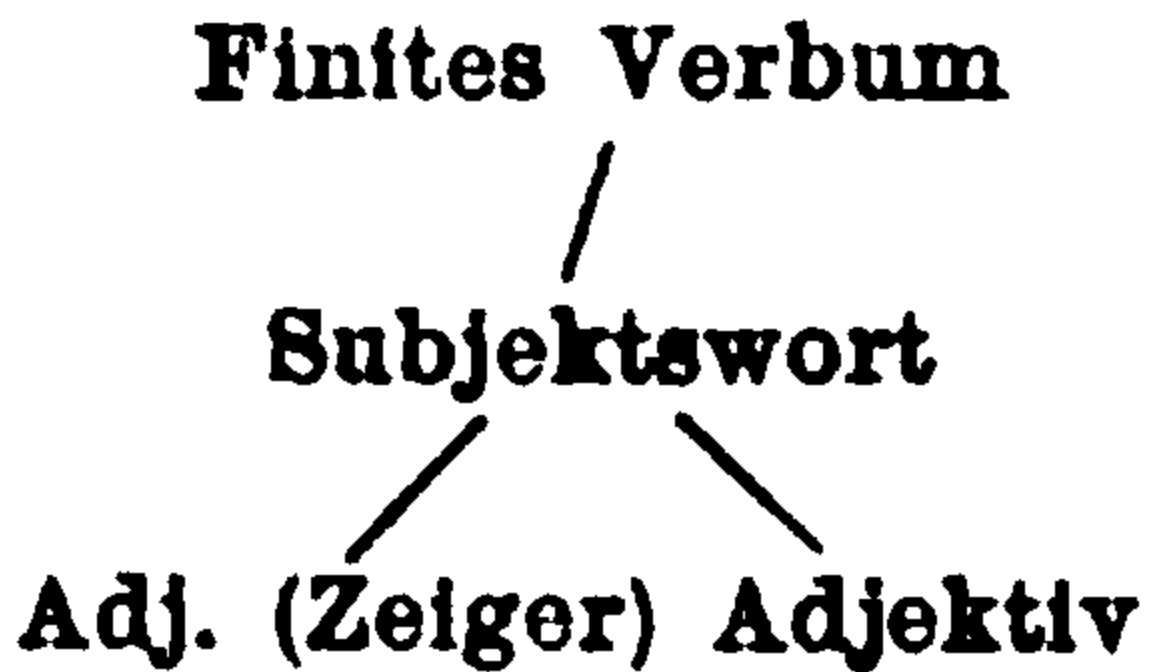
\includegraphics[height=2cm]{figures/Kern1883-2.png}\smallskip\\    
    \noindent\parbox{6cm}{\small\textit{Eine alte Kirche wurde ausgebessert.}\\
    ‘Une ancienne église a été reconstruite.’}
    \end{figure}

    La notion de \textit{valence} a été introduite par le sémioticien anglais Charles S. Peirce dans un article de \citeyear{peirce1897logic}. Peirce compare la possibilité qu’a le verbe \textit{give} ‘donner’ de se combiner avec trois éléments (\textit{John gives John to John}) avec la possibilité qu’à l’atome d’azote N de se combiner avec trois atomes d’hydrogène H pour donner une molécule d’ammoniac NH\textsubscript{3}. Cette métaphore de la connexion entre mots par la connexion entre atomes est accompagnée de la figure suivante :

    \begin{figure}[H]
    \caption{Schéma valenciel de \citet{Peirce1897}}
    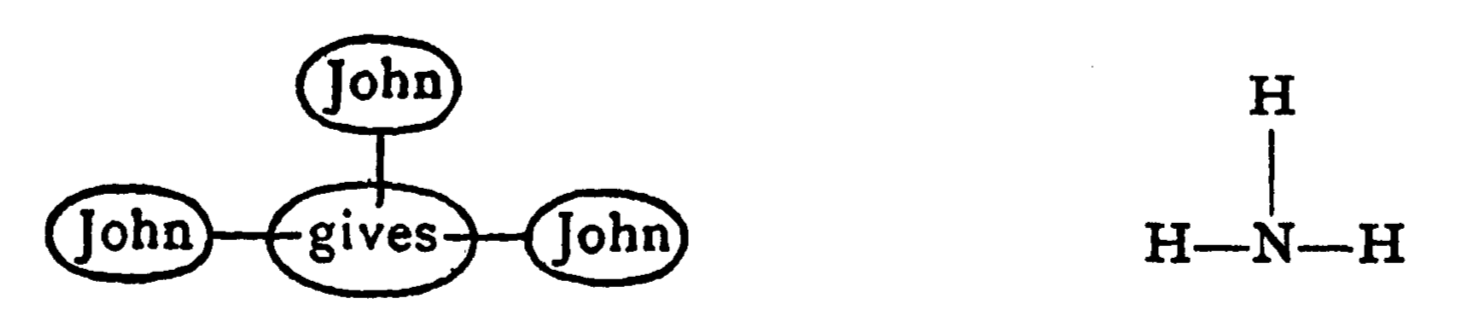
\includegraphics[width=\textwidth]{figures/vol1syntaxe2-img016.png}
    \end{figure}

    Peirce remarque que contrairement aux connections chimiques les connections entre mots (il s’agit plutôt de connexions sémantiques que syntaxiques) sont asymétriques, ce que semble confirmer son diagramme, où les connexions partent du mot \textit{gives} mais s’arrêtent à la bulle de \textit{John}. (Voir la \sectref{sec:3.3.10} sur \textit{Distribution et valence} pour la suite de la discussion.)

    C’est à Lucien Tesnière qu’on attribue les bases théoriques de la syntaxe de dépendance, exposées brièvement dans son article de \citeyear{tesniere1934comment}, \textit{Comment construire une syntaxe}, puis en détail dans son ouvrage posthume de \citeyear{tesniere1959elements}, \textit{Éléments de syntaxe structurale}. On notera, dans l’analyse suivante de 1934, que Tesnière considère la préposition comme dépendant du nom qu’elle introduit. (Le diagramme contient par ailleurs une erreur, qui n’est pas dans le manuscrit de Tesnière : le lien entre \textit{apporte} et \textit{vigueur} a été erronément attribué à \textit{elle}.)

    \begin{figure}[H]
    \caption{Diagramme (tronqué) de \citet{tesniere1934comment}}
    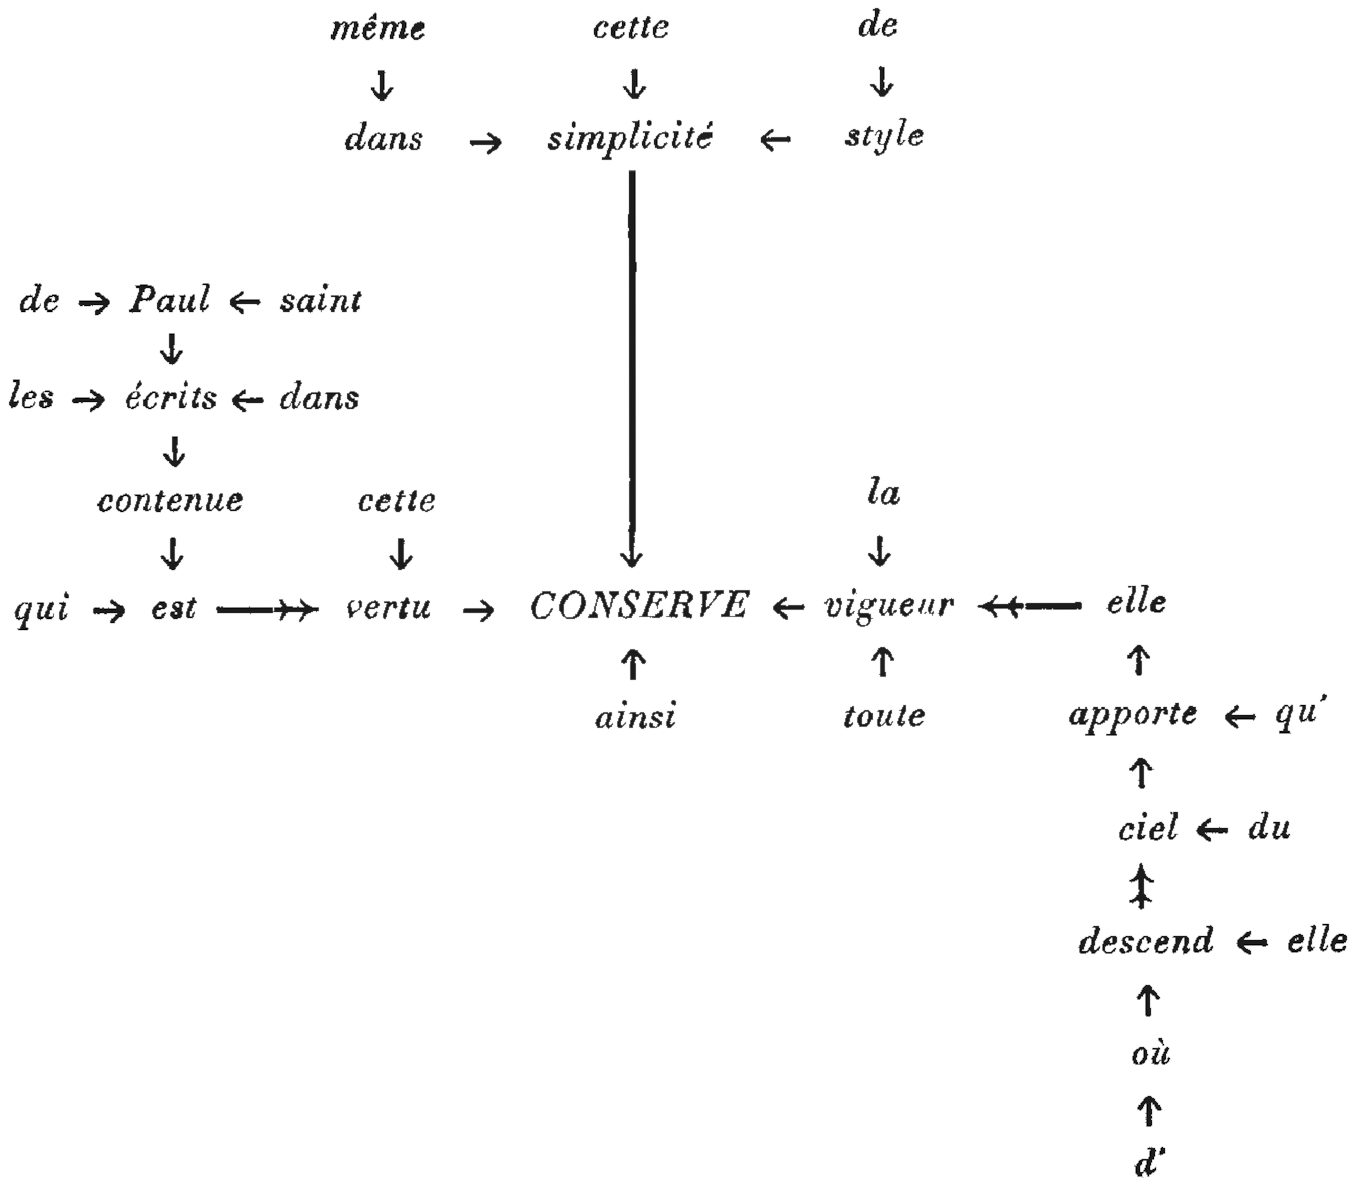
\includegraphics[width=\textwidth]{figures/Tesniere1934.png}\smallskip\\    
    \noindent\parbox{\textwidth}{\small\textit{Ainsi cette vertu céleste, qui est contenue dans les écrits de saint Paul, même dans cette simplicité de style, conserve toute la vigueur qu’elle apporte du ciel d’où elle descend.} (Bossuet)}
    \end{figure}

    Si cette analyse contient déjà des symboles spéciaux (comme les flèches à double pointe \textrm{$\twoheadrightarrow $} pour les relatives), ce n’est que plus tard que Tesnière introduira les symboles en T pour la translation. Les structures de l’ouvrage de 1959 ne sont plus totalement hiérarchique comme le montre notre interprétation polygraphique ci-dessous de la représentation proposée par Tesnière pour \textit{Écrivez dans le livre de votre ami} !.

    \begin{figure}[H]
    \caption{Interprétation polygraphique d'un stemma}
    \begin{subfigure}[b]{.5\textwidth}\centering
% %     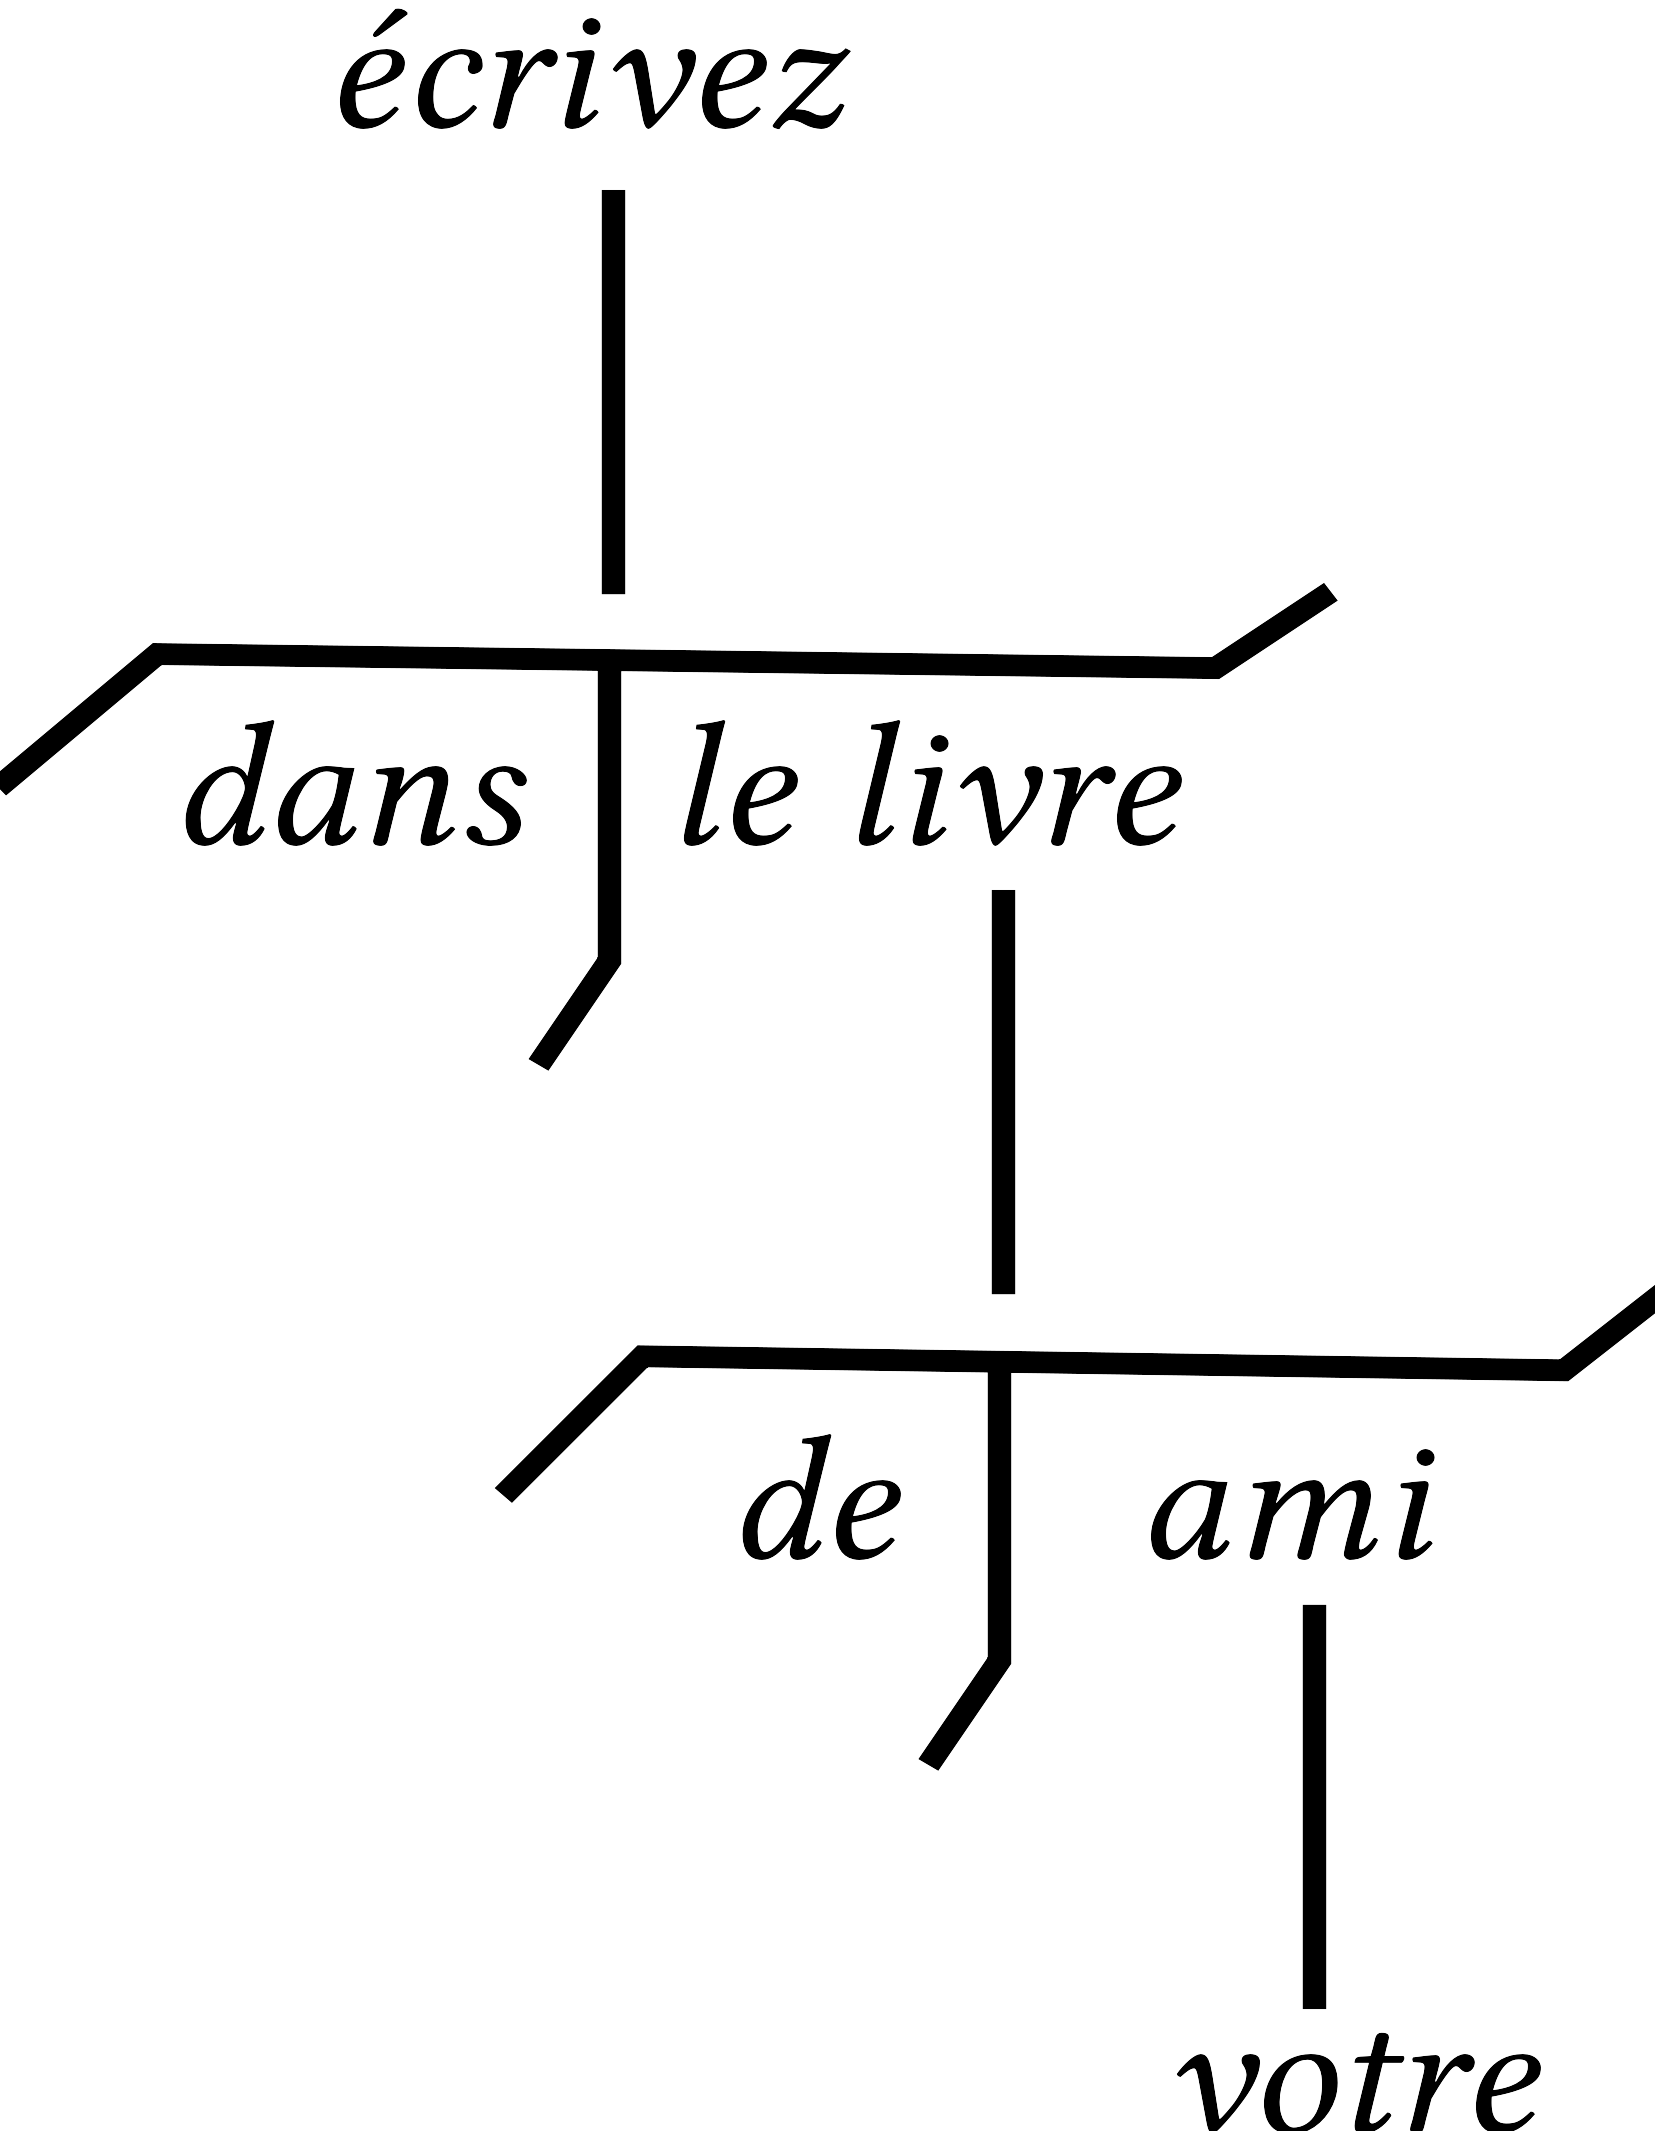
\includegraphics[width=4cm]{figures/StemmadeTesniere}
         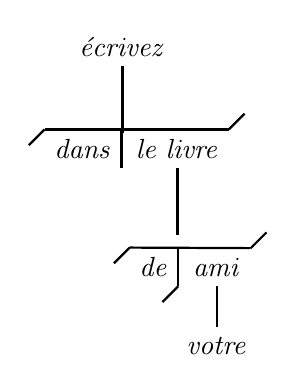
\begin{tikzpicture}
           \node (dans) at (.5,3) {\textit{dans}};
           \node (écrivez) at (1,4.3) {\textit{écrivez}};
           \node (de) at (1.4,1.5) {\textit{de}};
           \node (le livre) at (1.7,3) {\textit{le livre}};
           \node (ami) at (2.2,1.5) {\textit{ami}};
           \node (votre) at (2.2,0.5) {\textit{votre}};
         
           \draw[thick] (dans.north west) -- (le livre.north east);
           \draw[thick] (de.north west) -- (ami.north east);
           \draw[thick] (dans.north east) -- (dans.south east);
           \draw[thick] (de.north east) -- (de.south east);
         
           \draw[thick] (dans.north west) -- +(-2mm, -2mm);
           \draw[thick] (le livre.north east) -- +(2mm, 2mm);
           \draw[thick] (de.north west) -- +(-2mm, -2mm);
           \draw[thick] (ami.north east) -- +(2mm, 2mm);
         
         
           \draw[thick] (de.south east) -- +(-2mm, -2mm);
         
           \draw[thick,shorten >=2mm] (écrivez) -- (1,3);
           \draw[thick,shorten >=4mm] (le livre) -- (1.7,1.5);
           \draw[thick] (ami) -- (votre);
         \end{tikzpicture}
    \caption{Stemma de \citet{tesniere1959elements}}
    \end{subfigure}%
    \begin{subfigure}[b]{.5\textwidth}\centering
% %     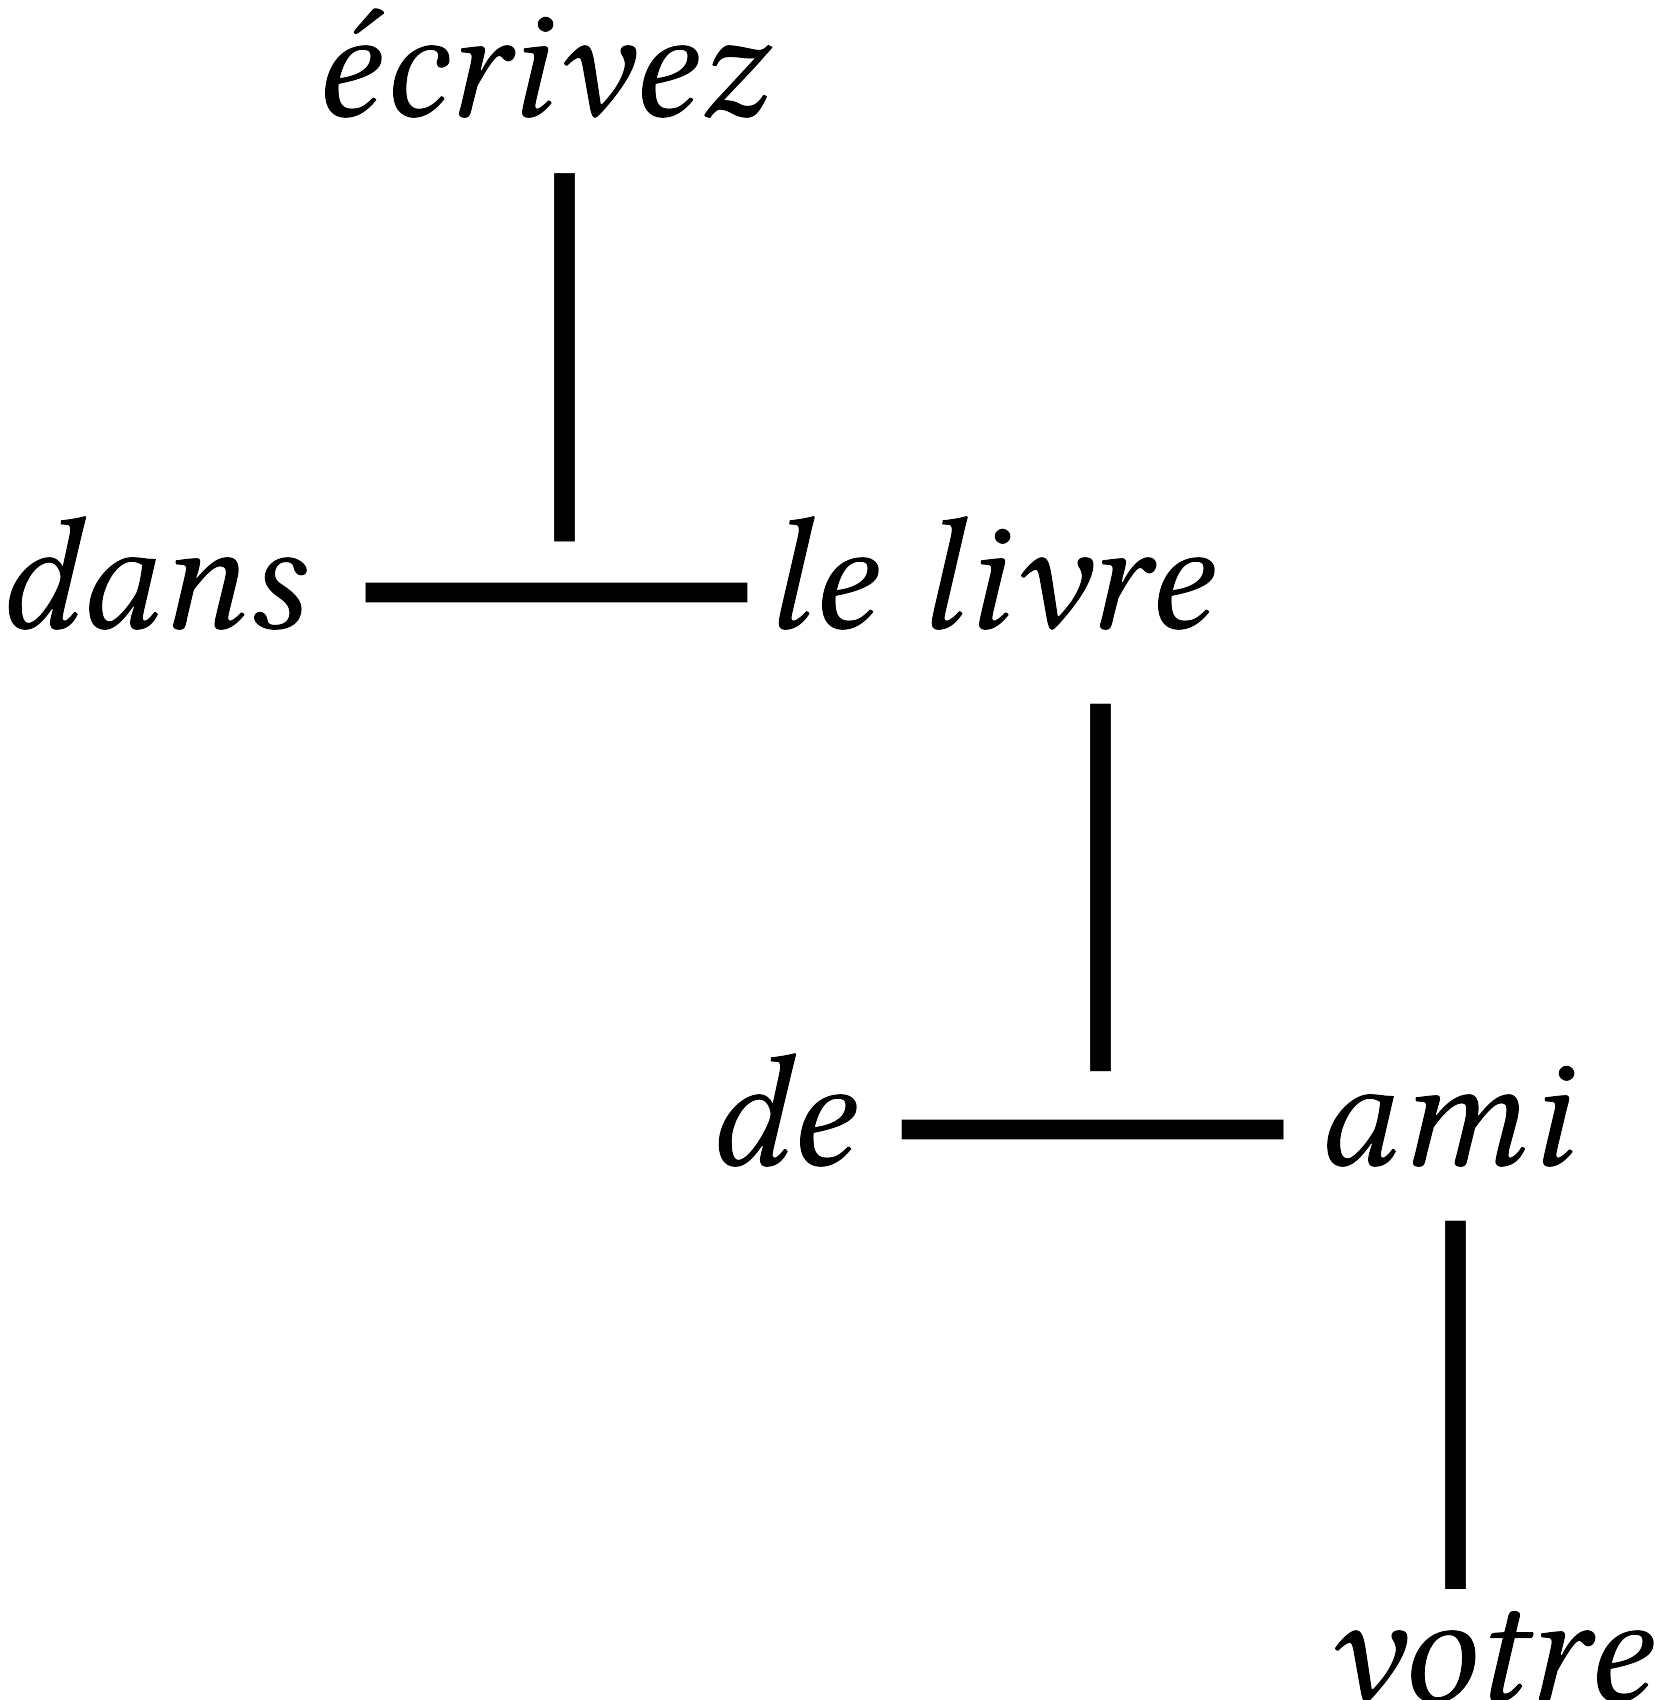
\includegraphics[width=4cm]{figures/Stemma}
        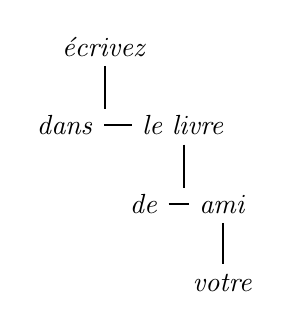
\begin{tikzpicture}
          \node (dans) at (.5,3) {\textit{dans}};
          \node (écrivez) at (1,4) {\textit{écrivez}};
          \node (de) at (1.5,2) {\textit{de}};
          \node (le livre) at (2,3) {\textit{le livre}};
          \node (ami) at (2.5,2) {\textit{ami}};
          \node (votre) at (2.5,1) {\textit{votre}};
        
          \draw[thick] (dans) -- (le livre);
          \draw[thick] (de) -- (ami);
          \draw[thick,shorten >=2mm] (écrivez) -- (1,3);
          \draw[thick,shorten >=2mm] (le livre) -- (2,2);
          \draw[thick] (ami) -- (votre);
        \end{tikzpicture}
    \caption{Interprétation polygraphique}
    \end{subfigure}
    \end{figure}
\todo[inline]{figure (a): the T shape of "de ami" is ok. The T shape of "dans le livre" must be identical, including the small space on top.}
\todo[inline]{figure (b): the line between "dans" and "le livre" must be longer and the vertical line must be centered on the horizontal line. Idem for "de" and "ami". .}
}

\section{Arbre et représentation planaire}\label{sec:3.3.6}

Il est essentiel de rappeler que la \hi{représentation par un arbre} (\hi{de dépendance)} sert uniquement à encoder une \hi{structure hiérarchique} liant des nœuds entre eux par des relations père-fils. Dès qu’un arbre est représenté sur une feuille plane, les nœuds frères (c’est-à-dire ayant le même père) doivent être placés les uns à côté des autres et apparaissent donc comme ordonnés. Cet ordre sur les nœuds frères, imposé par la \hi{représentation planaire}, est souvent utilisé pour encoder d'autres informations comme la saillance syntaxique (chez Tesnière par exemple) (voir \chapfuturef{15}) ou la saillance communicative (chez les Pragois) (voir l'\encadref{3.5.24} \textit{Ordre communicativement dirigé}). Un arbre avec un ordre sur les nœuds frères est une structure plus riche qu’un simple arbre. Les arbres que nous considérons dans ce chapitre sont des \hi{arbres non ordonnés}. Il faut se les imaginer dans l’espace, libérés de la feuille, comme des \hi{mobiles} suspendus dans l’air et dont les nœuds peuvent tourner librement autour de leur gouverneur.

Pour en faciliter la lecture, nous placerons généralement les nœuds de nos arbres dans l’ordre qu’ils occupent dans la phrase, mais cet ordre n’a aucune pertinence lorsque l’arbre est considéré en tant que tel et nos lecteurs devront essayer d’en faire abstraction. Libérez les arbres de la feuille ! Faites-les tourner dans votre tête !

Nous allons maintenant voir comment définir l’arbre de dépendance. Pour cela nous allons introduire différents critères permettant d’identifier la tête d’une unité syntaxique.

\section{Critère d’effacement simple et critère prosodique}\label{sec:3.3.7}

Une première définition possible d’une structure de dépendance se base sur la structure de connexion. Lorsqu’on possède déjà une structure de connexion, on peut la hiérarchiser (au moins partiellement) simplement en choisissant un nœud racine dans la structure. On peut alors orienter les connexions en partant de la racine. Tout se passe comme si on attrapait la structure par ce nœud et qu’on la suspendait.

Illustrons cela avec la phrase :

\ea \textit{Pierre veut inviter Marie demain.}\z

Si l’on a la structure de connexion de cette phrase (voir \chapref{sec:3.2}) et qu’on peut établir que \textit{veut} est la tête (voir \sectref{sec:3.3.8} suivante), on obtient immédiatement une structure de dépendance par le procédé que nous venons de décrire, comme le montre la figure \ref{fig:hierarchie}. La flèche blanche
\todo[inline]{The text must be finalized when the types of the arrows have been decided.}
indique le nœud par lequel on attrape la structure pour la hiérarchiser. Ce nœud va gouverner les nœuds auxquels il est connecté, lesquels vont gouverner à leur tour les nœuds auxquels ils sont connectés et ainsi de suite.

\begin{figure}
\vskip\baselineskip
\caption{Hiérarchisation d'une structure de connexion\label{fig:hierarchie}}
\begin{tabular}{@{}>{\centering}m{5cm} m{2em} >{\centering\arraybackslash}m{5cm} @{}}
  \begin{tikzpicture}
    \begin{scope}[every node/.style={ConcSet}]
    \node at (0,0)   (Pierre) {Pierre};
    \node at (1,-1.5)  (veut) {veut};
    \node at (2,0)   (inviter) {inviter};
    \node at (3,1.5)   (Marie) {Marie};
    \node at (3,-1.5)  (demain) {demain};
    \draw (Pierre) -- (veut) -- (inviter) -- (Marie);
    \draw (inviter) -- (demain);
    \end{scope}
    \node [below left=1mm of veut, single arrow, draw, inner sep=1pt, 
           minimum height=1.5em, shape border uses incircle, shape border rotate=45] {};
  \end{tikzpicture} 
  & {\huge$\Rightarrow$} 
  & \begin{tikzpicture}
  \begin{scope}[every node/.style={ConcSet},
                        edge from parent/.style={draw,-{Triangle[]}},
                        sibling distance=2cm
                        ]
  \node (root) {veut}
    child { node {Pierre} }
    child { node {inviter} 
            child { node {Marie} }
            child { node {demain } }
    };
  \end{scope}
  \node [above=1mm of root, single arrow, draw, inner sep=1pt, minimum height=1.5em,
           shape border uses incircle, shape border rotate=270] {};
  \end{tikzpicture}\\
  Structure de connexion & & Arbre de dépendance
\end{tabular}
\end{figure}

Si la structure de connexion n’a que des connexions élémentaires (voir l’\encadref{sec:3.2.23} \textit{Graphe à bulles et polygraphe}) et pas de cycles, on obtient un arbre de dépendance, comme dans l’exemple précédent.

Baser ainsi la dépendance sur la connexion, revient à donner une importance première aux propriétés définitoires des unités syntaxiques, l’\textstyleTermes{autonomisabilité illocutoire} et l’\textstyleTermes{autonomisabilité prosodique} (voir la \sectref{sec:3.2.11} \textit{Unité syntaxique autonomisable}). Traduit pour le repérage de la tête d’une unité, ces deux critères deviennent le critère d’effacement simple et le critère prosodique.

L’autonomisabilité illocutoire donne le critère suivant.

\Definition{Critère d’effacement simple}
{\textstyleTermes{Critère d’effacement simple} : si \hi{l’unité} AB \hi{est gouvernée par} X et que B \hi{peut être effacé}, mais pas A, alors A \textbf{est la tête de} AB et B dépend de A.}

Dire que B peut être effacé et pas A lorsque AB est gouverné par X revient à dire que XA peut former une unité (illocutoirement) autonome, mais pas XB et donc que X est connecté à A. Comme X est le gouverneur de AB, on en déduit que A est la tête de AB.

On peut illustrer l'application du critère d'effacement simple sur le syntagme \textit{demain matin} dans la phrase \textit{Pierre part demain matin.}
On a donc X = \textit{part,} A = \textit{demain} et B = \textit{matin}. Une fois établi que X est la tête de la phrase et gouverne donc AB, alors on en déduit que B dépend de A, car B est effaçable (\textit{Pierre part demain}), mais pas A (*\textit{Pierre part matin}).

\begin{figure}
\begin{tikzpicture}[baseline]
\node at (0,0) (X) {X};
\node at (1.5,0) (A) {A};
\node at (2.5,0) (B) {B};

\node [draw,ellipse,inner sep=0pt,fit=(A) (B)] (AB) {};
\draw (A) -- (B);
\draw [-{Triangle[]}] (X) -- (AB);

\node at (4,0) {\huge$\Rightarrow$};
\node at (5,0) (X2) {X};
\node at (6,0) (A2) {A};
\node at (7,0) (B2) {B};

\draw [-{Triangle[]}] (X2) -- (A2);
\draw [-{Triangle[]}] (A2) -- (B2);
\end{tikzpicture}
\caption{\label{fig:}Application du critère d’effacement simple}
\end{figure}

Attention : la présence d’un gouverneur est essentielle dans la formulation du  critère d’effacement simple. On trouve souvent la \textbf{mauvaise formulation} suivante : le dépendant d’une connexion est l’élément qui peut le plus facilement être effacé. Cette propriété n’est valable qu’en présence d’un gouverneur. Si AB est un énoncé autonome ou plus généralement si AB n’est pas gouverné on peut très bien effacer la tête de AB. Par exemple, dans \textit{Zoé chantait} (A = \textit{chantait}, B = \textit{Zoé}), on peut effacer A et pas B (\textit{Zoé} peut former un énoncé autonome, mais pas \textit{chantait}), alors que c’est A qui est la tête !

Passons maintenant à l’autonomisabilité prosodique, le deuxième critère qui nous a permis de définir la structure de connexion. L’autonomisabilité prosodique donne le critère suivant.

\Definition{\textstyleTermes{critère prosodique}}
{\textstyleTermes{critère prosodique~}: si X est le gouverneur de AB et si X \textbf{peut former une unité prosodique avec} A sans B (sans changer significativement le sens), alors A est \textbf{la tête de l’unité} AB.}

Le critère prosodique reste d'un utilisation marginale et nous n'en donnerons pas d'exemple d'application.

Les deux critères que nous venons de proposer sont insuffisants pour plusieurs raisons.

Premièrement, ils ne s’appliquent que dans le cas où l’on étudie une unité qui possède un gouverneur. Ils ne peuvent donc pas être utilisés pour déterminer la tête d’un énoncé. Ce point va être étudié dans la section suivante.

Deuxièmement, il est assez courant que deux éléments qui se combinent soient indissociables, à l’intérieur du mot bien sûr (\textit{chant-ons}), mais aussi en dehors, comme \textit{le} et \textit{chien} dans \textit{le chien dort}. Dans ce cas, le critère d’effacement simple ne s’applique pas, pas plus que le critère prosodique en général.

Troisièmement, le critère d’effacement simple est inopérant si B est un dépendant obligatoire de A. C’est le cas pour une combinaison comme \textit{à Marie}, où A = \textit{à} ne peut pas s’employer sans son complément B et ne peut donc jamais former une unité XA avec le gouverneur X de AB. C’est encore le cas pour les formes verbales finies de langues comme le français : en effet, pour \textit{Marie dormait}, il n’est pas possible de vérifier si A = \textit{dormait} peut former une unité avec un éventuel gouverneur X, puisque A ne s’emploie jamais sans un sujet B. Ceci a d’ailleurs amené Leonard Bloomfield (qui fut le premier, dans son ouvrage \textit{Langage} de \citeyear{bloomfield1933language}, à proposer des critères pour définir la tête) à considérer que ces constructions sont \textstyleTermes{exocentriques,} c’est-à-dire sans tête (voir la \encadref{sec:3.3.2} \textit{Historique des notions de dépendance et de tête}.)

Les limites du critère d’effacement simple et du critère prosodique nous amènent à introduire d’autres critères plus puissants. Dans les critères que nous venons de considérer, le gouverneur X de l’unité AB que l’on étudie est fixé. On regarde seulement ce qui se passe dans une phrase donnée, sans faire varier X, A ou B. Cela confère à ces critères une grande simplicité d’utilisation, mais c’est aussi une limite. L’analyse distributionnelle va nous permettre de donner une version plus riche et plus fiable du critère d’effacement : le \textstyleTermes{critère distributionnel avec effacement}, présenté dans la \sectref{sec:3.3.11} éponyme.

\section{Tête d’un énoncé}\label{sec:3.3.8}

Comme nous l’avons vu à la section précédente, nous avons des critères pour identifier la tête d’une unité dès qu’on connaît son gouverneur, mais ces critères ne peuvent pas s’appliquer pour caractériser la tête d’un énoncé. Or, tant qu’on n’a pas identifié celle-ci et qu’on n’a pas un premier gouverneur, on ne peut pas appliquer le critère d’effacement simple ou le critère prosodique.

L’identification de la tête d’un énoncé repose sur les propriétés de l’énoncé en tant que tel, à savoir le fait qu’il fait l’objet d’une énonciation dirigée vers un interlocuteur et qu’il possède donc une \textstyleTermes{fonction illocutoire}. Cette notion repose sur le constat que produire un énoncé est une véritable action de la part du locuteur (on parle d’\textstyleTermes{actes de langage}, à la suite des travaux de \citet{gardiner1932speech}, John \citet{austin1962how} et John \citet{searle1969speech}), qui attend généralement en retour une action du ou des destinataire(s) (voir également la contribution de \citet{bloomfield1933language} dans la \sectref{sec:1.1.4} \textit{Sens et intention communicative}).

Ceci nous amène à considérer quatre types d’énoncés : \textstyleTermes{assertion}, \textstyleTermes{question}, \textstyleTermes{injonction} et \textstyleTermes{exclamation}.

\begin{itemize}
\item assertion : \textit{«~Il pleut.~»~}; \textit{«~J’ai mal au ventre.~»~};
\item question : «~\textit{Comment faire ?~»~}; «~\textit{Est-ce un problème ?~»} ;
\item injonction : «~\textit{Laissez ça ici !~»} ;
\item exclamation : «~\textit{Aie !~»~}; «~\textit{Comme c’est sympa !~».}
\end{itemize}

Les assertions peuvent être acceptés ou refusées par le destinataire ; elles se caractérisent par le fait de pouvoir être falsifiées par «~\textit{C’est faux.}~» ou au contraire validées par «~\textit{C’est vrai.}~». Par exemple, si quelqu’un nous dit «~\textit{J’ai mal au ventre}.~», on peut lui répondre «~\textit{C’est faux.}~», mais s’il dit «~\textit{Aie} !~», ce n’est plus possible. De même, on ne peut répondre «~\textit{C’est faux.}~» a une question ou une injonction. Les questions attentent une réponse. Les injonctions attendent généralement un acte non verbal. Les exclamations attendent simplement d’être partagées par le destinataire éventuel.

La fonction illocutoire a souvent un marquage spécifique. Les éléments qui servent à marquer la fonction illocutoire seront appelés des \textstyleTermes{marqueurs illocutoires}. La fonction illocutoire de l'énoncé conditionne son contexte, caractérise le type d'action que va effectuer en retour l'interlocuteur : acquiescer, répondre, obéir, etc. En conséquence, on considère que l'élément de l'énoncé qui porte la fonction illocutoire est la tête de l'énoncé.

\Definition{\textstyleTermes{critère illocutoire}}
{\textstyleTermes{critère illocutoire}. Les \textbf{marqueurs illocutoires} sont \textbf{portés} par la \textbf{tête syntaxique de l’énoncé} et la caractérise.}

En français, le principal marqueur illocutoire est la prosodie (transcrit à l’écrit par des signes de ponctuation comme « ?~» ou « !~»). Mais pour les énoncés à tête verbale en français, il existe d’autres marques. Voyons sur un exemple :

\ea
\textit{{Pierre a dormi}.}
\z

Cet énoncé est une assertion. Comme toute assertion, on peut la nier en répondant «~\textit{C’est faux}~».~La négation de cet énoncé (c'est-à-dire un énoncé ayant pour sens ‘il est faux que Pierre a dormi’) peut s’exprimer en français par un double marquage \textit{ne…pas} qui semble bien identifier l’auxiliaire comme la tête :

\ea
\textit{{Pierre} \textbf{{n’a}  {pas}}  {dormi.}}
\z

On peut également faire varier la fonction illocutoire et transformer cet énoncé en une question ou une injonction :

\ea
  \ea \textit{Pierre \textbf{a-t-il} dormi ?}
  \ex \textit{\textbf{Ais}  dormi (quand  je reviens)!}
  \z
\z

Le français a pour cela des formes particulières : une question peut prendre la \textstyleTermes{forme} dite \textstyleTermes{interrogative}, qui se caractérise par la présence d’un \textstyleTermes{enclitique} (\textit{{}-t-il} dans notre exemple) ; une injonction peut s’exprimer par une forme verbale particulière : l’\textstyleTermes{impératif} (ici \textit{ais}, forme impérative du verbe \textsc{avoir}). C’est encore une fois l’auxiliaire qui est touché, ce qui confirme son statut de tête.

On peut par la même méthode identifier la tête d’une phrase complexe avec deux verbes finis. Cette tête est traditionnellement appelée le \textstyleTermes{verbe principal}. Considérons :
\ea
\textit{{Marie pense que Pierre dort}.}
\z
La forme interrogative est \textit{Marie pense-t-elle que Pierre dort} ? et pas *\textit{Marie pense que Pierre dort-il} ? On en déduit que \textit{pense} est la forme verbale principale et que \textit{dort} est une forme verbale subordonnée.

\Definition{\textstyleTermes{subordination}, \textstyleTermes{proposition subordonnée}}
{La \textstyleTermes{subordination} est simplement le terme traditionnel pour désigner la \hi{dépendance d’une forme verbale} à un autre élément.  Une proposition dont le verbe est subordonné est appelée une \textstyleTermes{proposition subordonnée}.}

On appelle \textstyleTermes{proposition} une unité de taille maximale dont la \hi{tête} est une \hi{forme verbale}. Nous donnerons une définition plus précise de la proposition dans la \sectref{3.3.30} sur \textit{Dominance et projections maximales}.

L’identification de la subordination nous procure un nouveau test pour repérer la tête d’une proposition (voir \hi{critère rectionnel} à la \sectref{sec:3.3.16} \textit{Tête interne et critère rectionnel}). En effet, certains verbes imposent un mode particulier à leur subordonné. Par exemple, si l’on subordonne au verbe \textsc{falloir} la proposition \textit{Pierre a dormi}, on obtient \textit{Il faut que Pierre} \textbf{\textit{ait}} \textit{dormi (quand je reviens).} Comme on le voit, encore une fois, c’est l’auxiliaire qui hérite ici de la marque de subordination, à savoir le \textstyleTermes{mode subjonctif} (\textit{ait} est une forme subjonctive de \textsc{avoir}), ce qui confirme son statut de tête syntaxique de la proposition.

On peut encore utiliser ces différents critères pour repérer que certains énoncés n’ont pas une tête verbale. Comparons les deux phrases suivantes :

\ea 
  \ea \textit{Heureusement, Pierre a dormi.}
  \ex \textit{Heureusement que Pierre a dormi.}
  \z
\z

On peut subordonner le premier énoncé, mais pas le deuxième :

\ea
  \ea[]{\textit{Je crois que, heureusement, Pierre a dormi.}}
  \ex[*]{\textit{Je crois qu’heureusement que Pierre a dormi.}}
  \z
\z

Comme il apparaît par ailleurs que le verbe \textsc{croire} peut subordonner n’importe quelle proposition à l’indicatif, on peut supposer que la phrase introduite par \textit{heureusement que} ne peut pas être subordonnée car le verbe n’en est pas la tête. On en déduit que \textit{heureusement} est la tête de la phrase et subordonne la proposition \textit{Pierre a dormi} (ce que confirme l’emploi de la conjonction de subordination \textit{que}).

Le même type de raisonnement permet d’identifier la tête d’une proposition dans n’importe quelle langue a priori (voir encadré ci-dessous).

\globe[sec:3.3.9]{Tête d’un énoncé dans une langue inconnue}{%
    Comme nous l’avons dit dans les sections précédentes, l’identification de la tête d’un énoncé est un préalable à la hiérarchisation de la structure.

    Nous allons considérer le cas de deux langues non apparentées, l'anglais et le coréen. Le cas du wolof sera présenté dans la \sectref{3.3.16} sur \textit{Tête interne et critère rectionnel}.
    
  Commençons par l’\hi{anglais}, qui est une langue très proche du français, mais dont le fonctionnement est quand même assez différent. Considérons l’énoncé \textit{Peter has slept} ‘Pierre a (déjà) dormi’. Comme en français, la négation va sur l’auxiliaire sur lequel elle se cliticise :
    \ea
        \textit{{Peter} \textbf{{hasn’t}}  {slept.}} \\\glt ‘Pierre n’a pas dormi.’
    \z
    Quant à la question, elle est normalement formée par l’antéposition de l’auxiliaire :
    \ea
        \textit{\textbf{{Has}}  {Peter slept?}} \\\glt   ‘Pierre a-t-il dormi ?’
    \z
    On peut considérer que cette place particulière de l’auxiliaire le marque comme la tête. D’ailleurs, un verbe ordinaire ne peut recevoir directement la négation, ni être antéposé. Le passage à une forme interrogative ou négative nécessite l’introduction de l’auxiliaire \textsc{do} ‘faire’ :
    
    \ea
      \ea \textit{Peter slept.}  \\\glt  ‘Pierre a dormi.’
      \ex \textit{\textbf{{Did}}  {Peter sleep?}}  \\\glt  ‘Pierre a-t-il dormi ?’
      \ex \textit{{Peter} \textbf{{didn’t}}  {sleep.}} \\\glt ‘Pierre n’a pas dormi.’
      \z
    \z
    Comme on le voit, la forme passé \textit{slept} passe à la forme infinitive. L’auxiliaire lui-même hérite de la finitude (\textit{did} est la forme passé de \textsc{do}) et constitue donc la tête de la phrase quand il est présent. En l’absence d’auxiliaire, c’est la forme verbale simple qui est la tête, puisque c’est elle qui est affectée lorsque l’auxiliaire est introduit. On notera que l’auxiliaire, bien qu’il soit la tête de la phrase, peut dans certains cas se cliticiser sur le sujet (c’est-à-dire perdre la possibilité de recevoir un accent tonique et former un mot prosodique avec le dernier mot du sujet) :
    
    \ea
      \ea \textit{{Peter}\textbf{{’s}}  {sleeping}} =  \textit{{Peter} \textbf{{is}}  {sleeping}} \\\glt ‘Pierre est en train de dormir’, lit. Pierre est dormant.
      \ex \textit{{Peter}\textbf{{’s}}  {eaten}}   =   \textit{{Peter} \textbf{{has}}  {eaten}}  \\\glt ‘Pierre a (déjà) mangé’
        \z
    \z
   
   En \hi{coréen}, le verbe principal d’un énoncé est caractérisé par un marqueur de politesse qu’il est le seul à pouvoir porter. Cette particule s’ajoute optionnellement sur le verbe principal, mais jamais sur un verbe subordonné. Le coréen utilise essentiellement des constructions à verbe support (voir \encadref{2.3.9} sur \textit{Verbes supports et unités grammaticale}s) avec le verbe \textsc{hada} ‘faire’. Dans la phrase suivante, le sens ‘aimer’ est ainsi lexicalisé par le nom \textsc{sarang} ‘amour’ et le sens ‘croire’ par le nom \textsc{saenggak} ‘pensée’, tous deux «~verbalisés~» par le verbe \textsc{hada}. La deuxième occurrence de \textsc{hada} peut porter le morphème de politesse \textit{yo}, mais pas la première. (Nous reviendrons sur les marqueurs illocutoires du coréen dans l’encadré \textit{Des prédicatifs uniquement locutifs assertifs} du \chapfuturef{17}.)

    \ea \let\eachwordone\cjkfont
    \ea[]{
    \gll  철수가 나를 사랑한다고 생각해(-\textbf{요})\\
    \textit{Ch’ŏlsu-ga} \textit{na-rŭl} \textit{sarang-ha-ndago} s\textit{aenggak-hae}(-\textit{\textbf{yo}})\\
    Ch’ŏlsu-\textsc{nom}   moi-\textsc{acc}  amour-faire-\textsc{pres.inf}  pensée-faire(-\textsc{politesse)}\\
    \glt   ‘Je crois que Cholsu m’aime’}
    \ex[*]{
    \gll   철수가 나를 사랑해-\textbf{요}다고 생각해(-\textbf{요})\\
    \textit{Ch’ŏlsu-ga}            \textit{na-rŭl}            \textit{sarang-hae-\textbf{yo}-dago}  \textit{saenggak-hae}(-\textit{\textbf{yo}})\\
    Ch’ŏlsu-\textsc{nom}  moi-\textsc{acc}  amour-faire-\textsc{politesse}-\textsc{pres.inf}  pensée-faire(-\textsc{politesse)}\\}
    \z
    \z
}
\section{Distribution et valence}\label{sec:3.3.10}

En nous basant sur la structure de connexion et en déterminant la tête de la proposition grâce aux marqueurs illocutoires, nous avons vu que nous pouvions obtenir une structure de dépendance partielle. Nous allons voir que l’on peut raffiner cette structure en ajoutant des critères additionnels. Les premiers de ces critères sont les critères distributionnels que nous présenterons dans les sections suivantes. Nous devons avant cela introduire les notions de distribution (voir l'\encadref{sec:2.1.7} sur \textit{L’identification des unités de la langue}, où il a été question d’analyse distributionnelle) et valence (voir la \sectref{sec:3.3.5} \textit{Historique des représentations syntaxiques par des diagrammes en dépendance} pour un début de discussion).

\Definition{\textstyleTermes{distribution}}
{La \textstyleTermes{distribution} d’une unité est l’\hi{ensemble des contextes} ou \hi{environnements} où peut se trouver cette unité.}

Deux remarques essentielles sont à faire concernant la distribution.

Premièrement, nous faisons de l’analyse distributionnelle sur un objet structuré. Ici, ce qui nous intéresse, c’est la \textstyleTermes{distribution syntaxique} et non la distribution linéaire. Nous nous intéressons donc au contexte des unités au sein de la structure syntaxique, c’est-à-dire au \textstyleTermes{paradigme} des unités qui se combinent avec l’unité que nous étudions.

La notion de distribution est encore exprimable en termes de valence.

\Definition{\textstyleTermes{valence}}
{La \textstyleTermes{valence} d’une unité syntaxique est la \hi{capacité} qu’à cette unité \hi{à se combiner} avec d’autres unités syntaxiques. La valence est avant tout une \hi{valence potentielle}, à contraster avec la \hi{valence réalisée}, lorsque l’unité est utilisée dans un contexte donné.}

Cette métaphore de la valence est inspirée de la chimie et de la capacité qu’à un atome à \hi{se combiner avec d’autres atomes pour former des molécules} (voir la contribution de \citet{Peirce1897} dans l’\encadref{sec:3.3.5} \textit{Historique des représentations syntaxiques par des diagrammes en dépendance}, ainsi que les formules utilisées par \citet{jespersen1937analytic}, évoquées dans l’\encadref{sec:3.3.2} \textit{Historique des notions de dépendance et de tête}). Mais alors que les connexions entre atomes sont symétriques (chaque atome fournit un électron de même nature), les connexions entre unités sont doublement asymétriques : \hi{asymétrie syntaxique}, puisqu’elles lient un gouverneur à un dépendant, et \hi{asymétrie sémantique}, puisqu’elle lient un prédicat à un argument.

L’asymétrie syntaxique nous amène à distinguer deux parties dans la valence.

\Definition{\textstyleTermes{valence supérieure}}
{La \textstyleTermes{valence supérieure} d’une unité syntaxique U est la \hi{position syntaxique} occupée par le \hi{gouverneur} de U, cette position étant elle-même caractérisée par le \hi{paradigme} des éléments qui peuvent l’occuper.}

\Definition{\textstyleTermes{valence inférieure}}
{A l’inverse, la \textstyleTermes{valence inférieure} d’une unité syntaxique est l’ensemble des positions syntaxiques qui \hi{dépendent} potentiellement de cette unité.}

Les notions de valences supérieure et inférieure ont été introduites par Igor Mel’čuk, qui les nomment \textit{valence passive} et \textit{valence active}. Nous préférons éviter le terme de \textit{valence passive}, un peu trompeur dans le cas des modifieurs, qui prennent leur gouverneur syntaxique dans leur valence sémantique (voir \chapfuturefici{13}).

Deuxièmement, nous souhaitons utiliser l’analyse distributionnelle pour caractériser la tête d’une unité. Nous cherchons donc à repérer dans le contexte syntaxique d’une unité le contexte qui caractérise plus particulièrement la tête, c’est-à-dire la valence supérieure.

Illustrons ce dernier point par un exemple. Considérons l’énoncé \textit{Une très vieille dame habite ici} et l’unité syntaxique \textit{vieille dame} qu’il contient. Aucun des deux mots \textit{vieille} et \textit{dame} ne contrôlent à lui seul l’entièreté de la distribution de l’unité qu’ils forment ensemble, car \textit{vieille} est connecté à \textit{très} (\textit{très vieille}) et \textit{dame} est connecté à \textit{une} et \textit{habite} (\textit{une dame habite ici}). Bien sûr, une fois que l’on sait que \textit{habite} est la tête de la phrase, on en déduit que la tête de \textit{vielle dame} est \textit{dame}, puisque c’est le mot qui est connecté au gouverneur de cette unité syntaxique.

On ne dira jamais assez qu’on ne peut \hi{déterminer la tête} d’une unité syntaxique U par la distribution qu’\hi{une fois qu’on} \hi{a déterminé la valence supérieure} de U, c’est-à-dire qu’on a déterminé qui parmi les éléments auxquels U est connectée gouverne U. Considérer la distribution sans avoir au préalable distingué valence inférieure et supérieure peut conduire à des erreurs méthodologiques. Il y a là un cercle vicieux dans lequel il faut éviter de rentrer, puisqu’on ne peut appliquer de critère distributionnel pour déterminer la tête d’une unité sans savoir où se trouve son gouverneur. Autrement dit, il s’agit d’un critère pour déterminer la hiérarchie qui ne peut s’appliquer qu'en connaissant déjà une partie de la hiérarchie.

Supposons que l’on veuille déterminer qui du nom ou du déterminant est la tête du groupe qu’ils forment ensemble (comme par exemple \textit{chat} et \textit{le} dans \textit{le chat dort}). Si l’on décrète que pouvoir être sujet d’un verbe fait partie de la valence supérieure du nom, le problème est biaisé, puisque, en un sens, on a déjà décidé que le nom est la tête du groupe qu’il forme avec le déterminant (on trouve cette erreur méthodologique dans l’ouvrage de référence d’Igor Mel’čuk de \citeyear{melcuk1988dependency}). Tout le problème ici est qu’on ne peut facilement déterminer la valence supérieure du nom seul, car, dans de nombreuses positions, il est indissociable d’un déterminant. (Voir la \sectref{sec:3.3.23} sur \textit{Nom ou déterminant comme tête} ?) Nous avons contourné ce problème en définissant au préalable la structure de connexion (\chapref{sec:3.2}), puis en hiérarchisant sommairement cette structure en déterminant la tête d’un énoncé (\sectref{sec:3.3.8}), ce qui nous permet de localiser la valence supérieure d’un certain nombre d’unités (mais pas des noms malheureusement !).

\section{Le critère distributionnel avec effacement}\label{sec:3.3.11}

Les critères distributionnels s’appliquent à une unité syntaxique U dont on connaît la \hi{valence supérieure}, c’est-à-dire le \hi{paradigme des gouverneurs possibles} (voir \sectref{sec:3.3.10}).
L'unité U est la combinaison libre de A et B (U = A ${\oplus}$ B) et on veut savoir qui de A ou B est la tête de U (et donc si A dépend de B ou l'inverse).

Nous allons voir deux critères distributionnels. Le premier, le critère distributionnel avec effacement suppose que A et B ne sont pas mutuellement indissociables pour être appliqué, c'est-à-dire que l'on peut utiliser A sans B ou B sans A. (Nous reviendrons sur les propriétés d'indissociabilité dans le \chapfuturef{15} , lorsque nous définirons la notion de \textit{mot}.)

\Definition{\textstyleTermes{critère distributionnel avec effacement}}
{\textstyleTermes{Critère distributionnel avec effacement}. Si U = A ${\oplus}$ B, que A est autonomisable (et donc B est effaçable) et que A à la même \hi{valence supérieure} que U, alors A est un \hi{tête} de U.
Inversement, si A n'a pas la même valence supérieure que U, alors B est une tête de U.}

\Definition{\textstyleTermes{tête distributionnelle}}
{Une sous-unité A de U qui est identifiée comme tête par un critère distributionnel est appelée une \textstyleTermes{tête distributionnelle} de U.}

Le critère distributionnel avec effacement généralise le critère d’effacement simple. Le critère d’effacement simple s’applique à une unité U à l’intérieur d’un énoncé donné, sans faire varier le gouverneur de U. Ici on considère la distribution de U, c’est-à-dire tous les gouverneurs potentiels de U.

Illustrons le critère par l’exemple de U = \textit{demain matin} avec A = \textit{demain} et B~= \textit{matin}. Ici A et B sont effaçables et on peut donc comparer la valence supérieure de A, B et U = A ${\oplus}$ B. Il est facile de voir que \textit{demain} et \textit{demain matin} ont la même valence supérieure : ils peuvent par exemple tous les deux être modifieur d'un verbe (\textit{Pierre part demain (matin).}) et tous les deux se comporter comme un groupe substantif ordinaire et être sujet d'un verbe (\textit{Demain (matin) me paraît le moment idéal.}) ou être complément d'un préposition (\textit{la réunion de demain (matin)}). Cette valence supérieure est différente de la valence supérieure de \textit{matin} qui ne peut apparaître dans aucun de ces contextes. On en déduit que \textit{demain} est la tête de U.

Le critère distributionnel avec effacement s’applique aussi dans des cas où le critère d’effacement simple ne s’applique pas. Reprenons l’exemple de U = \textit{à Marie}. Ici \textit{Marie} n’est pas effaçable, puisque \textit{à} n’est pas autonomisable. Par contre, \textit{à} est effaçable, on peut donc comparer les valences supérieures de \textit{Marie} et \textit{à Marie}. Ces deux unités ont des valences supérieures complètement différentes. Par exemple, \textit{Marie} peut être sujet (\textit{Marie dort}) ou complément d’objet (\textit{J’ai vu Marie}) et la commutation avec \textit{à Marie} est impossible (*\textit{A Marie dort} ; *\textit{J’ai vu à Marie}). On en déduit que \textit{à} est la tête de \textit{à Marie}.

Le même raisonnement est applicable à \textit{Marie dormait}. Ici encore, \textit{Marie} n’est pas effaçable, mais \textit{dormait} l’est. Comme \textit{Marie} et \textit{Marie dormait} n’ont absolument pas la même valence supérieure, on en déduit que \textit{dormait} est bien la tête de la proposition \textit{Marie dormait}.

\loupe[sec:3.3.12]{Tête effaçable}{%
    Il arrive quelquefois que le critère d’effacement simple et le critère distributionnel avec effacement se contredisent. On parle alors de \textstyleTermesapprofondissement{tête effaçable}. L’exemple le plus clair est celui de la conjonction de subordination \textit{that} en anglais. Voyons un exemple :
    \ea
    \ea
        \textit{{Mary thinks that Peter slept.}}  ‘Mary pense que Pierre dormait.’
    \ex
        \textit{{Mary thinks Peter slept.}}    ‘Mary pense que Pierre dormait.’
    \z\z
    La conjonction \textit{that} est bien effaçable, ce qui pourrait conduire à considérer que \textit{thinks} est directement connecté à \textit{slept} et donne la structure de connexion de la figure \ref{fig:that1}. Mais en même temps, on ne peut pas considérer que \textit{that} dépend de \textit{slept}, car \textit{that Peter slept} n’a pas la même valence supérieure que \textit{Peter slept} : si les deux peuvent dépendre de \textit{Mary thinks}, seul \textit{Peter slept} peut former un énoncé déclaratif ou bien se combiner avec une conjonction comme \textit{if} ‘si’ ou \textit{whether} ‘si (oui ou non)’. Comme un dépendant ne peut modifier la valence supérieure de son gouverneur, il est donc clair que \textit{that} n’est pas un dépendant du verbe \textit{slept}, d'où l'arbre de dépendance de la figure \ref{fig:that2}. (Voir l’\encadref{sec:3.3.28} sur la \textit{Co-occupation} pour une autre analyse de \textit{that}.)

    \begin{figure}[H]
    \begin{floatrow}
    \captionsetup{margin=.05\linewidth}
    \ffigbox[.5\linewidth]
            {\begin{tikzpicture}[every node/.style={font=\itshape\strut,inner sep=1pt}]
            \node at (0,0) (Marie) {Marie};
            \node at (1,1) (thinks) {thinks};
            \node at (2,-0.5) (Peter) {Peter};
            \node at (3,0.5) (slept) {slept};
            \node at (4,0) (that) {that};
            \node (midpoint) at ($ (Peter) !0.5! (slept) $) [minimum width=5pt] {};
            \draw (Marie) -- (thinks) -- (midpoint.west); 
            \draw (midpoint.east)-- (that);
            \draw (Peter) -- (slept);
            \end{tikzpicture}}
            {\caption{Structure de connexion\label{fig:that1}}}
    \ffigbox[.5\linewidth]
            {\begin{forest} for tree = {font=\itshape}
            [thinks
              [Mary]
              [that [slept [Peter]]]
            ]
            \end{forest}}
            {\caption{Arbre de dépendance\label{fig:that2}}}
    \end{floatrow}
    \end{figure}
   
   De tels cas sont rares et le critère d’effacement simple reste un critère simple généralement fiable.
}
\section{Le critère distributionnel sans effacement}\label{sec:3.3.13}

Le critère distributionnel avec effacement n’est applicable à une unité U = A ${\oplus}$ B que si A ou B est effaçable. Il ne peut donc être appliqué pour des unités dont les composantes sont mutuellement indissociables comme le radical et sa flexion dans U = \textit{chant-ons}. On peut utiliser alors un autre critère distributionnel, applicable dans tous les cas.

\Definition{\textstyleTermes{Critère distributionnel sans effacement}}
{\textstyleTermes{Critère distributionnel sans effacement} : C’est seulement si A est une \hi{tête distributionnelle} de U que la commutation de A avec A’ peut donner une nouvelle unité U’ dont la \hi{valence supérieure} est \hi{différente} de celle de U. Autrement dit, si U = A ${\oplus}$ B, A commute avec A’ et U’ = A’ ${\oplus}$ B a une valence supérieure différente de A, alors A est une tête distributionnelle de U. Ceci revient à dire qu'une tête distributionnelle de l'unité U \hi{contrôle la distribution} de U.

\indent Inversement, si B dépend de A, alors B ne doit pas modifier pas la valence supérieure de A, car B ne contrôle pas la distribution de l'unité U = A ${\oplus}$ B qu'ils forment ensemble.}

\noindent (Voir l’exercice 4 de ce chapitre et sa correction pour une autre formulation des critères distributionnels due à Paul \citealt{garde1977ordre}.) 

Si l’on applique ce critère à une unité U = A ${\oplus}$ B dont on veut déterminer la tête, on considèrera le paradigme des éléments A’ qui commutent avec A et le paradigme des éléments B’ qui commute avec B et on comparera les valences supérieures de U~= A ${\oplus}$ B, U’ = A’ ${\oplus}$ B et U” = A ${\oplus}$ B’, c’est-à-dire le paradigme des unités X qui peuvent gouverner ces différentes unités.
On regardera ainsi laquelle des deux commutations, celle sur A ou celle sur B, a le plus d’impact sur la valence supérieure de U. Si les A ${\oplus}$ B’ ont la même valence supérieure que A ${\oplus}$ B, mais pas les A’ ${\oplus}$ B, on en déduira que A gouverne B, c’est-à-dire que A est la tête de la combinaison U = A ${\oplus}$ B.

\begin{figure}
\caption{\label{fig:}Application du critère distributionnel sans effacement}
\begin{minipage}{.32\textwidth}\centering
  \begin{tikzpicture}[every node/.style={draw,ellipse,inner xsep=6pt}]
    \node at (0,0) (X) {X};
    \node[minimum width=3em, align=center] at (-.75,-2) (A) {A'};
    \node[minimum width=3em, align=center] at (.75,-2) (B) {B};
    \node [fit = (A) (B), inner sep=0pt,pin=south east:U'] (U) {};
    \draw (X) -- (U) node[midway,right,reset shape] {?};
  \end{tikzpicture}
\end{minipage}\begin{minipage}{.32\textwidth}\centering
  \begin{tikzpicture}[every node/.style={draw,ellipse,inner xsep=6pt}]
    \node at (0,0) (X) {X};
    \node[minimum width=3em, align=center] at (-.75,-2) (A) {A};
    \node[minimum width=3em, align=center] at (.75,-2) (B) {B};
    \node [fit = (A) (B), inner sep=0pt,pin=south east:U] (U) {};
    \draw (X) -- (U);
  \end{tikzpicture}
\end{minipage}\begin{minipage}{.32\textwidth}\centering
  \begin{tikzpicture}[every node/.style={draw,ellipse,inner xsep=6pt}]
    \node at (0,0) (X) {X};
    \node[minimum width=3em, align=center] at (-.75,-2) (A) {A};
    \node[minimum width=3em, align=center] at (.75,-2) (B) {B'};
    \node [fit = (A) (B), inner sep=0pt,pin=south east:{U”}] (U) {};
    \draw (X) -- (U) node[midway,right,reset shape] {?};
  \end{tikzpicture}
\end{minipage}
\end{figure}

Montrons par un exemple comment s’applique le critère. Considérons U = \textit{(nous) chantons} qui est la combinaison du lexème A = \textsc{chanter} de signifiant \textit{chant-} et de la désinence verbale B = \textit{{}-ons}. (Nous laissons de côté le sujet \textit{nous}, qui est clairement dépendant de la forme verbale, pour nous concentrer sur la forme verbale elle-même.
On peut faire commuter A avec les autres lexèmes verbaux et B avec les autres désinences verbales. Quel que soit le lexème verbal A’ considéré, l’unité U’ =  A’ ${\oplus}$ B garde la même valence supérieure que U, celle d’une proposition à l’indicatif, qui peut être aussi bien une phrase complète qu’une proposition subordonnée à un verbe qui impose l’indicatif (\textit{Je sais que nous chantons}). Par contre, ni U, ni U’ ne pourra être subordonnée à un verbe qui demande le subjonctif (\textit{*Je veux que nous chantons} vs \textit{Je veux que nous chantions}). Autrement dit, la commutation de B avec un subjonctif changera la valence supérieure de U. Même le changement du présent en futur change la valence supérieure, puisqu’il existe des contextes où le futur est impossible (\textit{Si nous chantons, les gens vont partir} vs *\textit{Si nous chanterons, les gens vont partir}). La commutation de B avec un infinitif (\textit{chanter}) ou avec un participe (\textit{chanté} ou \textit{chantant}) modifie encore davantage la valence supérieure de la forme verbale. Nous en concluons que, sans aucun doute possible, c’est la désinence du verbe et non le verbe lui-même qui contrôle la valence supérieure d’une forme verbale.

Le critère distributionnel sans effacement peut également s’appliquer quand le critère distributionnel avec effacement s’applique. Le critère sans effacement est plus difficile à utiliser que le critère avec effacement pour lequel il n'y a que trois unités à tester (A, B et U = A ${\oplus}$ B) et non toutes les unités obtenues en faisant varier A ou B. Mais il est aussi plus puissant et donc plus fiable. En un sens, le critère distributionnel avec effacement comme un cas limite du critère distributionnel sans effacement, où on effectue une commutation par le vide. 

\section{ Tête faible}\label{sec:3.3.14}

Reprenons l’exemple de U = \textit{à Marie,} avec A = \textit{à} et B = \textit{Marie}. Le critère distributionnel avec effacement (\sectref{sec:3.3.11}) nous a permis de déterminer que A = \textit{à} est une tête distributionnelle. Voyons maintenant ce que nous dit le critère distributionnel sans effacement sur les propriétés de tête de A et B. Le syntagme U peut dépendre de \textsc{téléphoner} (\textit{Pierre téléphone à Marie}), mais si on commute A = \textit{à} avec une autre préposition (\textit{de Marie}, \textit{sur Marie}), le syntagme peut continuer à dépendre d’un verbe (\textit{Pierre rêve de Marie, Pierre compte sur Marie}), mais pas du verbe \textsc{téléphoner}. On en déduit à nouveau que la préposition \textit{à} est une tête distributionnelle et qu’elle ne dépend donc pas du substantif B. (Pour l’utilisation du terme \textit{substantif}, voir la \sectref{sec:3.3.23} \textit{Nom ou déterminant comme tête} ?.) Avant d’en conclure que le substantif B dépend de la préposition A, il faut regarder ce qui se passe quand on commute le substantif B.

Le substantif B = \textit{Marie} peut commuter avec beaucoup de groupes substantivaux sans que cela n’affecte la valence supérieure du groupe (\textit{Pierre téléphone à} \textbf{\textbf{une} \textit{amie/à} \textit{tout le monde/aux} \textit{autres/…}}), mais B peut difficilement commuter avec un inanimé (\textit{Pierre téléphone à} \textbf{\textit{quelqu’un}};~\textsuperscript{?*}\textit{Pierre téléphone à} \textbf{\textit{quelque chose}}). De plus, B peut commuter avec un infinitif, mais pas dans ce contexte (\textit{Pierre commence} \textbf{\textit{à partir}} vs *\textit{Pierre téléphone à} \textbf{\textit{partir}}). On en déduit que la préposition \textit{à} est plutôt la tête distributionnelle, mais que le substantif contrôle quand même une partie de la distribution.

\Definition{\textstyleTermes{tête faible}}
{Lorsqu’un deuxième élément contrôle également la distribution de l’unité U, la tête de U est dite \textstyleTermes{faible}.}

Le groupe prépositionnel est donc une unité à tête faible. 
Ceci nous permet de postuler la structure de dépendance de la figure \ref{fig:tetefaible}, où la connexion non hiérarchisée entre \textit{à} et \textit{Marie} est représentée par un lien horizontal. La relation de dépendance entre \textit{téléphone} et \textit{à Marie} est associée au lien horizontal, selon les conventions polygraphiques utilisées pour les structures de connexion (voir l’\encadref{sec:3.2.23} \textit{Graphe à bulles et polygraphe}). 

Si on veut obtenir une structure d'arbre, on privilégiera la position de tête de la préposition comme dans la figure \ref{fig:teteprep}.




\begin{figure}[H]
\caption{Structure de dépendance avec tête faible\label{fig:tetefaible}}
  \begin{tikzpicture}[>={Triangle[]},every node/.style={font=\itshape}]
    \node (A) at (0,0) {téléphone};
    \node (B) at (-1,-1.5) {Pierre};
    \node (C) at (.5,-1.5) {à};
    \node (C2) at (2,-1.5) {Marie};
    \node [fit = (C) (C2),inner sep=0pt] (CCC) {};
    \draw[->] (C) -- (C2);
    \draw[->] (A) -- (B);
    \draw[->] (A) -- (CCC);
  \end{tikzpicture}
\end{figure}
\todo[inline]{Lengthen the horizontal arrow. The oblique arrow must point the center of the horizontal arrow.}


\begin{figure}[H]
  \begin{tikzpicture}[
        edge from parent/.style={draw,-{Triangle[]}},
        every node/.style={font=\itshape}        
        ]
    \node (root) {téléphone}
        { child { node {Pierre } } 
          child { node {à} 
            child { node {Marie} }
          }
        };    
  \end{tikzpicture}
\caption{Arbre de dépendance\label{fig:teteprep}}
\end{figure}

Notons qu'on peut objecter que la préposition est une tête faible en considérant qu'il y a en fait  plusieurs prépositions \textsc{à}, certaines dont le complément est un un substantif, d'autres dont le complément peut ou doit être un infinitif. Dans ce cas, on considère que les verbes \textsc{teléphoner} (\textit{téléphoner à Marie}) et \textsc{commencer} (\textit{commencer à arriver}) régissent des prépositions \textit{à} différentes et il n’est plus nécessaire de dire que le complément de la préposition contrôle la valence supérieure du groupe prépositionnel.


\maths[sec:3.3.15]{Quelle structure pour quels critères ?}{%
    En définissant la structure de connexion à partir de critères caractérisant les unités autonomisables (illocutoirement et/ou prosodiquement), nous obtenons une structure qui encode ces mêmes unités (voir la \sectref{sec:3.2.19} \textit{Structure de connexion et unités}). Par contre, si l’on ajoute des critères pour raffiner la structure celle-ci n’encode plus les unités autonomisables, comme nous l’avons déjà mentionné dans l’\encadref{sec:3.2.20} sur \textit{Les limites de la dualité}. C’est ce qui se passe avec les critères introduits dans ce chapitre qui nous ont permis d’obtenir une structure de dépendance plus fine que la structure de connexion. On peut néanmoins récupérer l’information sur les unités autonomisables en indiquant quelles dépendances ne peuvent être coupées, c’est-à-dire en indiquant pour chaque dépendant s’il est optionnel ou obligatoire.

    On peut maintenant se demander quel est l’intérêt d’introduire de nouveaux critères et de raffiner ainsi la structure. Il ne faut pas perdre de vue les objectifs qui prévalent à la définition d’une structure syntaxique. L’un des principaux objectifs de la structure syntaxique est de servir de support à l’écriture des règles de la grammaire. Nous devons donc privilégier la structure qui permet d’exprimer le plus simplement possible les principales contraintes qui pèsent sur la formation des énoncés. C’est pour cela que nous souhaitons que les éléments qui se contraignent les uns les autres soient liés dans la structure. Ceci nous permettra d’assurer les \hi{contraintes distributionnelles} par des \textstyleTermesapprof{règles locales}, c’est-à-dire des règles qui s’appliquent à une portion bien circonscrite de la structure.

    Ajoutons encore que la structure que nous associons à un énoncé représente seulement les propriétés de notre énoncé vis-à-vis des critères appliqués. Lorsque nous construisons la structure en fonction des résultats des critères, nous devons faire des compromis entre le désir d'encoder l'ensemble des informations données par l'application des critères et la nécessité d'obtenir une représentation suffisamment simple pour être lisible et traitable automatiquement. La question de savoir si cette structure a une quelconque pertinence cognitive ne peut recevoir avec la démarche que nous suivons. Les structures que nous construisons sont le résultat de calculs fait par le linguiste, qui sont quand même assez éloignées des calculs que fait le locuteur quand il communique.
    
    Nous reviendrons sur ces questions dans la \sectref{sec:3.3.33} sur la \textit{Multiplicité des analyses
    en dépendance}.
}
\section{Tête interne et critère rectionnel}\label{sec:3.3.16}

La \hi{tête distributionnelle} est aussi appelée la \textstyleTermes{tête externe}, parce que c’est l’élément qui est «~visible~» de l’extérieur d’une unité syntaxique (par le gouverneur de l'unité). On peut opposer aux critères externes de l’effacement et de la distribution, des critères internes, que nous appellerons les \textstyleTermes{critères de rection}. Ceux-ci s’appliquent à la combinaison de deux éléments, indépendamment des contextes où peut être placée l’unité formée par leur combinaison et donc sans regard pour ce qui se passe à l’extérieur de cette combinaison.

\Definition{\textstyleTermes{tête interne}, \textstyleTermes{régissant}}
{On appelle \textstyleTermes{tête interne} d’une combinaison l’élément qui semble imposer à l’autre sa forme, sa catégorie ou sa position linéaire. La tête interne est encore appelée le \textstyleTermes{régissant} et l’élément qui dépend de lui est dit \textstyleTermes{régi}.}

Par exemple, le verbe \textsc{téléphoner} impose à son complément d’être combiné avec la proposition \textsc{à} (\textit{Pierre téléphone à Marie}) tandis que le verbe \textsc{regarder} demande un complément nu (\textit{Pierre regarde Marie}).

\Definition{\textstyleTermes{régime}}
{La contrainte que le régissant impose au régi et son expression (par un syntaxème de cas, une préposition ou une place linéaire par exemple) est appelée le \textstyleTermes{régime}. À noter que l’on parle aussi bien du \hi{régime du régissant}, pour désigner l’ensemble des contraintes qu’il impose à ses dépendants, que du \hi{régime du régi}, pour désigner la forme particulière que lui impose son gouverneur.}

Une préposition imposée par un régime, comme la préposition À imposée par le verbe \textsc{téléphoner} à son complément, est appelée une \textstyleTermes{préposition régime}.

Le critère rectionnel permet par exemple de confirmer que l’auxiliaire est bien la tête d’une forme verbale complexe. Comparons :

\ea
  \ea \textit{Pierre a dorm\textbf{i}  longtemps.}
  \ex \textit{Pierre va dorm\textbf{ir}  longtemps.}
  \z
\z

On voit que l’auxiliaire \textsc{avoir} du passé impose au verbe lexical d’être au participe passé, tandis que l’auxiliaire \textsc{aller} du futur impose au verbe d’être à l’infinitif. On en déduit que l’auxiliaire régit le verbe auxilié.

Une formulation inverse du critère rectionnel est le critère d’indépendance des codépendants. On appelle \textstyleTermes{codépendants} deux éléments qui dépendent du même gouverneur.

\Definition{\textstyleTermes{critère d’indépendance des codépendants}}
{\textstyleTermes{critère d’indépendance des codépendants}. Un élément \hi{n’impose pas} à un \hi{codépendant} sa forme, sa catégorie ou sa position linéaire.}

Un élément peut toutefois occuper la place habituellement dévolue à un de ses codépendant, mais il ne contrôle pas la place où celui-ci est déplacé.

Donnons l’exemple du wolof. Le verbe en wolof est quasiment invariable, mais il peut se combiner avec un certain nombre de particules verbales. La question est alors : ces particules doivent-elles être traitées comme des adverbes modifiant le verbe ou comme des auxiliaires régissant le verbe ? Ces particules verbales modifient la distribution du verbe (par exemple, les particules ne sont pas possibles dans les constructions relatives), ce qui en fait donc des têtes distributionnelles. Mais elles ont une autre propriété qui en fait aussi des têtes internes. En effet, chaque particule promeut un élément différent en première position : la particule \textit{a} maintient le sujet en première position, la particule \textit{la} promeut un complément, la particule \textit{na} promeut le verbe lui-même et enfin la particule \textit{da} occupe la première position. (Dans les gloses qui suivent, le signe = indique la cliticisation de la particule qui suit. La forme \textit{y}, glosée \textsc{imp}, est un syntaxème d'imperfectif, \textit{ñu} est le pronom sujet 3\textsuperscript{e} personne du pluriel \textit{am} un déterminant indéfini.)

\ea
\ea
\gll  {ñu=}\textbf{{a}}{=y}                {lekk}          {am}       {xar~}\\
\textsc{S3pl=part=imp} manger  \textsc{indef}  mouton\\
\glt `C’est eux qui mangent un mouton.’
\ex
\gll  {am}       {xar~}          \textbf{{la}}\textit{=ñu=y}               {lekk}\\
\textsc{indef}  mouton  \textsc{part=S3pl=imp} manger\\
\glt `C’est un mouton qu’ils mangent.’
\ex
\gll  {lekk}       \textbf{{na}}\textit{=ñu=y}             {am}       {xar~}\\
manger  \textsc{part=S3pl=imp} \textsc{indef}  mouton\\
\glt `Ils mangent un mouton.’
\ex
\gll {\textbf{da}-ñu=y}   lekk         am      xar\\
\textsc{part=S3pl=imp}    manger  \textsc{indef}  mouton\\
\glt `(Le fait est que) ils mangent un mouton.’
\z
\z

En plus, la particule \textit{la} autorise la réalisation d’un sujet lexical post-verbal, tandis que les particules \textit{na} et \textit{da} l’interdisent. Ces propriétés montrent que les particules ne peuvent pas être dépendantes du verbe, en raison du critère d’indépendance des codépendants : un dépendant du verbe ne peut imposer sa place à un autre dépendant du verbe comme le font les particules verbales.

Notons pour terminer que lorsque les critères pour identifier la tête interne et la tête externe se contredisent, ce sont les critères distributionnels (avec et sans effacement) et la tête externe que nous privilégions.

\section{Critère de la tête sémantique}\label{sec:3.3.17}

La tête syntaxique d’une unité syntaxique n’est en général pas seulement saillante du point de vue distributionnel : elle est aussi saillante du point de vue sémantique et constitue alors ce qu’on appelle la tête sémantique de l’unité.

\Definition{\textstyleTermes{tête sémantique}}
{La \textstyleTermes{tête sémantique} d’une unité U est l’élément de U qui résume à lui seul le sens de U, qui en détermine la catégorie ontologique.}

Par exemple, la tête sémantique de \textit{poisson-chat} est \textit{poisson}, car un poisson-chat est un type de poisson et pas un type de chat. À l’inverse, \textit{enseignant-chercheur} apparaît comme exocentrique, car un enseignant-chercheur est autant un enseignant qu’un chercheur. (Voir l’\encadref{sec:3.1.12} sur les \textit{Constructions N N}.)

La tête sémantique d’une proposition est le verbe. Ainsi la proposition \textit{Zoé invite ses copains à son anniversaire} décrit-elle avant tout une invitation dont Zoé, ses copains ou l’anniversaire sont des participants.

Un autre exemple : \textit{un livre rouge} a pour tête sémantique \textit{livre}, car un livre rouge est avant tout un livre et pas un objet rouge. On peut par exemple s’en convaincre avec :

\ea
    \textit{{Le livre rouge est plus beau que les autres.}}
\z

En effet, ici clairement, \textit{les autres} renvoie aux autres livres et pas aux autres objets rouges. (On notera au passage que cette asymétrie disqualifie les formalisations logiques symétriques qui voient \textit{un livre rouge} comme un \textit{x} tel que \textit{x} est un livre \textbf{et} \textit{x} est rouge.) 

La tête sémantique d’une unité syntaxique n’est pas toujours sa tête syntaxique : la notion de tête sémantique privilégie les sémantèmes lexicaux vis-à-vis des éléments grammaticaux. Ainsi la tête sémantique de \textit{Zoé a invité ses copains à son anniversaire} reste le verbe lexical \textsc{inviter} et n’est pas l’auxiliaire \textsc{avoir} qui marque le passé. De la même façon, la tête sémantique d’un groupe substantival comme \textit{le chien de Marie} privilégie le nom tête \textsc{chien} au détriment du déterminant \textsc{le}. (Voir aussi le cas des \textit{« Déterminants complexes »}
dans l'\encadref{sec:3.3.22}.)

La notion de tête sémantique est donc une notion distincte de celle de tête syntaxique (voir la section sur les \textit{Distorsions sémantique-syntaxe} dans le \chapfuturefici{13}). Néanmoins lorsque les critères pour déterminer la tête syntaxique sont insuffisants, on peut, si l’on souhaite à tout prix choisir une tête, utiliser les critères sémantiques.

\section{Critère sémantique de non-effacement}\label{sec:3.3.18}

On ne confondra pas notion de tête sémantique avec celle de \textstyleTermes{gouverneur sémantique} (voir l’\encadref{sec:3.3.3} sur les \textit{Dépendances morphologique, syntaxique et sémantique}). 
Ainsi dans \textit{livre rouge}, dans la relation sémantique entre ‘livre’ et ‘rouge’, c’est bien ‘rouge’ qui fonctionne comme prédicat et prend ‘livre’ comme argument (‘rouge’ désigne une propriété qui comme toute propriété est la propriété de quelque chose, alors que ‘livre’ désigne un objet dont la couleur n’est pas définitoire). On dira donc que \textit{livre} est la tête sémantique de \textit{livre rouge}, tandis que ‘rouge’ est le gouverneur sémantique de ‘livre’, qui est son argument ou dépendant sémantique.

Un élément X comme \textit{rouge} qui prend son gouverneur syntaxique comme argument sémantique, c’est-à-dire qui est à la fois dépendant syntaxique et gouverneur sémantique d’un élément Y est appelé \textstyleTermes{modifieur} de Y (voir le \chapfuturefici{13} sur la \textit{Structure syntaxique profonde}). Les modifieurs sont toujours effaçables a priori car ils ne sont pas indispensables à leur gouverneur syntaxique. Ceci nous donne un nouveau critère sémantique qui est le pendant du critère d’effacement simple (il s’applique quand le critère d’effacement simple ne s’applique pas) et que nous appelons donc le critère sémantique de non-effacement.

\Definition{\textstyleTermes{critère sémantique de non-effacement}}
{\textstyleTermes{critère sémantique de non-effacement~}: si l’unité U = AB est gouvernée syntaxiquement par X, que A est \hi{non effaçable} dans ce contexte (c'est-à-dire qu'on n'a pas XB)
et que A est le \hi{gouverneur sémantique} de B, alors A est une \hi{tête syntaxique} de U.}

Autrement dit, si A est non effaçable, il ne peut être un modifieur de B. Comme il est le gouverneur sémantique de B, il ne peut être son dépendant syntaxique et il a donc des propriétés de tête.

Prenons un exemple. On s’intéresse à U = \textit{sur la table} dans l’énoncé suivant :

\ea \textit{Pierre a posé le livre sur la table.}\z

Ici ‘sur’ est un prédicat binaire qui exprime une relation de localisation entre ‘livre’ et ‘table’ et prend donc ‘table’ comme argument. Comme A = \textit{sur} est le gouverneur sémantique de B = \textit{la table} et que A est non effaçable, A est une tête syntaxique de U.

D’après le critère d’effacement simple, si B est effaçable, alors A est une tête syntaxique, indépendamment de savoir si A gouverne sémantiquement B ou pas. Le critère du gouverneur sémantique est donc vraiment intéressant quand ni A, ni B n’est effaçable dans un contexte donné.

On peut encore appliquer le critère au cas des formes verbales comme \textit{chant-ait}. C’est la flexion qui gouverne sémantiquement le lexème verbal : le temps verbal exprime un sens fondamentalement prédicatif (‘avoir lieu dans le passé’) dont le signifié du lexème verbal est l’argument. Nous verrons une autre application pour le cas de la connexion déterminant-nom à la \sectref{sec:3.3.26} \textit{Déterminant comme tête} ?.

\loupe[sec:3.3.19]{Distorsions sémantique-syntaxe}
    {Indépendamment de la question des éléments grammaticaux, il existe certaines configurations de deux éléments lexicaux où tête syntaxique et tête sémantique ne semblent pas se correspondre. On parle alors de \textstyleTermesapprof{distorsions} (en anglais de \textstyleTermesapprof{mismatches}) (voir la \sectref{sec:13-mismatch} pour d'autres exemples de distorsions sémantique-syntaxe). Le plus flagrant des exemples de ce type est mis en évidence par la paire minimale suivante, déjà utilisée à de nombreuses reprises par des linguistes (le Dictionnaire de l’Académie Française de 1798 contient déjà deux entrées séparées pour \textsc{verre} en tant que contenant et contenu) :

    \ea
    \ea  \textit{Félix achète un verre à vin} (\textit{et le casse}).\z
    \ex  \textit{Félix achète un verre de vin} (\textit{et le boit}).\label{ex:3-3-24b}
\z
    \z

    On peut supposer que ces deux exemples ont la même structure syntaxique, que dans les deux cas \textit{un verre} est la tête syntaxique de l’objet de \textit{achète} et que \textit{vin} est complément de la préposition \textit{à} ou \textit{de} et dépend de \textit{un verre} par l’intermédiaire de cette préposition. Par contre, du point de vue sémantique, les situations sont très différentes : si ce que Félix casse est bien un verre, ce qu’il boit est du vin. Dans \textit{un verre de vin}, \textit{un verre} sert uniquement à mesurer la quantité de vin et pas à déterminer la catégorie ontologique de la chose désignée par le syntagme \textit{un verre de vin}. On en déduit donc que la tête sémantique de \textit{verre à vin} est \textit{verre}, tandis que la tête sémantique de \textit{verre de vin} est \textit{vin}. Il y a ainsi une distorsion sémantique-syntaxe dans la phrase \textit{Félix achète/boit un verre de vin}. Nous représentons ci-dessous son arbre de dépendance syntaxique et son graphe sémantique (pour ce dernier on consultera les chapitres \ref{sec:1.2} et \ref{sec:2.3}) :

    \ea Représentations syntaxique et sémantique de \REF{ex:3-3-24b}\\
    \begin{minipage}[c]{.5\linewidth}
    \begin{forest} for tree={font=\itshape}
      [achète
        [Félix]
        [verre
          [un]
          [de
            [vin]
          ]
        ]
      ]
    \end{forest}\end{minipage}\begin{minipage}[c]{.5\linewidth}
    \begin{tikzpicture}[>={Triangle[]},label distance=-5pt]
        \matrix (matrix) [nodes={CircleNode},
                          ampersand replacement=\&,
                          row sep=1cm,
                          column sep=-10pt] 
          {
            \& \node [label=above:{‘acheter’}, CircleNode] (acheter) {}; 
            \& \& \node [label=above:{‘verre’}, CircleNode] (verre) {};\\
            \node [label=below:{\strut‘Félix’}, CircleNode] (Felix) {}; 
            \& \& \node [label=below:{\strut\vphantom{F}‘vin’}, CircleNode] (vin) {}; 
            \& \& \node [label=below:{\strut\vphantom{F}‘un’}, CircleNode] (un) {};\\
          };
          \draw[-{Triangle[]}] (acheter) -- (Felix) node[left,midway,font=\small] {1};
          \draw[-{Triangle[]}] (verre) -- (vin)     node[left,midway,font=\small] {1};
          \draw[-{Triangle[]}] (acheter) -- (vin)   node[right,midway,font=\small] {2};
          \draw[-{Triangle[]}] (un) -- (verre)      node[right,midway,font=\small] {1};
    \end{tikzpicture}\end{minipage}
    \todo[inline]{baseline problems}
    \z

    Un autre cas de distorsion est illustré par l’exemple suivant :
    \ea
    \textit{{Il paraît que le président était au courant.}}
    \z
    Nous savons que la tête syntaxique de cette phrase est la forme verbale \textit{paraît}. Pourtant, à une telle déclaration, un interlocuteur peut répondre «~\textit{Non, je ne crois pas.}~», ce qui en général voudra dire ‘je ne crois pas que le président était au courant’ et non pas ‘je ne crois pas qu’il paraît que le président est au courant’. Autrement dit, tout se passe comme si \textit{il paraît que} était un modifieur de \textit{le président était au courant}. Cet emploi du verbe \textsc{paraître} a déjà été qualifié de \textstyleTermesapprof{recteur faible} pour cette raison par Claire \citet{blanche-benveniste1989constructions}. Ce verbe s’emploie d’ailleurs dans une autre construction où non seulement il n’est pas la tête sémantique, mais il n’est plus non plus la tête syntaxique, la relation de rection n’étant plus exprimée :
    \ea
    \textit{{Le président était au courant, il paraît.}}
    \z
    On notera également que dans d’autres langues, notamment une langue agglutinante comme le japonais, un sens comme ‘il paraît’ est réalisé par un affixe verbal. Ainsi, le verbe {\cjkfont 通じる} tsūjiru ‘comprendre’ est suivi d’une série d’affixes modaux terminant sur {\cjkfont そうだ} \textit{sōda} ‘il paraît’.
    \ea\relax
    {\cjkfont 議長は事情に通じていた\textbf{そうだ}。}\\
    \gll {Gichō-wa}  {jijō-ni}  {tsūjite-ita-\textbf{sōda}}.\\
    président-\textsc{top} circonstances-\textsc{dat} saisir-en_train-être.\textsc{passé}-\textbf{paraît}.\\
    ‘Il \textbf{paraît} que président était au courant.’
    \z

    Donnons un dernier exemple qui montre que le choix de la tête syntaxique dépend parfois davantage de la façon dont le lexique de la langue est organisé que d’un choix conscient du locuteur. Voici un exemple classique de distorsion lors d’une traduction :
    \ea
    \ea\textit{Antoine traversa la rivière à la nage}.\z
    \ex\textit{Antony swam accross the river}.\\
    lit. `Antony nagea à travers la rivière.'\z
    \z

    Cette \textbf{réorganisation syntaxique} a été décrite par \citet[chapitre 131]{tesniere1959elements} et nommé par lui \textstyleTermesapprof{métataxe}. Le phénomène a été rendu fameux par les études de Leonard Talmy (voir son article de 1983, \textit{How language structures space}, ou son ouvrage de 2003, \textit{Toward a cognitive semantics}). Talmy montre que certaines langues, comme le français, \textbf{favorise} l'expression du \textbf{déplacement} (\textit{path-incorporating}) par le verbe (\textit{entrer, sortir, monter, descendre, traverser,} etc.), alors que celui-ci est exprimé par une préposition ou une particule dépendant du verbe en anglais (\textit{in, out, up, down, accross}, etc.). D’autres langues, comme l’anglais, \textbf{favorise à l’inverse} l'expression de la \textbf{manière} (\textit{manner-incorporating}) dont le mouvement a lieu (\textit{swim} ‘nager’, \textit{run} ‘courir’, \textit{drive} ‘se déplacer en voiture’, \textit{bike} ‘se déplacer en vélo’, etc.), alors que celle-ci est généralement exprimée par un modifieur en français (\textit{à la nage, en courant, en voiture, en vélo,} etc.). Il ne s’agit pas à proprement parler d’un exemple de distorsion syntaxe-sémantique (puisque finalement chaque langue adapte sa hiérarchie sémantique et syntaxique à son lexique dans ce cas), mais plutôt d’une illustration du fait que la hiérarchie syntaxique ne découle pas seulement d’une hiérarchie de l’information à communiquer, mais aussi de propriétés de la langue qui sert à l’exprimer.
}


\section{Synthèse des critères pour la tête syntaxique}\label{sec:3.3.20}

Bien qu’il nous reste encore un critère à présenter (le critère de recouvrement), le moment nous semble venu de faire une synthèse des différents critères pour déterminer la tête d’une unité syntaxique. Nous considérons dix critères, cinq purement syntaxiques et cinq mettant en jeu d’autres niveaux d’analyse.

Les \hi{quatre critères purement syntaxiques} pour déterminer la tête syntaxique d’une unité U sont par ordre d’importance :

\begin{itemize}
\item le \hi{critère distributionnel sans effacement} : la tête syntaxique de U est l’élément qui contrôle la valence supérieure de U (\sectref{sec:3.3.13}) et porte en conséquence les marques caractéristiques de la position syntaxique occupée par U ; la tête syntaxique d’un énoncé U est l’élément qui porte les marques caractéristiques de l’illocution (\sectref{sec:3.3.8}) ;
\item le \hi{critère distributionnel avec effacement}: un élément autonomisable de U ne peut être la tête syntaxique de U que s’il a la même valence supérieure que U (\sectref{sec:3.3.11}).
\item le \hi{critère d’effacement} \hi{simple} : la tête syntaxique de U est l’élément qui peut le plus facilement former une unité syntaxique avec le gouverneur de U, ce qui revient à effacer les autres éléments de U (\sectref{sec:3.3.7}).
\item le \hi{critère rectionnel} : la tête syntaxique de U est~l’élément qui peut imposer aux autres éléments de U leur forme, leur catégorie ou leur place linéaire (\sectref{sec:3.3.16}).
\item le \hi{critère d’indépendance des co-dépendants} : un élément n'impose pas à ses co-dépendants leur forme, leur catégorie ou leur place linéaire (\sectref{sec:3.3.16}).
\end{itemize}

Les cinq autres critères concernent les relations avec les autres niveaux d’analyse. Il repose sur l’hypothèse qu’il existe une certaine similitude entre les différents niveaux d’organisation de l’énoncé et que donc si les critères purement syntaxiques ne sont pas déterminants, autant maximiser cette similitude. Voici donc, par ordre d’importance, \hi{cinq critères additionnels} pour déterminer la tête syntaxique d’une unité U :

\begin{itemize}
\item le \hi{critère sémantique de non-effacement} : un élément non effaçable qui gouverne sémantiquement les autres composantes de U est une tête syntaxique (\sectref{sec:3.3.18})
\item le \hi{critère de recouvrement} (ou \hi{critère topologique}) : la tête syntaxique de U n’est généralement pas recouverte par une connexion entre deux éléments de U (\sectref{sec:3.3.32}) ;
\item le \hi{critère prosodique} : la tête syntaxique de U est l’élément qui peut le plus facilement former une unité prosodique avec le gouverneur de U (\sectref{sec:3.3.7}) ;
\item le \hi{critère morphologique} : la tête syntaxique de U tend à contrôler les marques morphologiques du gouverneur de U (\encadref{sec:3.3.22}) ; la réciproque — le fait que le gouverneur de U contrôle les marques morphologiques de la tête de U — est déjà exprimé dans le critère distributionnel sans effacement ;
\item le \hi{critère de la tête sémantique} : la tête syntaxique de U est généralement l’élément de U qui résume à lui seul le sens de U (\sectref{sec:3.3.17}).
\end{itemize}

\section{Les cas problématiques}\label{sec:3.3.21}

Dans l’ensemble, les critères pour l’attribution de la tête d’un syntagme sont assez convergents. Par exemple, on s’accorde en général pour dire que l’objet dépend du verbe sans qu’il n’y ait de réelles discussions sur ce point (à l’exception néanmoins des constructions à verbes supports que nous discutons dans l’\encadref{sec:3.3.25} \textit{Quand le dépendant contrôle son gouverneur}). Même pour le sujet, tout le monde semble aujourd’hui d’accord pour dire qu’il dépend de la forme verbale et la discussion porte plutôt sur la granularité de la représentation et la question de savoir si le sujet dépend d’un seul des éléments de la forme verbale (la désinence) ou s’il dépend du tout.

Il existe néanmoins un certain nombre de cas problématiques qui sont au centre des discussions sur la notion de tête. Voici les principaux cas discutés dans ce chapitre ou dans la partie 5 :

\begin{itemize}
\item les \hi{marqueurs de rection~}: nous avons déjà évoqué dans ce chapitre la question de la tête de \textit{à Marie} dans \textit{Pierre téléphone à Marie}. Le même genre de question se pose pour la conjonction de subordination \textit{que} dans \textit{Pierre pense que Marie dort}, d’autant que le verbe régi peut être porteur d’une marque de rection (le subjonctif), comme dans \textit{Il faut que Pierre dorme}, et qu’il contrôle donc en partie la valence supérieure (voir aussi la discussion sur les \textit{Têtes effaçables} dans l’\encadref{sec:3.3.12}). Ces questions seront à nouveau traitées dans le \chapref{sec:5.1} lorsque nous discuterons la translation.
\item la \hi{coordination~}: quelle est la tête de \textit{Marie et Pierre} dans \textit{J’ai invité Marie et Pierre} ? À peu près toutes les configurations ont été envisagées : 1) la construction est symétrique et \textit{Marie} et \textit{Pierre} sont des co-têtes ; 2) la construction est asymétrique et le premier conjoint, \textit{Marie}, est l’unique tête ; 3) la conjonction de coordination est l’unique tête. Cette question sera étudiée dans un chapitre entièrement consacré à la coordination et aux autres constructions de ce type , le \chapfuturef{19} sur les \textit{Listes}.
\item la \hi{relative~}: quelle est la tête de la relative \textit{à qui tu parlais} dans la phrase \textit{La fille à qui tu parlais habite dans ma rue} ? S’agit-il du pronom relatif ou bien du verbe principal de la relative ? Cette question sera discutée en détail au \chapref{sec:5.4} consacré à l’\textit{Extraction}, dont la relativisation est un cas particulier.
\item le \hi{déterminant~}: quelle est la tête de \textit{le chien} dans \textit{Le chien dort} ? Le déterminant ou le nom ? Nous abordons cette question très controversée dans les prochaines sections.
\end{itemize}

\eiffel[sec:3.3.22]{«~Déterminants complexes~»}{%
    Le français possède des syntagmes de la forme «~N \textit{de} N~» ou «~Adv \textit{de} N~», \textit{un tas de gens} ou \textit{trop de gens}, où le nom qui suit \textit{de} est clairement la \hi{tête sémantique} (\sectref{sec:3.3.17}) : \textit{un tas de gens} désigne des gens, pas un tas. De plus, dans ces constructions, l’accord se fait généralement avec le nom qui suit \textit{de}, ce qui, en vertu du \hi{critère morphologique}, désigne également ce nom comme tête :

\ea
  \ea \textit{Un tas de lettres ont été écrites depuis le front pendant la guerre de 14.}
  \ex \textit{La plupart de ces gens sont d’accord avec moi.}
  \z
\z

    Une première analyse consiste à traiter le segment qui précède le nom comme un \textstyleTermesapprof{déterminant complexe} en raison de ces propriétés sémantique et morphologique et de la commutation apparente avec un déterminant, comme le montre la commutation possible ici de \textit{un tas de} avec \textit{plusieurs~}:

    \ea
    \textit{{Plusieurs lettres ont été écrites depuis le front pendant la guerre de 14.}}
    \z

   L'argument de la commutation fragile et ne peut être retenu. D'une part, \textit{un tas de} n'est pas réellement une unité syntaxique (en tout cas ce n'est pas une unité autonomisable) et d'autre part la commutation n'est plus possible dès qu'il y a une coordination :

    \ea
      \ea[]{\textit{\textbf{{Un tas de}}  {lettres et} \textbf{{de}}  {paquets sont arrivés aujourd’hui.}}}
      \ex[*]{\textit{\textbf{{Plusieurs}}  {lettres et} \textbf{{de}}  {paquets sont arrivés aujourd’hui.}}}
      \z
    \z

    Si l’analyse de \textit{un tas de} comme déterminant ne peut être retenue, reste la question de savoir qui du nom \textit{tas} ou de \textit{lettres} gouverne l’autre dans \textit{un tas de lettres}. Bien que, comme nous venons de le voir, les critères morphologique et sémantique donnent l’avantage à \textit{lettres}, on peut considérer que c’est bien \textit{tas} qui est la tête syntaxique. Cela tient au fait que \textit{de}, dans \textit{un tas de lettres}, est une préposition régie par \textit{tas} (critère rectionnel). Les arguments pour cela sont que, d’une part, \textit{de} doit être répété en cas de coordination, comme on l’a vu plus haut. Et que, d’autre part, \textit{de lettres} se pronominalise par le pronom \textit{en} (\textit{j’}\textbf{\textit{en}} \textit{ai écrit un tas}), comme pour les autres emplois de \textit{de} (\textit{j’}\textbf{\textit{en}} \textit{rêve}). Remarquons que le critère distributionnel ne s’applique pas vraiment (nous comparons deux noms, donc deux items de distribution comparable) et le critère d’effacement simple n’est pas non plus concluant, puisque le premier nom peut être effacé (\textit{des lettres ont été écrites depuis le front~}; \textit{ces gens sont d’accord} \textit{avec moi}), comme le second (\textsuperscript{?}\textit{un tas ont été écrites depuis le front~}; \textit{la plupart sont d’accord} \textit{avec moi}). (Remarque : nous pouvons considérer que \textit{de} est un amalgame \textit{de} + \textit{des} dans \textit{un tas de lettres~}; cf. \textit{il parle de lettres} et pas *\textit{il parle de des lettres}).

    Le cas des constructions «~Adv \textit{de} N~» est similaire. Ici aussi, \textit{de} apparaît bien comme une préposition régime, comme le montre les fonctionnements de la coordination et de la pronominalisation :
    
    \ea
      \ea \textit{{J’ai mangé trop} \textbf{{de} } {chocolat et} \textbf{{de}}  {pain.}}
      \ex \textit{{J’}\textbf{{en}} ai mangé trop.}
      \z
    \z
    On peut aussi noter que l’adverbe peut régir un complément qui se place au-delà du nom, ce qui est une raison supplémentaire pour supposer qu’il gouverne le nom (voir la \sectref{sec:3.3.32} sur la \textit{Critère de recouvrement}) :
    
    \ea
      \ea \textit{{Il a fourni} \textbf{{trop}}  {d’efforts} \textbf{{pour abandonner maintenant}}.}
      \ex \textit{{Il a envoyé} \textbf{{plus}}  {de lettres} \textbf{{que nécessaire}}.}
      \z
    \z
    Ceci conduit donc à considérer l’adverbe comme la tête du syntagme.

    \ea
    \begin{minipage}[t]{.5\linewidth}\centering
    \begin{forest} for tree={font=\itshape}
      [ai
        [je]
        [mangé [trop [de [chocolat]]]
        ]
      ]
    \end{forest}\end{minipage}
    \begin{minipage}[t]{.5\linewidth}\centering
    \begin{forest}
      for tree={font=\itshape}
      [ai 
        [je] 
        [mangé  [trop [en]]]
      ]
    \end{forest}\end{minipage}
    \z

    Mais il faut néanmoins noter que ce syntagme n’est pas toujours continu :
    
    \ea
        \textit{{J’ai} \textbf{{trop}}  {mangé} \textbf{{de chocolat}}.}
    \z
    Et même pour les adverbes négatifs, dans certains cas, il ne peut pas être continu :
    
    \ea
      \ea[]{\textit{{Je n’ai} \textbf{{jamais}}  {mangé} \textbf{{de chocolat}}.}}
      \ex[*]{\textit{Je n’ai mangé jamais de chocolat}.}
      \z
    \z
    Ceci peut amener à se demander si dans cette dernière construction, \textit{de chocolat} dépend bien de l’adverbe ou s’il ne dépend pas du verbe, ce qui est l’analyse traditionnelle, \textit{de} étant alors déclaré déterminant négatif (voir la discussion sur les différents emplois de \textit{de} dans l'encadré sur \textit{Les articles indéfinis du français} du \chapfuturef{15}). Cet argument n’est plus tenable en l’absence d’un verbe, où le segment «~Adv \textit{de} N~» forme clairement une unité syntaxique :
    \ea
        \textit{{Merci,} {\textbf{jamais de chocolat} pour moi la semaine.} {\textbf{Trop de chocolat} le week-end.}}
    \z

}
\section{Nom ou déterminant comme tête ?}\label{sec:3.3.23}

Le déterminant et le nom forment avec leurs dépendants une unité que nous appelons le \textstyleTermes{groupe substantival}. Le groupe substantival est souvent appelé \textstyleTermes{groupe nominal} ou \textstyleTermes{groupe déterminatif}, selon que l’on considère que sa tête est le nom ou le déterminant. Nous avons choisi à dessein un terme neutre qui ne présuppose aucune des deux analyses. Qui plus est ce terme est conforme aux choix terminologiques fait en typologie qui distingue généralement \textstyleTermes{substantif} (une unité qui peut référer à une substance) et \textstyleTermes{nom} (une catégorie lexicale). (Pour plus de détails, voir la section sur \textit{Substantifs et noms} du \chapfuturef{17}.)

La question de savoir qui du nom ou du déterminant est la tête est une question complexe qui a fait couler beaucoup d’encre. Il existe trois réponses possibles (et pas deux) : a. le nom est la tête, b. le déterminant est la tête, c. les deux ont des propriétés de têtes et sont des co-têtes. Considérons l'exemple :
\ea\label{ex:lechien}
\textit{le petit chien dort}
\z
Nous proposons dans la figure \ref{fig:lechien} une structure pour chacune des trois options.

\begin{figure}
\begin{minipage}[t]{.3\linewidth}\centering
a. Nom tête\medskip\\
\begin{forest} for tree={font=\itshape}
[dort [chien [le] [petit]]]
\end{forest}
\end{minipage}\hfill\begin{minipage}[t]{.3\linewidth}\centering
b. Déterminant tête\medskip\\
\begin{forest} for tree={font=\itshape}
[dort [le [chien [petit]]]]
\end{forest}
\end{minipage}\hfill\begin{minipage}[t]{.3\linewidth}\centering
c. Co-têtes\medskip\\
\begin{forest} for tree={font=\itshape}
[dort [,nice empty nodes [le] [chien [petit]] ]]
\end{forest}
\end{minipage}
\caption{\label{fig:lechien}Trois représentations syntaxiques concurrentes pour \REF{ex:lechien}}
\end{figure}
\todo[inline]{subfigure c is a polygraph with an horizontal line between le and chien}


L’option a est celle de la grammaire traditionnelle, qui utilise le terme \textit{groupe nominal}. Elle a été sérieusement remise en question dans les années 1980, notamment par Richard \citet{hudson1984word} et la thèse de Steven \citet{abney1987english} qui défendait l’hypothèse du groupe déterminatif (\textit{DP-hypothesis}) (option b), et par l’adoption ensuite du DP (\textit{Determiner Phrase}) par la syntaxe X-barre en lieu et place du NP (\textit{Noun Phrase}). L'option c est sérieusement envisagée par Lucien \citet{tesniere1959elements}, qui considère que les articles sont des indices qui marquent le rôle nominal du nom, et qui donc traite \textit{le chien} comme un nucléus translatif, lequel est représenté horizontalement, comme dans notre structure c de la figure \ref{fig:lechien} 
(voir l’\encadref{sec:3.3.5} sur l’\textit{Historique des représentations syntaxiques par des diagrammes en dépendance}, ainsi que la \sectref{sec:3.3.14} \textit{Tête faible}).).

Nous allons discuter les arguments pour les différentes options.

\section{Nom comme tête ?}\label{sec:3.3.24}

Le choix du nom comme tête du groupe substantival (option a de la section précédente) prend comme argument principal que, en l’absence de critères syntaxiques décisifs, c’est la tête sémantique qui doit primer, laquelle est le nom. De plus, des restrictions de sélection s’exercent sur le nom, puisque certains verbes par exemple ne peuvent prendre que des noms humains comme argument :

\ea
\ea[]{\textit{Personne ne pense ça.}}
\ex[\textsuperscript{??}]{\textit{Rien ne pense ça.}}
\z
\z
Le cas le plus net de contrôle de la valence supérieure par le nom est celui des \hi{noms temporels}, qui peuvent modifier un verbe :

\ea
  \ea[]{\textit{Elle est venue trois jours / quelques minutes / un samedi matin.}}
  \ex[*]{\textit{Elle est venue trois tables / quelques amis / une cuillère.}}
  \z
\z
Cette opposition montre bien que la valence supérieure de \textit{trois jours} est déterminée par \textit{jour} et non par \textit{trois} (\citealt{langendonck1994determiners}) (critère distributionnel sans effacement). Le même argument vaut pour des noms comme \textit{fois} qui ont la valence supérieure d’un adverbe tout en se combinant avec toute sorte de déterminants comme un nom ordinaire :

\ea
    \textit{{Il a bu} \textbf{{trois fois plus}} {de vin que les autres}.}
\z
Par ailleurs, un certain nombre de noms s’utilisent sans déterminant~(\textit{lundi, maman, avril, Paris, Sylvain,} etc.) et peuvent recevoir un déterminant sans que cela change leur valence supérieure~ (critère distributionnel avec effacement) : \textit{le lundi, ma maman, le Paris de mon enfance, le Sylvain que je connaissais}, etc.

Un des arguments les plus utilisés pour le déterminant comme tête est l’\hi{unicité du déterminant}. Il est vrai que le déterminant est un élément particulier du groupe substantival, par sa position initiale notamment. Néanmoins, son unicité reste discutable. D’abord, beaucoup de langues n’ont pas de déterminants (notamment les langues slaves, qui sont les langues maternelles de beaucoup de linguistes qui ont influencé le développement de la syntaxe de dépendance) et dans ces langues le nom est donc incontestablement la tête du groupe substantival. Similairement, les langues germaniques, qui possèdent bien des déterminants, utilisent le nom nu à l’indéfini lorsqu’il est massif ou pluriel (autrement dit, il n’y a pas de morphème traduisant les articles français \textit{du} et \textit{des}) :

\ea
\textit{{He drinks milk / girly cocktails.}}\\
\glt ‘Il boit \textbf{du} lait / \textbf{des} cocktails de midinettes.’
\z
Ces configurations pourraient s’analyser à l’aide d’un déterminant zéro (c’est-à-dire sans réalisation phonologique), mais elles militent quand même en faveur d’une analyse en groupe nominal, beaucoup plus simple. En effet, si le déterminant est effaçable sans que la valence supérieure ne change, il n’est pas la tête distributionnelle (critère distributionnel avec effacement).

Le français présente lui aussi des données problématiques pour l’unicité du déterminant :

\ea
  \ea \textit{mes deux amis}
  \ex \textit{mes amis}
  \ex \textit{deux amis}
  \z
\z

Doit-on considérer que dans \textit{deux amis}, \textit{deux} est déterminant ? Mais alors, dans \textit{mes deux amis}, y a-t-il deux déterminants ? Ou bien s’agit-il d’un autre \textit{deux} ? Cette dernière solution est la solution la plus souvent proposée, mais elle est difficilement défendable étant donné que \textit{deux} a absolument la même position linéaire et la même contribution sémantique que \textit{les} soit ou non présent et qu’il en va de même de tous les éléments qui peuvent commuter avec lui, comme \textit{quelques} ou \textit{différents} (voir l’exercice 5 du \chapref{sec:3.5}). Une application stricte du critère distributionnel avec effacement nous oblige à conclure que \textit{mes deux amis} et \textit{deux amis} ont la même valence supérieure et que donc \textit{mes} n’est pas la tête distributionnelle. Voir l’\encadref{sec:3.3.29} sur les \textit{Grammèmes comme tête} pour les différentes structures syntaxiques possibles de \textit{mes deux amis}.

\loupe[sec:3.3.25]{Quand le dépendant contrôle son gouverneur}{%
    Il existe d’autres arguments pour le nom comme tête que nous n’avons pas retenus. Parmi ceux-ci, il est souvent avancé que le nom contrôle son déterminant. On dit A \textstyleTermesapprof{contrôle} B lorsque A réduit le paradigme des B par rapport à ce qui serait attendu.

    Les noms massifs prennent comme article indéfini \textsc{du} et non \textsc{un} \textsc{:} \textit{du sable} vs.~\textsuperscript{\#}\textit{un sable} (voir le \chapfuturef{15} pour une description détaillée des articles du français). De plus, ils sont non comptables et excluent donc tous les déterminants quantifieurs : \textsuperscript{\#}\textit{deux sables,} \textsuperscript{\#}\textit{plusieurs sables} (ces expressions sont possibles, mais \textit{sables} est alors interprété comme désignant des ‘types de sable’).

    Cela ne permet pas d’en déduire que le nom est gouverneur, car il est tout à fait possible qu’un dépendant contrôle son gouverneur. Ceci est assez courant dans les \hi{collocations} (voir la \sectref{sec:2.3.10} \textit{Collocation et choix lié}). Dans les constructions à verbe support (\textbf{\textit{pousser}} \textit{un cri,} \textbf{\textit{mener}} \textit{une lutte,} \textbf{\textit{donner}} \textit{un avis,} \textbf{\textit{poser}} \textit{une question}, etc.), un nom prédicatif \hi{contrôle lexicalement} le choix du verbe, alors qu’il en est le complément d’objet. Dans les constructions locatives (\textit{aller} \textbf{\textit{sur}} \textit{la plage,} \textbf{\textit{dans}} \textit{la montagne,} \textbf{\textit{à}} \textit{la campagne}, \textbf{\textit{en} }\textit{Chine}, \textbf{\textit{chez}} \textit{le docteur,} etc.), le nom sélectionne la préposition locative, alors qu’il en est le complément. Le dépendant peut aussi contrôler son gouverneur dans les \hi{phénomènes d’accord} : ainsi le sujet contrôle l’accord du verbe qui le gouverne.
}
\section{Déterminant comme tête ?}\label{sec:3.3.26}

Le choix du déterminant comme tête du groupe substantival (option b de la \sectref{sec:3.3.23} \textit{Nom ou déterminant comme tête} ?) repose sur différents arguments. D’abord, une analogie entre la proposition et le groupe substantival : si l’on considère que l’auxiliaire, qui portent les grammèmes du verbe, est la tête de la proposition, on peut être amené à considérer que l’article, qui a aussi un rôle essentiellement grammatical, est la tête du groupe substantival (les théories issues du générativisme parle alors de \textstyleTermes{têtes fonctionnelles} pour désigner ces éléments et les opposent aux têtes lexicales). On notera qu’en français, en plus d’être le porteur de la définitude, c’est phonologiquement l’article qui porte le nombre et non le nom (\textbf{\textit{le}} \textit{chat} /\textbf{lǝ}ʃa/ vs. \textbf{\textit{les}} \textit{chats}~/\textbf{le}ʃa/) (pour plus de détail voir la discussion dans le \chapfuturef{15} sur les \textit{Catégories flexionnelles}). En allemand, l’article porte plus régulièrement le cas que le nom et contrôle ainsi la valence supérieure du groupe substantival (\textbf{\textit{der}} \textit{Mann}, ‘l’homme’ au nominatif, sera sujet, tandis que \textbf{\textit{den}} \textit{Mann}, à l’accusatif, sera objet). En français aussi, l’article est en quelque sorte porteur du cas, si l’on considère les \hi{amalgames} entre les prépositions \textit{à} et \textit{de,} marqueurs de cas, et les articles comme des \hi{formes casuelles} de l’article : \textbf{\textit{le}} \textit{lit} vs. (\textit{aller}) \textbf{\textit{au}} \textit{lit} vs. (\textit{sortir}) \textbf{\textit{du}} \textit{lit~}; \textbf{\textit{les}} \textit{amis} vs. (\textit{parler}) \textbf{\textit{aux}} \textit{amis} vs. (\textit{parler}) \textbf{\textit{des}} \textit{amis} ; \textbf{\textit{des}} \textit{jouets} vs. (\textit{parler}) \textbf{\textit{de}} \textit{jouets}. En appliquant le critère distributionnel sans effacement, on en déduit que l’article est la tête, car la commutation de \textit{le} par \textit{au} ou \textit{du} (ou de \textit{der} par \textit{den} en allemand) change la valence supérieure.

Un deuxième argument exclut de traiter l’article comme un dépendant ordinaire du nom. Rappelons qu’un dépendant ne doit pas changer la valence supérieure de son gouverneur. Or il existe des positions syntaxiques où le déterminant est obligatoire et d’autres où il est au contraire proscrit.

\ea
  \ea[]{\textit{\textbf{La syntaxe} est utile.}}
  \ex[*]{\textit{Syntaxe est utile.}}
  \ex[]{\textit{Nous parlons \textbf{syntaxe}.}}
  \ex[*]{\textit{Nous parlons la syntaxe.}}
  \z
\z

On en déduit que \textit{la syntaxe} et \textit{syntaxe} n’ont pas la même valence supérieure (critère distributionnel avec effacement).

Il existe encore d’autres contextes où seul le nom nu est possible, comme après la préposition \textit{sauf} en début de phrase :

\ea
  \ea[]{\textit{\textbf{{Sauf abonnement}}  {souscrit pour une durée déterminée […],}  {le client peut interrompre son abonnement à tout moment par lettre recommandée avec demande d’accusé}} \textit{de réception.} ({\textup{moncompte.lemonde.fr)}}}
  \ex[]{\textbf{\textit{{Sauf sursaut}}  {d’ici à un prochain «~sommet~» européen en avril, les historiens dateront certainement de cette affaire, de ces années 2015--2016, le début de la décomposition de l’Europe.}} (lemonde.fr, à propos de la crise des réfugiés syriens)}
  \ex[*]{\textit{Sauf l’abonnement …}}
  \ex[*]{\textit{Sauf un sursaut …}}
  \z
\z

Dans le même ordre d’idée, il existe des déterminants qui ne sont possibles que dans certains contextes (critère distributionnel sans effacement), comme \textit{de} qui s’utilise uniquement dans un contexte négatif ou \textit{ni} qui requiert en plus un deuxième conjoint :

\ea
  \ea[]{\textit{Bernd ne mangeait pas \textbf{de} viande.}}
  \ex[*]{\textit{Bernd mangeait de viande.}}
  \ex[]{\textit{Bernd ne mangeait \textbf{ni} viande, \textbf{ni} poisson.}}
  \ex[*]{\textit{Bernd (ne) mangeait ni viande.}}
  \z
\z

Une autre analyse est de considérer que \textit{de} n’est pas un déterminant, mais une préposition régie par \textit{pas} (voir \encadref{sec:3.3.22}), et que \textit{ni} est une conjonction de coordination, mais on est alors ramené au premier point, à savoir des positions où le déterminant est proscrit, ce qui est aussi un argument pour le déterminant comme tête (critère distributionnel avec effacement).



Un troisième argument est la possibilité pour certains déterminants de pouvoir être utilisés sans le nom, comme \textit{plusieurs, certains, un, deux …} (critère d’effacement) :

\ea
  \ea \textit{\textbf{{Plusieurs amis}}  {sont restés dormir.}}
  \ex (\textit{{Des amis sont venus.}}) \textit{\textbf{{Plusieurs}}  {sont restés dormir.}}
  \z
\z

On peut répondre à ça qu’il s’agit dans le deuxième cas d’un pronom de même forme que le déterminant et que, pour d’autres déterminants, le pronom correspondant n’a pas la même forme :

\ea \textit{\textbf{{Chaque ami}}  {a payé sa part.}}
\ex (\textit{{Des amis sont venus.}}) \textit{\textbf{{Chacun} }}{/}  \textit{{*Chaque a payé sa part.}}
\z
Reste que de manière générale, les pronoms, qui forment à eux seuls des groupes substantivaux, sont issus de déterminants, soit qu’ils aient la même forme comme \textit{plusieurs}, soit une forme morphologiquement dérivée comme \textit{chacun} (de \textit{chaque} + \textit{un}) ou \textit{celui} (de \textit{ce} + \textit{lui}). On peut d’ailleurs retourner cette analyse, comme le suggère Richard \citet[192]{Hudson2007}, et considérer que ce ne sont pas les déterminants qui ont des emplois de pronoms, mais que c’est les pronoms qui ont des emplois de déterminants. Autrement dit, les déterminants sont des pronoms transitifs (c’est-à-dire prenant un complément nominal nu), certains ayant un complément obligatoire (comme \textit{des} ou \textit{chaque}) et d’autres ayant un complément optionnel (comme \textit{un} ou \textit{plusieurs}) (critère rectionnel). (Voir l’\encadref{sec:3.3.28} sur la \textit{Co-occupation} pour une analyse qui va dans la même direction.)

En allemand, tout déterminant (autre que \textit{ein} ‘un’ ou \textit{kein} ‘aucun’) peut s’utiliser sans le nom, c’est-à-dire comme pronom (critère distributionnel avec effacement) :

\ea \textit{{Ich habe} \textbf{{den/diesen}  {Apfel}}  {weggeschmissen.}}\\
\glt ‘J’ai jeté \textbf{la/cette} \textbf{pomme}.’
\ex \textit{{Ich habe} \textbf{{den/diesen}}  {weggeschmissen.}}\\
\glt ‘Je \textbf{l’}ai jetée. / J’ai jeté \textbf{celle-là}.’
\z

On peut à nouveau postuler un pronom de forme identique pour chaque déterminant, mais cette analyse est mise à mal par l’existence de purs pronoms comme \textit{ihn}. Les deux types d’éléments ont d’ailleurs des distributions différentes, puisque, plus facilement encore qu’en français, les déterminants s’emploient avec un adjectif et sans nom, ce qui est exclu pour le pronom pur :

\ea \textit{{Ich habe} \textbf{{den/diesen}  {faulen} } {weggeschmissen.}}\\
\glt ‘J’ai jeté \textbf{la/celle} \textbf{pourrie}.’
\ex \textit{{Ich habe} \textbf{{ihn}} (*{faulen})  {weggeschmissen.}}\\
\glt ‘Je \textbf{l’}ai jetée.’
\z

Un autre argument encore concerne les «~déterminants complexes~» (voir l’\encadref{sec:3.3.22} sur les \textit{«~Déterminants} \textit{complexes~»}) comme \textit{trop de} ou \textit{des tas de~}:

\ea \textit{{Félix a invité} \textbf{{trop d’}}{amis}} / \textit{\textbf{{des tas d’}}{amis.}}\z
Ces segments excluent l’article défini (\textsuperscript{?}*\textit{trop des amis} ou *\textit{des tas des amis}), mais ils acceptent la présence d’un déterminant possessif (\textit{trop de mes amis,~}\textsuperscript{?}\textit{des tas de mes amis}). Ces données montrent que \textit{les amis} et \textit{mes amis} n’ont pas la même valence supérieure, ce qui est un argument pour le déterminant comme tête (critère distributionnel sans effacement).

Nous avons vu que les noms propres pouvaient éventuellement prendre un déterminant (\textit{le Paris de mon enfance}), ce que nous avons utilisé comme argument pour le nom comme tête (\sectref{sec:3.3.24} \textit{Nom comme tête}). Une analyse plus fine des données peut conduire à la conclusion inverse. En fait, les noms propres ne peuvent pas être facilement modifiés sans l’ajout d’un déterminant :~\textsuperscript{?}*\textit{Paris de mon enfance était magnifique}, \textsuperscript{?}*\textit{Sylvain que je connaissais avait beaucoup de cheveux}, \textsuperscript{?}*\textit{Maman de Zoé est en retard}. On peut confirmer que les substantifs ne sont généralement pas modifiables comme les noms, comme le montre le cas de \textit{quelqu’un}, qui ne peut pas être modifié par un adjectif sans l’ajout d’un marqueur (on dit \textit{quelqu’un de sympa} et pas \textsuperscript{??}\textit{quelqu’un sympa}). Le rôle de \textit{le} dans \textit{le Paris de mon enfance} est finalement assez paradoxal : alors que son rôle est normalement de permettre à un nom d’occuper une position de substantif (on dit qu’il translate le nom en substantif, voir \chapfuturef{17}), en se combinant à un mot qui est déjà substantif comme \textit{Paris}, il permet à ce mot d’être rétrogradé au statut de nom et de pouvoir être modifié comme un nom. Le déterminant contrôle ainsi la présence possible ou non d'un modifieur sur le nom propre. D'après le \hi{critère d'indépendance des co-dépendants} (\sectref{sec:3.3.16}), le déterminant ne se comporte donc pas comme un dépendant du nom.

Un dernier critère joue en faveur du déterminant comme tête, le \hi{critère sémantique de non-effacement}. Les déterminants sont des prédicats qui prennent le nom comme argument : quand on dit \textit{deux personnes}, cela signifie que ‘personne’ est au nombre de ‘deux’. De même, \textit{le chien} signifie que ‘chien’ est «~défini~», c’est-à-dire identifiable parmi les référents potentiels. En conséquence, puisque le déterminant est non effaçable, ce n’est pas un modifieur et comme il est le gouverneur sémantique, il ne peut pas être dépendant. Il est donc une tête syntaxique.

\section{Nom et déterminant comme co-têtes}\label{sec:3.3.27}

Il est temps de conclure notre étude de la tête du groupe substantival. Comme on le voit, les données sont complexes et il est difficile de défendre que seul le nom ou seul le déterminant est la tête du groupe substantival. La troisième solution qui consiste à les considérer comme \hi{co-têtes} est donc la plus séduisante, bien qu’elle oblige à manipuler une structure de dépendance qui n’est plus un arbre.

Notons encore que, si l’on veut vraiment un arbre de dépendance, le choix entre les deux arbres possibles — celui où le déterminant dépend du nom et celui ou le nom dépend du déterminant — n’est pas non plus fondamental. En effet, ce \hi{choix} reste \hi{local} dans l’arbre et le passage d’une structure à l’autre est toujours possible et facile à réaliser, en inversant tout simplement les positions du nom et du déterminant. On peut alors voir ce choix comme une simple convention de notation : donner le statut de tête au déterminant privilégie les contraintes grammaticales, tandis que prendre le nom comme tête est un choix plus intuitif, car plus sémantique.

Bien que l’analyse comme co-tête nous semble la meilleure, dans la suite, il nous arrivera souvent de travailler avec un arbre de dépendance en choisissant généralement le nom comme tête du groupe substantival.

\loupe[sec:3.3.28]{Co-occupation}{%
    Nous appelons \textstyleTermesapprof{co-occupation} d’une position syntaxique la \hi{grammaticalisation} d’un phénomène de liste ou d’entassement. L’\textstyleTermesapprof{entassement}, que nous étudierons en détail dans le \chapfuturef{19}, est la possibilité pour un élément de venir s’entasser sur un autre élément et d’occuper ainsi la même position, comme dans une coordination.

    Il nous semble que les propriétés particulières de la combinaison du nom et du déterminant, qui ont tous les deux des traits de tête, pourraient résulter d’un phénomène de co-occupation à l’origine. Rappelons que le latin n’a pas de déterminant et que les articles du français ont des origines diverses : \textit{un} est un numéral et \textit{le} vient du pronom démonstratif \textit{ille} ‘ça’. Le même pronom a d’ailleurs aussi donné le pronom personnel \textit{il/le/lui}. On peut donc postuler que la présence de l’article découle au départ d’une co-occupation de la position substantivale par un nom et un pronom : \textit{le livre}, du latin \textit{ille liber}, signifiant d’abord ‘ça livre’, chacun des deux éléments, \textit{le} et \textit{livre}, pouvant occuper seul la position en ancien français. La construction déterminant-nom serait donc clairement à l’origine une construction à deux têtes, de deux éléments venant occuper conjointement la même position. Puis l’usage aurait fini par imposer cette co-occupation jusqu’à rendre les deux éléments indissociables.

    On peut se demander au passage jusqu’à quel point le pronom et l’article \textit{le} sont devenus deux lexèmes distincts en français moderne. Considérons les données suivantes :
    
    \ea
    \ea   \textit{{Je vois} \textbf{{le}}  {livre rouge.}}
    \ex   \textit{{Je vois} \textbf{{le}}  {rouge.}}
    \ex   \textit{{Je} \textbf{{le}}  {vois.}}
    \z
    \z
    Le pronom latin \textit{ille} en se grammaticalisant a perdu de sa substance phonique et doit se cliticiser sur un l’élément à sa droite dans le groupe substantival (par \textit{se cliticiser sur}, nous voulons dire ‘former un groupe accentuel avec’ ; voir \chapfuturef{14}). Si celui-ci est absent, il se place devant le verbe et peut ainsi continuer à se cliticiser sur l’élément qui le suit. Une telle explication amène à considérer que le pronom \textit{le} du dernier exemple et le même signe linguistique que l’article \textit{le} du premier exemple. Si tel est le cas, contrairement à ce qu’on avance habituellement, le deuxième exemple n’est pas elliptique, mais simplement un cas où le pronom gouverne un adjectif. (Lequel pronom ne pourrait pas d’ailleurs gouverner un complément de nom ou une relative, \textit{le livre de syntaxe} donnant \textit{celui de syntaxe} et non *\textit{le de syntaxe}, peut-être encore pour des problèmes de cliticisation, la préposition \textit{de}, non accentuable, n’étant pas un hôte adéquat.)

    On peut donner d’autres exemples de co-occupation potentielle. Le lexème \textit{tout}, dont la syntaxe est si atypique, est un bon candidat :
    \ea
    \textit{{J’appelle \textbf{tous} mes amis.}}
    \z
    Sa position devant le déterminant en fait un adjectif pour le moins atypique. Il est parfois analysé comme un pré-déterminant, c’est-à-dire un élément qui se combinerait avec les déterminants définis (ainsi que \textit{un} comme dans \textit{Ils ont rasé tout un village}), mais cela n’expliquerait pas qu’il puisse également cooccurrer avec le pronom personnel comme dans :

\ea\textit{{Je les appelle tous.}}
    \z

    Il nous semble plus simple de considérer qu’il s’agit dans les deux cas d’un pronom qui vient co-occuper la position syntaxique d’un groupe substantival.

    La conjonction de subordination \textit{que}, comme la conjonction de subordination \textit{that} pour l’anglais, semblent également relever d’une co-occupation au départ. La situation est un peu différente dans les deux langues. En français, la conjonction \textit{que} est liée étymologiquement au pronom interrogatif \textit{quoi} dont elle est la forme faible (c’est-à-dire non accentuée, d’où le changement de voyelle, le même qui fait passer de \textit{moi} à \textit{me}). On peut, en suivant Pierre \citet{legoffic1993grammaire}, considérer que le \textit{que} moderne reste davantage lié qu’on ne le pense habituellement à ce pronom interrogatif. En effet, à côté de :

    \ea
    \textit{{Marie pense} \textbf{{que}}  {Pierre dort.}}
    \z
    on a :

    \ea
    \textit{{Marie pense} \textbf{{quoi~}}?  {Pierre dort.}}
    \z

    On voit alors comment la complétive s’est construite : par co-occupation de la position d’objet du verbe \textsc{penser} par le pronom \textsc{quoi}, dans sa forme faible \textit{que}, et par une proposition (\textit{Pierre dort} dans notre exemple). Puis «~\textit{quoi Pierre dort}~» s’est figé pour donner la forme moderne \textit{que Pierre dort}, où les deux éléments, la conjonction \textit{que} et le verbe fini, sont indissociables. 
    
    En anglais, la conjonction est étymologiquement liée au démonstratif \textit{that} ‘ça’, mais le phénomène est similaire :
    \ea
    \textit{{Mary thinks} \textbf{{that}}{:}  {Peter is sleeping.} }\\   ‘Mary pense ça : Peter dort.’
    \z
    \ea
    \textit{{Mary thinks} \textbf{{that}}  {Peter is sleeping}.}\\    ‘Mary pense que Peter dort.’
    \z
    À la différence du français, la co-occupation n’est pas obligatoire et la proposition subordonnée peut occuper seule la position d’objet du verbe \textsc{think} ‘penser’ : \textit{Mary thinks Peter is sleeping}. Il n’y a pas lieu de parler ici d’effacement de la conjonction \textit{that} (comme on le dit souvent), mais simplement de \textstyleTermesapprof{co-occupation optionnelle}.

    On peut penser que, dans la plupart des langues, certains marqueurs de position syntaxique sont, comme l’article pour le groupe substantival ou la conjonction pour la complétive, les versions grammaticalisées d’éléments qui à l’origine pouvaient occuper seuls la position.
}
\loupe[sec:3.3.29]{Les grammèmes comme tête}{%
    Nous avons discuté du nom ou du déterminant comme tête du groupe substantival. Mais il existe une autre solution encore. Nous avons vu que la flexion du verbe pouvait être considérée comme la tête de la proposition et prendre le sujet comme dépendant (voir la \sectref{sec:3.3.13} sur \textit{Le critère distributionnel sans effacement}). Une analyse similaire peut être proposée pour le nom. Les deux catégories flexionnelles du nom sont la définitude et le nombre (voir le \chapfuturef{15} sur les \textit{Catégories flexionnelles}). On peut alors proposer pour \textit{les deux amis} l'arbre de dépendance de la figure \ref{fig:mesdeux1}, où les nœuds sont occupés par des syntaxèmes et les grammèmes gouvernent les lexèmes.

\begin{figure}[H]
    \centering
     
    \begin{forest}
    [défini
      [\textsc{le}] [\textit{pluriel}
        [\textsc{deux}] [\textsc{ami}]
      ]
    ]
    \end{forest}
    \caption{Arbre de dépendance avec les grammèmes comme têtes\label{fig:mesdeux1}}
\end{figure}

    Si on ramène maintenant cette structure à une structure de dépendance entre mots, on a deux façons de la réduire :
    \begin{itemize}
    \item soit on amalgame les grammèmes avec le lexème qui est porteur de la même valeur (\textsc{le} avec le défini, \textsc{deux} avec le pluriel)  (figure \ref{fig:mesdeux2}) ;
  \begin{figure}[H]
    \begin{minipage}[c]{.45\linewidth}\centering
    \begin{forest}
    [défini,name=defini
      [\textsc{le},name=le] [\textit{pluriel},name=pluriel
        [\textsc{deux},name=deux] [\textsc{ami}]
      ]
    ]
    \begin{pgfonlayer}{background}
      \draw[line width=1cm,color=black!30,line cap=round,line join=round] ($(defini.north)!0.5!(defini.north)$) +(2pt,-12pt) -- ($(le)!0.5!(le)$);
      \draw[line width=1.1cm,color=black!30,line cap=round,line join=round] ($(pluriel.north)!0.5!(pluriel.north)$) +(0pt,-12pt) -- ($(deux)!0.5!(deux)$);
    \end{pgfonlayer}
    \end{forest}\end{minipage}%
    \begin{minipage}[c]{.1\linewidth}\centering\huge$\Rightarrow$\end{minipage}%
    \begin{minipage}[c]{.45\linewidth}\centering
    \begin{forest} for tree={font=\itshape}
    [les [deux [amis]]]
    \end{forest}
    \end{minipage}%
    \caption{Amalgame des grammèmes avec le lexème qui porte la même valeur\label{fig:mesdeux2}}
\end{figure}

    \item soit on considère que ces grammèmes sont des flexions du nom et on les amalgame avec lui (figure \ref{fig:mesdeux3}).
    
\begin{figure}[H]
    \begin{minipage}[c]{.45\linewidth}\centering
    \begin{forest} 
    [défini,name=defini
      [LE] [pluriel,name=pluriel
        [DEUX] [AMI,name=ami]
      ]
    ]
    \begin{pgfonlayer}{background}
      \draw[line width=1cm,color=black!30,line cap=round,line join=round] ($(defini.north)!0.5!(defini.north)$) +(0pt,-12pt) -- (pluriel.center);
      \draw[line width=1cm,color=black!30,line cap=round,line join=round] (pluriel.center) -- ($(ami)!0.5!(ami)$);
    \end{pgfonlayer}
    \end{forest}\end{minipage}%
    \begin{minipage}[c]{.1\linewidth}\centering\huge$\Rightarrow$\end{minipage}%
    \begin{minipage}[c]{.45\linewidth}\centering
    \begin{forest} for tree={font=\itshape}
    [amis [les] [deux]]
    \end{forest}
    \end{minipage}%
    \caption{Amalgame des grammèmes avec le nom\label{fig:mesdeux3}}
    \end{figure}
\end{itemize}
}


Comme on le voit, on retombe ainsi sur les deux arbres qu’on aurait obtenu en décidant soit que le déterminant est la tête, soit que le nom est la tête. Ceci est encore une façon de dire que le choix du nom ou du déterminant comme tête est finalement secondaire, puisqu’on peut voir ça comme deux réductions différentes d’une même analyse sous-jacente.

\section{Dominance et projections maximales}\label{sec:3.3.30}

La dépendance induit une autre relation : la \textstyleTermes{dominance} (voir l’encadré \textit{Dépendance, dominance et transitivité} ci-dessous pour une définition formelle).

\Definition{\textstyleTermes{domination}}
{Nous dirons qu’un nœud B est \textstyleTermes{dominé} par le nœud A si B = A ou bien si B dépend de A ou bien si B dépend d’un dépendant de A et ainsi de suite. Autrement dit, B est dominé par A si B appartient au \hi{sous-arbre de dépendance} dont A est la racine.}

Prenons un exemple :

\ea\label{ex:laponie}
\textit{{
Beaucoup de gens aimeraient passer Noël en Laponie.
}}
\z

\noindent dont l’arbre de dépendance est donné dans la figure \ref{fig:arbredep-laponie}. Les éléments dominés par le nœud \textit{passer} sont  \textit{passer} lui-même, \textit{Noël, en} et \textit{Laponie}. Ce sont les nœuds du sous-arbre de racine \textit{passer}, donné dans la figure \ref{fig:sousarbre}.

\begin{figure}

\begin{forest} for tree = {edge = -{Triangle[]}, font=\itshape}
[aimeraient
  [beaucoup [de [gens]]]
  [passer [Noël] [en [Laponie]]]
]
\end{forest}
\caption{\label{fig:arbredep-laponie}Arbre de dépendance}

\end{figure}



\begin{figure}
\begin{forest} for tree = {edge = -{Triangle[]}, font=\itshape}
  [passer [Noël] [en [Laponie]]]
\end{forest}
\caption{\label{fig:sousarbre}Sous-arbre de racine \textit{passer}}
\end{figure}



\Definition{\textstyleTermes{projection maximale}}
{L’\hi{unité syntaxique} formée par les \hi{nœuds dominés} par un nœud A est appelée la \textstyleTermes{projection maximale} de A.}

La projection maximale de \textit{passer} est l’unité syntaxique \textit{passer Noël en Laponie}.

On dit simplement la \textstyleTermes{projection} de A lorsqu’on ne considère pas d’autres types de projections (voir la \sectref{sec:3.4.15} sur les \textit{Projections partielles et ordre de saillance} pour une discussion sur les projections en général).

Dans la grammaire traditionnelle, les projections maximales sont appelées des \textstyleTermes{groupes~}: \textstyleTermes{groupe prépositionnel} (\textit{depuis ce matin}), \textstyleTermes{groupe adjectival} (\textit{très facile à comprendre}), \textstyleTermes{groupe adverbial} (\textit{beaucoup trop vite}), \textstyleTermes{groupe substantival} (\textit{la petite maison dans la prairie}), etc. La projection maximale de la forme verbale est la \textstyleTermes{proposition}. Pour le terme de \hi{\textit{groupe verbal}}, dont nous ne faisons pas usage, nous renvoyons à l’\encadref{sec:3.4.20} éponyme.

\begin{tblsframed}{}
\noindent Attention : dans beaucoup d’ouvrages de linguistiques, le terme \textit{syntagme} est utilisé (en traduction du terme anglais \textit{phrase}) pour désigner les groupes. Il est alors dit \textit{syntagme nominal} (angl. \textit{noun phrase}) pour \textit{groupe nominal}. \hi{Nous rejetons cet emploi du terme \textbf{syntagme}}, que nous utilisons dans son sens originel (celui donné par Saussure) d’unité obtenue par une combinaison syntagmatique, qui peut être une projection maximale ou ne pas en être une.

Dans notre terminologie, groupe et syntagme sont deux notions bien distinctes : \textit{Marie} forme un groupe substantival sans être pour autant un syntagme (il n’y a pas de combinaison), tandis que \textit{aimeraient passer} est un syntagme, mais pas un groupe.
\end{tblsframed}



Si l’on adopte une représentation syntaxique très granulaire où les syntaxèmes flexionnels occupent des positions distinctes des lexèmes, on distinguera les \textstyleTermes{projections flexionnelles} des \textstyleTermes{projections lexicales}. Les projections flexionnelles sont généralement appelées les \textstyleTermes{projections fonctionnelles} dans la littérature en raison de la Syntaxe X-barre qui appelle catégories fonctionnelles les éléments qui ont uniquement une fonction grammaticale (voir l’\encadref{sec:3.4.19} sur la \textit{Syntaxe X-barre}).



\maths[sec:3.3.31]{Dépendance, dominance et transitivité}{%
    En termes mathématiques, un arbre de dépendance représente une \textstyleTermesapprof{relation binaire} sur l’ensemble des mots, qu’on appelle la \textstyleTermesapprof{relation de dépendance}. Intuitivement, une relation binaire est un appariement d’éléments deux à deux. (En mathématique, le terme \textit{relation} désigne un ensemble, comme la \textit{relation conjugale}, et pas des éléments de cet ensemble, comme la relation entre Marie et Pierre Curie.)
    
    Donnons une définition plus formelle. Si E est un ensemble, on note E~\textrm{${\times}$}~E l’ensemble des couples sur E. Par exemple, si E = \{ \textit{a,b} \}, alors E~\textrm{${\times}$}~E = \{ (\textit{a,a}), (\textit{a,b}), (\textit{b,a}), (\textit{b,b})~\}. On appelle \textstyleTermesapprof{relation binaire} sur E tout sous-ensemble de E~\textrm{${\times}$}~E. Si R est une relation binaire sur E, on privilégie la notation \textit{a} R \textit{b} pour dire que les éléments \textit{a} et \textit{b} de E sont en relation par R (plutôt que de dire que le couple (\textit{a,b}) est élément de R). Toute relation binaire peut être représentée par un graphe orienté dont les nœuds sont les éléments de E et une arête de \textit{a} vers \textit{b} représente la relation entre les nœuds \textit{a} et \textit{b} (\textit{a} R \textit{b}). La figure suivante représente le \textstyleTermesapprof{graphe de la relation} R = \{~(1,2), (2,1), (1,3), (3,3)~\}.
    
    \vskip\baselineskip
    \ea Graphe de R :
    \begin{tikzpicture}[baseline=-.5ex]
    \node at (0,0) (A) [CircleNode, label=below:2] {};
    \node at (2,0) (B) [CircleNode, label=below:1] {};
    \node at (4,0) (C) [CircleNode, label=below:3] {};
    
    \path [-{Triangle[]}] (A) edge [bend left] (B);
    \path [-{Triangle[]}] (B) edge [bend left] (A);
    \path [-{Triangle[]}] (B) edge (C);
    \path [-{Triangle[]}, overlay] (C) edge [loop above] ();    
    \end{tikzpicture}
    \z

    L’arbre de dépendance est ainsi le \hi{graphe de la relation de dépendance}. Ainsi l'arbre de dépendance de la figure \ref{fig:arbredep-laponie} est le graphe de la relation R = \{ (\textit{de, gens}), (\textit{beaucoup, de}), (\textit{aimeraient, beaucoup}), (\textit{aimeraient, passer}), (\textit{passer, Noël}), (\textit{passer, en}), (\textit{en, Laponie}) \}, où chaque couple est de la forme (gouverneur, dépendant).

    Voyons maintenant comment définir la {relation de dominance}. Avant cela, nous devons présenter quelques propriétés typiques des relations que nous exploiterons.

    Une relation binaire R sur E est dite \textstyleTermesapprof{réflexive} si tout élément de E est en relation avec lui-même (pour tout a dans E, on a \textit{a} R \textit{a}). Une relation binaire R sur E est dite \textstyleTermesapprof{symétrique} si à chaque fois que \textit{a} R \textit{b}, on a aussi \textit{b} R \textit{a}. Une relation binaire R sur E est dite \textstyleTermesapprof{transitive} si à chaque fois que \textit{a} R \textit{b} et \textit{b} R \textit{c}, on a aussi \textit{a} R \textit{c}. La réflexivité, la symétrie et la transitivité correspondent aux configurations suivantes :
    
    \vskip\baselineskip
    \ea \label{ex:symetrie}
    \begin{tabular}[t]{@{}ll@{ }l@{}}
    a. & Réflexivité : &
      \tikz \node at (0,0) [CircleNode] {} edge [overlay, loop above] ();\\
    b. & Symétrie : &
      \begin{tikzpicture}
      \node at (0,0) (A) [CircleNode] {};
      \node at (2,0) (B) [CircleNode] {};
      \path [-{Triangle[]}] (A) edge [bend left] (B);
      \path [-{Triangle[]}] (B) edge [overlay, bend left] (A);
      \end{tikzpicture}\\
    c. & Transitivité : &
      \begin{tikzpicture}
      \node at (0,0) (A) [CircleNode] {};
      \node at (2,0) (B) [CircleNode] {};
      \node at (4,0) (C) [CircleNode] {};
      \path [-{Triangle[]}] (A) edge [bend left] (B)
                                edge [bend left, out=60, in=120, looseness=.75] (C);
      \path [-{Triangle[]}] (B) edge [bend left] (C);
      \end{tikzpicture}\\\
    \end{tabular}
    \z

    La relation de dépendance n’est ni réflexive, ni symétrique, ni transitive. Elle est même à l’opposé de ça, puisqu’on n’a jamais une configuration des types précédents dans un arbre de dépendance. Mais on peut construire à partir de la relation de dépendance une relation réflexive et transitive, et c’est justement la relation de dominance.

    La \textstyleTermesapprof{relation de dominance} est la \hi{clôture transitive et réflexive de la relation de dépendance}. En d’autres termes, il s’agit de la plus petite relation transitive et réflexive qui contienne la relation de dépendance. Elle est obtenue en ajoutant les configurations correspondant à la transitivité et la réflexivité sur l’arbre de dépendance jusqu’à saturation (c’est en ce sens qu’il s’agit d‘une \hi{\textit{clôture}} pour la transitivité et la réflexivité).

    Formellement, la \textstyleTermesapprof{clôture transitive et réflexive} d’une relation binaire R est la relation R* définie par : \textit{a~}R*\textit{~b} s’il existe $n+1$ nœuds \textit{a}\textsubscript{0}, \textit{a}\textsubscript{1},…, \textit{a\textsubscript{n}} (pour un entier quelconque $n \geq 0$) tels que \textit{a} = \textit{a}\textsubscript{0}, \textit{b} = \textit{a\textsubscript{n}} et \textit{a\textsubscript{i}}~R~\textit{a\textsubscript{i}}\textsubscript{+1} pour tout \textit{i} compris entre 0 et $n-1$. Autrement dit, \textit{a} R* \textit{b} s’il existe un chemin orienté de \textit{a} à \textit{b} dans le graphe de la relation R (de longueur éventuellement nulle pour \textit{n} = 0).

    De même que nous avons construit la relation de dominance à partir de la relation de dépendance, on peut construire la relation de dépendance à partir de la relation de dominance. La relation de dominance est non seulement réflexive et transitive, mais elle est aussi antisymétrique, comme l’est la relation de dépendance. L’antisymétrie est un cas particulier de l’acyclicité. Une relation est \textstyleTermesapprof{antisymétrique} si la configuration \ref{ex:symetrie}b correspondant à la symétrie n’apparaît jamais, c’est-à-dire s’il n’existe pas de nœuds \textit{a} et \textit{b} distincts avec \textit{a} R \textit{b} et \textit{b} R \textit{a}.

    Une relation réflexive, antisymétrique et transitive est appelée une \textstyleTermesapprof{relation d’ordre}. Il s’agit d’un ordre au sens où on l’entend pour les nombres quand on dit «~ 3 ${\leq}$ 7~» : la relation ${\leq}$ est une relation d’ordre sur les nombres entiers. Tout relation d’ordre ordonne les éléments en déclarant certains éléments comme plus grand que d’autres.

    La relation de dominance est une relation d’ordre. Rappelons qu’elle étend la relation de dépendance dont le graphe est l’arbre de dépendance. La racine de l'arbre de dépendance domine tous les autres nœuds et est donc le plus grand élément de la relation de dominance, tandis que les feuilles sont les plus petits éléments. La relation de dominance est une relation d’ordre\textstyleTermesapprof{ partielle~}: elle est partielle dans le sens où tous les nœuds ne sont pas ordonnés les uns par rapport aux autres. Par exemple, si deux nœuds sont frères dans l’arbre de dépendance (c’est-à-dire qu’ils ont le même gouverneur), alors aucun des deux ne domine l’autre.

    Toute relation d’ordre sur un ensemble fini induit une \textstyleTermesapprof{relation de précédence}. Le prédécesseur de 5 pour la relation ${\leq}$ est 4, c’est-à-dire le plus grand des nombres strictement plus petit que 5. Plus généralement, un prédécesseur de l’élément \textit{a} pour une relation d’ordre quelconque est un plus grand élément parmi les éléments plus petits que \textit{a}. Pour un ordre partiel, un élément peut avoir plusieurs prédécesseurs (et plusieurs successeurs). Pour la relation de dominance, le successeur d’un nœud est son gouverneur et ses prédécesseurs sont ses dépendants. La relation de dépendance est donc la relation de précédence induite par la relation de dominance.

    En conclusion, la donnée d’une relation de dépendance ou d’une relation de dominance revient au même. Il s’agit de deux façons équivalentes de définir une même hiérarchie. Chacune des deux relations est immédiatement déductible de l’autre.
}

\section{Critère de recouvrement}\label{sec:3.3.32}

Une dernière façon de caractériser une tête repose sur l’organisation linéaire ou \textstyleTermes{topologie} (traditionnellement appelée l’\textstyleTermes{ordre des mots}) (voir \chapref{sec:3.5}). Le critère de recouvrement est un cas particulier de la propriété de projectivité que nous présenterons à la \sectref{sec:3.5.14} \textit{Projectivité et dépendance projective}. L’idée générale est que les dépendants tendent à se placer à côté de leur gouverneur. Cela n’est pas toujours possible si le gouverneur B a beaucoup de dépendants et il est donc possible qu’un autre dépendant de B se place entre B et son dépendant C. Mais par contre, il n’est généralement pas possible que le gouverneur A de B se place entre B et son dépendant C.

\Definition{\textstyleTermes{critère de recouvrement}}
{\textstyleTermes{critère de recouvrement}. Si A est \hi{entre} B et C et que B et C sont connectés, alors il est peu probable que A gouverne B. Ou dit autrement, si A gouverne B, alors la connexions entre B et un de ses dépendants C ne peut généralement \hi{pas recouvrir} A.}

Le critère de recouvrement revient à rejeter autant que possible la configuration présentée dans \ref{fig:recouvrement}. Il s'agit d'un critère topologique, prenant en compte l'ordre linéaire, 
qui est aussi appelée le \hi{critère topologique pour l'identification de la tête}. Il existe d'autres critères topologiques, utilisés dans l'identification des connexions, comme le \hi{critère de déplacement} (\sectref{sec:3.2.16} \textit{Tests pour la connexion}).

\begin{figure}
      \begin{tikzpicture}
      \node at (0,0) (B) [CircleNode, label=below:B] {};
      \node at (2,0) (A) [CircleNode, label=below:A] {};
      \node at (4,0) (C) [CircleNode, label=below:C] {};
      \path  (B) edge [bend left, out=60, in=120, looseness=.75] (C);
      \path [-{Triangle[]}] (A) edge [bend right] (B);
      \end{tikzpicture}
\caption{\label{fig:recouvrement}Configuration rejetée par le critère de recouvrement}
\end{figure}

Illustrons cela avec la relation sujet-verbe et considérons les données suivantes :

\ea
  \ea[]{\textit{Le chien blanc dort.}}
  \ex[*]{\textit{Le chien dort blanc.}}
  \ex[]{\textit{Le chien dort depuis ce matin.}}
  \ex[]{\textit{Depuis ce matin, le chien dort.}}
  \z
\z

Nous testons ici la connexion entre A = \textit{dort} et B = \textit{le chien}. On voit que la dépendance entre B et son dépendant C = \textit{blanc} ne peut pas recouvrir A. Ceci est, d'après le critère de recouvrement, un indice du fait que \textit{dort} gouverne \textit{le chien} obligeant \textit{le chien blanc} à être entièrement d’un des deux côtés du verbe. À l’inverse, le fait de pouvoir placer le complément \textit{depuis ce matin} qui dépend de \textit{dort} à gauche de \textit{le chien} est un indice du fait que \textit{le chien} ne gouverne pas \textit{dort}, toujours d'après le critère de recouvrement.

Ce test ne fonctionne qu’avec certaines constructions. Même dans le cas que nous venons d’étudier, il est possible de violer la projectivité et de placer un dépendant du sujet au delà du verbe (voir l’exemple \textit{une belle est entrée qui voulait les acheter} que nous étudions dans la \sectref{sec:3.5.14}).

\section{Multiplicité des analyses en dépendance}\label{sec:3.3.33}

Arrivé à la fin de ce chapitre qui présente l’outil principal de notre analyse syntaxique, à savoir la dépendance, le lecteur aura noté que nous ne définissons pas une unique structure de dépendance pour chaque énoncé, mais un ensemble de structures possibles. Nous avions déjà évoqué la nécessité de pouvoir considérer une analyse à \hi{différents niveaux de granularité} (voir la \sectref{sec:3.2.18} sur \textit{Structures de connexion, granularité et critères}). Une dépendance ne lie pas seulement deux mots ou deux syntaxèmes : elle lie deux côtés de l’énoncé et ces deux côtés peuvent être appréhendés avec plus ou moins de précision. Nous continuerons à développer ce point au chapitre suivant lorsque nous introduirons les constituants.

Le passage de la connexion à la dépendance, en raison de l’abondance de critères définissant la tête, introduit de nouveaux paramètres de variation de la structure : le fait de favoriser tel ou tel critère peut amener à des choix de représentations syntaxiques légèrement différents (voir l’\encadref{sec:3.3.15} \textit{Quelle structure pour quels critères} ?). Ces choix dépendent généralement des objectifs : pédagogique (proposer une représentation graphique permettant de communiquer avec l’élève, l’étudiant ou le collègue), pratique (avoir une analyse qui puisse servir de base à des calculs permettant par exemple de simuler l’analyse ou la synthèse d’énoncés) ou cognitif (tenter de modéliser ce qui se passe dans le cerveau d’un locuteur lorsqu’il parle).

L’\hi{objectif cognitif} est séduisant, mais il est actuellement inaccessible : nous n’avons pas les moyens de prouver que telle ou telle analyse est bien celle que fait notre cerveau, ni même de prouver que notre cerveau construit des structures, et encore moins que notre cerveau construit des structures comme celles que nous présentons. Nous pouvons néanmoins, à l’intérieur d’un modèle formel d’une langue donnée, montrer que le choix d’une structure plutôt qu’une autre permet de faire de meilleures prédictions sur les capacités de production des locuteurs.

L’\hi{objectif pédagogique} nous pousse, lui, à pouvoir construire différentes représentations. Il est souvent nécessaire de ne pas présenter une analyse dans toute sa complexité et d’utiliser des représentations facilement interprétables. C’est certainement ce qui amène de nombreux auteurs à n’utiliser que des arbres pour leurs analyses, même s’il y a ici et là des indices que les connexions ne sont pas toujours si clairement hiérarchisées, et à considérer les relations entre les mots plutôt qu'entre les syntaxèmes.

L’\hi{objectif pratique} amène aussi à rechercher la simplicité. Inutile d’introduire plus de détails que nécessaire pour les calculs qu’on envisage. Ici encore, de nombreux chercheurs en traitement automatique vont privilégier des arbres, structures pour lesquelles les algorithmes sont bien mieux maîtrisés.

Si l’on peut donc associer différentes structures à un même énoncé, il faut aussi comprendre que, à l’inverse, \hi{une même structure peut avoir différentes interprétations}. La «~sémantique~» associée à une dépendance n’est en rien univoque : elle dépend complètement des critères qui servent à définir la tête. Quand nous postulons une dépendance entre \textit{une foule} et \textit{de gens} dans \textit{une foule de gens applaudissent} (voir l’\encadref{sec:3.3.22} sur les \textit{Déterminants complexes}) que voulons-nous dire ? Que \textit{une foule} contrôle la valence supérieure de \textit{une foule de gens} ? Que \textit{une foule} régit \textit{de gens} ? Il n’est même pas toujours sûr qu’une dépendance donnée vérifie bien les critères qu’on a retenus : elle peut résulter de compromis généraux, par exemple sur la nécessité d’avoir une structure arborescente pour nos calculs.

Cela ne doit pas donner l’impression que les structures que nous proposons sont arbitraires. Il existe clairement de mauvaises analyses des phénomènes syntaxiques : par exemple, des analyses qui oublieraient des connexions qui répondent clairement aux critères que nous nous sommes fixés ou qui en ajouteraient qui n’y répondent pas. Par ailleurs, même s’il existe des cas problématiques dont l’analyse peut varier en fonction des critères retenus, la plupart des connexions sont indiscutables et clairement hiérarchisées. Et lorsque plusieurs solutions sem\-blent possibles, on peut souvent montrer que certaines structures sont plus simples, moins redondantes que d’autres tout en ayant le même contenu informationnel et donc faire des choix bien argumentés.

Dans les chapitres suivants, il nous arrivera de faire varier la représentation choisie en fonction de la nature des phénomènes étudiés et de nos exigences pédagogiques.

\section{Dépendance, constituance et topologie}\label{sec:3.3.34}

Nous avons maintenant terminé la définition de ce qu’est une structure de dépendance en introduisant d’abord la connexion (\chapref{sec:3.2}), puis en montrant comment hiérarchiser les connexions en dépendances en introduisant la notion de tête (ce chapitre). Dans le prochain chapitre, nous montrerons qu’un arbre de dépendance induit naturellement un arbre de constituants et nous étudierons l’équivalence entre les deux types de structure. Ceci nous amènera à présenter d’autres méthodes pour définir la structure de dépendance. À la fin du \chapref{sec:3.4}, nous verrons comment construire la structure syntaxique d’exemples complexes en combinant différentes méthodes. Le \chapref{sec:3.5} sera consacré à la linéarisation de la structure syntaxique et à la structure topologique qui en découle. Le \chapfuturefici{13} présentera les liens entre structure syntaxique et structure sémantique au travers de la structure syntaxique profonde. Certaines constructions, comme la coordination ou la relativisation, feront l’objet de chapitres séparés dans la partie 5 sur la \textit{Microsyntaxe}, qui est le domaine de la rection et donc le domaine d’excellence de la dépendance.

\exercices{%\label{sec:3.3.35}
    \exercice{1} (Structures de Buffier.) Nous donnons ci-après une analyse faite par Claude Buffier au début du 18\textsuperscript{e} siècle. Nous vous proposons de traduire graphiquement cette analyse à l’aide d’un diagramme. Vous représenterez par des flèches les relations entre les unités syntaxiques considérées par Buffier.
    
    \begin{quote}
    «~\textit{Un homme qui étourdit les gens qu’il rencontre avec de frivoles discours a coutume de causer beaucoup d’ennui à tout le monde}. Je dis que dans ce discours, tous les mots sont pour modifier le nom \textit{un homme}, et le verbe \textit{a coutume}, et que c’est en cela que consiste tout le mystère et toute l’essence de la syntaxe des langues : 1° le nom \textit{un homme}, est modifié d’abord par le \textit{qui} déterminatif : car il ne s’agit pas ici d’un homme en général, mais d’\textit{un homme} marqué et déterminé en particulier par l’action qu’il fait d’\textit{étourdir} ; de même il ne s’agit pas d’un homme \textit{qui étourdit} en général, mais \textit{qui étourdit} en particulier \textit{les gens}, et non pas les gens en général, mais en particulier les gens \textit{qu’il rencontre}. Or cet homme qui étourdit ceux qu’il rencontre, est encore particularisé par \textit{avec des discours}, et \textit{discours} est encore particularisé par \textit{frivoles}. On peut voir le même dans la suite de la phrase : \textit{a coutume} est particularisé par \textit{de causer}, \textit{de causer} est particularisé par ses deux régimes, par son régime absolu, savoir, \textit{beaucoup d’ennui}, et par son régime respectif, \textit{à tout le monde}. Voilà donc comment tous les mots d’une phrase quelque longue qu’elle soit, ne sont que pour modifier le nom et le verbe.~» (\citealt{buffier1709grammaire} : 84, nous modernisons l’orthographe)
    \end{quote}

    \exercice{2} (Structures de Dumarsais.) Nous donnons ci-après une analyse faite par Claude Chesneau dit Dumarsais dans l’article «~Construction~» de l’\textit{Encyclopédie} de Diderot et d’Alembert. Nous vous proposons de traduire graphiquement cette analyse à l’aide d’un diagramme. Vous représenterez par des bulles les unités syntaxiques considérées par Dumarsais ; les termes relationnels seront associés à des flèches entre les bulles et les termes non relationnels seront traités comme des étiquettes des bulles.

    \begin{quote}
    «~\textit{Celui qui me suit, dit Jésus-Christ, ne marche point dans les ténèbres} : considérons d’abord cette phrase ou cet assemblage de mots grammaticalement, c’est-à-dire selon les rapports que les mots ont entre eux ; rapports d’où résulte le sens : je trouve que cette phrase, au lieu d’une seule proposition, en contient trois.

    1°. \textit{Celui} est le sujet de \textit{ne marche point dans les ténèbres} ; et voilà une proposition principale ; \textit{celui}, étant le sujet, est ce que les Grammairiens appellent \textit{le nominatif du verbe}. \textit{Ne marche point dans les ténèbres}, c’est l’attribut ; […] \textit{ne point} est la négation, qui nie du sujet l’action de marcher dans les ténèbres.

    \textit{Dans les ténèbres}, est une modification de l’action de celui qui marche, \textit{il marche dans les ténèbres} ; \textit{dans} est une préposition qui ne marque d’abord qu’une modification ou manière incomplète ; c’est-à-dire que \textit{dans} étant une préposition, n’indique d’abord qu’une espèce, une sorte de modification, qui doit être ensuite singularisée, appliquée, déterminée par un autre mot, qu’on appelle par cette raison \textit{le complément} de la préposition : ainsi \textit{les ténèbres} est le complément de \textit{dans} ; et alors ces mots, \textit{dans les ténèbres}, forment un sens particulier qui modifie \textit{marche}, c’est-à-dire qui énonce une manière particulière de marcher.

    2°. \textit{Qui me suit}, ces trois mots font une proposition incidente qui détermine \textit{celui}, et le restreint à ne signifier que le disciple de Jésus-Christ, c’est-à-dire celui qui règle sa conduite et ses mœurs sur les maximes de l’Evangile : ces propositions incidentes énoncées par \textit{qui}, sont équivalentes à un adjectif.

    \textit{Qui} est le sujet de cette proposition incidente ; \textit{me suit} est l’attribut ; \textit{suit} est le verbe ; \textit{me} est le dé​​terminant ou terme de l’action de \textit{suit} : […]

    3°. \textit{Dit Jésus-Christ}, c’est une troisième proposition qui fait une incise ou sens détaché ; c’est un adjoint : en ces occasions la construction usuelle met le sujet de la proposition après le verbe : \textit{Jésus-Christ} est le sujet et \textit{dit} est l’attribut.~» (\cite{Dumarsais1754}, article «~Construction~», \textit{Encyclopédie})
    \end{quote}

    \exercice{3} ({Analyse distributionnelle.}) Montrer que les formes verbales infinitives ont une valence supérieure proche de celle des groupes substantifs. Montrer qu’il existe néanmoins des différences (on pourra regarder les contextes proposés par des verbes comme \textsc{pouvoir}, \textsc{vouloir}  ou \textsc{tenter).}

    \exercice{4} (Critères de Garde.) Dans son article de \citeyear{garde1977ordre}, Paul Garde propose les trois critères suivants pour considérer que B est la tête de l’unité AB :
    
        \begin{enumerate}
        \item dans un contexte donné, A peut être supprimé, non B :

        \begin{center} X (AB) → X (B) et non *X (A) \end{center}

       \item dans un contexte donné, A peut être remplacé par autre chose, B ne le peut pas :

        \begin{center} X (AB) → X (A’B) et non *X (AB’) \end{center}

       \item une modification du contexte entraîne un changement de B, non de A :

        \begin{center}  X (AB) → Y (AB’) et non *Y (A’B) \end{center}
        \end{enumerate}

   \noindent Montrer qu’il s’agit, dans l’intention, des critères distributionnels avec et sans effacement, mais que, pour être corrects, les critères doivent être énoncés et formalisés de manière légèrement différente.

    \exercice{5} On considère les données suivantes :
    
    \begin{exe}
    \judgewidth{\textsuperscript{?}*}
     \exi{(1)}[]{\textit{Je prends les deux livres.}}
     \exi{(2)}[]{\textit{Je prends les deux.}}
     \exi{(3)}[]{\textit{Je les prends tous les deux.}}
     \exi{(4)}[]{\textit{Je les prends tous.}}
     \exi{(5)}[\textsuperscript{?}*]{\textit{{Je les prends les deux}}. (possible uniquement avec un détachement de \textit{les deux})}
     \exi{(6)}[*]{\textit{Je prends tous les deux.}}
     \end{exe}
    Ces données nous permettent-elles de statuer sur la tête de l’unité \textit{tous les deux} ?

    \exercice{6} Montrer que le nom \textsc{fois} possède une valence supérieure différente des autres noms du français.

    \exercice{7} (Tête d'une forme verbale complexe.)
    \begin{enumerate}[label=\alph*.]
    \item Montrer que dans une forme verbale composée comme \textit{a dormi}, c’est le verbe auxiliaire qui régit le participe passé et non l’inverse.
    \item Pourquoi ne retenons-nous pas le fait que certains verbes, comme \textsc{arriver}, prenne l’auxiliaire \textsc{être} et non \textsc{avoir} au passé composé comme un critère pertinent pour décider qui de l’auxiliaire ou du participe est la tête de la forme verbale composée ?
    \end{enumerate}

    \exercice{8} (Tête d'une forme verbale simple.) La distribution des formes verbales infinitives du français est différente de celle des formes finies. Ceci plaide pour considérer la désinence comme la \hi{tête externe} des formes verbales. Quels sont les arguments pour considérer aussi le syntaxème d’infinitif comme la \hi{tête interne} de la proposition infinitive ?

    \exercice{9} (Apposition modificative.) On étudie les groupes substantifs de la phrase «~\textit{Le journal Libération a publié un article sur l’affaire Dreyfus.}~». Comment déterminer la tête des groupes \textit{le journal Libération} et \textit{l’affaire Dreyfus} ? Montrer que seuls les critères topologique et sémantique s’appliquent réellement.

 
    \exercice{10} (Structures de dépendance.) Construire la structure de dépendance de n’importe quel énoncé dans n’importe quelle langue constitue un exercice d’application de ce chapitre. Nous proposons de chercher la structure syntaxique des exemples suivants :

    \begin{exe}
        \exi{(1)}  \textit{J’y suis particulièrement sensible.}
        \exi{(2)}  \textit{Un tiers des participants seront éliminés dès que le jeu commencera.}
        \exi{(3)}  \textit{Ma voiture n’a pas voulu démarrer ce matin.}
        \exi{(4)}  \textit{Le professeur est arrivé deux minutes après la sonnerie.}
        \exi{(5)}  \textit{Ma chemise a l’air moins blanche qu’avant.}
        \exi{(6)}  \textit{Epuisée par sa course, Zoé a préféré s’arrêter pour souffler un peu.}
        \exi{(7)}  \textit{Seuls mes amis peuvent accepter une telle demande.}
    \end{exe}
    Chacun de ces exemples un problème de syntaxe que l’on tentera d’identifier et de résoudre. D’autres problèmes plus complexes, comme la coordination ou les pronoms relatifs, seront présentés dans les chapitres 19 et 20.

    \exercice{11} (Construction causative du français.) La construction causative en \textsc{faire} V\textsubscript{inf}
     (V\textsubscript{inf} = verbe à l’infinitif) du français est particulièrement problématique. Elle possède deux propriétés~remarquables.

    Premièrement, dans cette construction, le sujet du verbe à l’infinitif introduit par \textsc{faire} est rétrogradé et sa fonction dépend de la valence du verbe. Le sujet retrogradé peut être :
    \begin{itemize}
    \item  soit complément d’objet direct : \textit{Zoé fait dormir} \textbf{\textit{les enfants}}.
    \item  soit complément d’objet indirect : \textit{Zoé fait manger la soupe} \textbf{\textit{aux enfants}}.
    \item  soit complément oblique (dit d’agent) : \textit{Zoé fait porter un livre à Luc} \textbf{\textit{par les enfants}}.
    \end{itemize}
    Deuxièmement, les compléments de la construction se cliticisent devant le verbe \textsc{faire} qu’il s’agisse du sujet retrogradé ou des compléments régis par le V\textsubscript{inf} : \textit{Zoé} \textbf{\textit{la leur}} \textit{fait manger}.

    La question est de savoir si le \hi{sujet retrogradé} dépend de \textsc{faire} ou du V\textsubscript{inf}. Voyez quels sont les critères qui s’appliquent et conclure.

    \exercice{12} En allemand, les prépositions locatives peuvent être suivies d’un groupe substantival au datif ou à l’accusatif. Le datif donne une interprétation statique au groupe prépositionnel, tandis que l’accusatif lui donne une interprétation dynamique/directionnelle. Ceci est illustré par la paire suivante :

    \begin{exe}
    \exi{(1)}
    \gll   Helga joggt oft in \textbf{diesem} Stadion.\\
    Helga court souvent dans ce.\textsc{dat} stade (où la course a lieu).\\
    \exi{(2)}
    \gll   Helga joggt oft in \textbf{dieses} Stadion.\\
    Helga court souvent dans ce.\textsc{acc} stade (où la course se termine).\\
    \end{exe}
    
   \noindent Certains verbes néanmoins ne permettent qu’un des deux cas :

    \begin{exe}
    \judgewidth{\textsuperscript{\#??}}
    \exi{(3)}[]{
    \gll   Wolfgang ist in der Schule.\\
    Wolfgang est à la.\textsc{dat} école.\\}

    \exi{(4)}[*]{
    \gll   Wolfgang ist in die Schule. \\
    Wolfgang est à la.\textsc{acc} école.\\}

    \exi{(5)}[]{
    \gll Thomas zählt auf seine Mutter.\\
    Thomas compte sur sa.\textsc{acc} mère.\\}

    \exi{(6)}[\textsuperscript{\#??}]{
    \gll Thomas zählt auf seiner Mutter.\\
    Thomas compte sur sa.\textsc{dat} mère \\
    \glt    signifie au mieux ‘Th. compte en étant assis sur sa mère.’}
    \end{exe}

    \noindent Qu’est que ces données nous disent sur la tête du groupe prépositionnel ?

    \exercice{13} ({Construction génitive en allemand et en anglais.}) En allemand, le complément de nom est au génitif (au lieu d’être marqué par une préposition \textit{de} comme en français) : \textit{das Haus Olafs} ‘la maison d’Olaf’, lit. la maison Olaf.\textsc{gen}. Mais ce complément génitif peut aussi venir à la place du déterminant comme en anglais : all. \textit{Olafs Haus}, angl. \textit{Olaf’s house} ‘la maison d’Olaf’. Quels arguments ces constructions donnent-elles pour ou contre le déterminant comme tête ? Comment les analyseriez-vous ?
}
\lecturesadditionnelles{%\label{sec:3.3.36}
    Pour une présentation très complète des critères définissant la tête d’une dépendance syntaxique, on consultera \citet[129--140]{melcuk1988dependency} ou le volume 2 de \citet{melcuk2014introduction}, ainsi que l’article de Paul \citet{garde1977ordre} (voir exercice 4). Sur la notion de tête, \citet{zwicky1985heads} reste une référence incontournable, que l’on doit compléter par la réponse donnée par \citet{hudson1984word}. Les ouvrages de Richard Hudson sur sa \textit{Word Grammar} et notamment \citet{hudson2006language} constituent de bonnes introductions à la dépendance.

    Il existe de nombreux écrits sur le choix entre nom ou déterminant comme tête du groupe substantival, parmi lesquels \citet{hudson1984word}, \citet{abney1987english}, \citet{langendonck1994determiners} et \citet{hudson2006language}.

    Ceux qui s’intéressent aux écrits anciens pourront trouver les ouvrages de Buffier, Girard ou Beauzée sur le site de la Bibliothèque Nationale de France (gallica.bnf.fr) ou sur Google Books. L’\textit{Encyclopédie} de Diderot et D’Alembert, avec les articles de Dumarsais et Beauzée, est disponible sur enccre.academie-sciences.fr. Il existe diverses ressources en ligne concernant les diagrammes de Reed \& Kellogg et la grammaire de Reed \& Kellogg est régulièrement rééditée ! \citet{kouloughli1999y} discute de la notion de dépendance dans les grammaires arabes et montre qu’il s’agit davantage de rection morphologique que syntaxique, ce qui rejoint le point de vue de \citet{chevalier1968histoire} qui date la version contemporaine de la notion de complément des travaux de Beauzée. Les anedoctes concernant Ibn Mada et Sibawayh sont extraites de \citet[capitre 11]{versteegh2013landmarks}.

    Les actes de langage et la fonction illocutoire sont introduits dans les ouvrages de \citet{gardiner1932speech}, \citet{bloomfield1933language}, \citet{austin1962how} et \citet{searle1969speech}.

    \FurtherReading{3-3}
}
\citations{%\label{sec:3.3.37}
    \noindent{\sffamily\bfseries Citations de l'\encadref{sec:3.3.2}}

    \noindent \citet[96]{jespersen1924philosophy} :

    \begin{quote}
    In any composite denomination of a thing or person […], we always find that there is one word of supreme importance to which the others are joined as subordinates. This chief word is defined (qualified, modified) by another word, which in its turn may be defined (qualified, modified) by a third word, etc. We are thus led to establish different “ranks” of words according to their mutual relations as defined or defining. In the combination \textit{extremely hot weather} the last word \textit{weather,} which is evidently the chief idea, may be called primary; \textit{hot,} which defines \textit{weather,} secondary, and \textit{extremely,} which defines \textit{hot,} tertiary.
    \end{quote}

    \noindent \citet[16]{sweet1891new} : Adjunct-words and Head-words.

    \begin{quote}
    40. The most general relation between words in sentences from a logical point of view is that of \textbf{adjunct-word} and \textbf{head-word}, or, as we may also express it, of \textbf{modifier} and \textbf{modified}. Thus in the sentences \textit{tall men are not always strong, all men are not strong, tall, strong,} and \textit{all} are adjunct-words modifying the meaning of the head-word \textit{men}. So also \textit{dark, quick, quickly} are adjunct-words in \textit{dark red, he has a quick step, he walks quickly}. \textit{Stone} is an adjunct-word in \textit{stone wall, wall of stone}, because it modifies (defines) the meaning of \textit{wall}. So also \textit{book} (\textit{books}) is an adjunct-word in \textit{book-seller, bookselling, sale of books, he sells books, he sold his books}, the corresponding head-words being \textit{seller, selling, sale, sells, sold}.

    41. The distinction between adjunct-word and head-word is only a relative one: the same word may be a head-word in one sentence or context, and an adjunct-word in another, and the same word may even be a head-word and an adjunct-word at the same time. Thus in \textit{he is very strong, strong} is an adjunct-word to \textit{he}, and at the same time head-word to the adjunct-word \textit{very}, which, again, may itself be a head-word, as in \textit{he is not very strong}.
    \end{quote}

    \noindent\citet[section 12.10]{bloomfield1933language} :

    \begin{quote}
    Every syntactic construction shows us two (or sometimes more) free forms combined in a phrase, which we may call the \textit{resultant} phrase. The resultant phrase may belong to a form-class other that of any constituent. For instance, \textit{John ran} is neither a nominative expression (like \textit{John}) nor a finite verb expression (like \textit{ran}). Therefore we say that the English actor-action construction is \textit{exocentric}: the resultant phrase belongs to the form-class of no immediate constituent. On the other hand, the resultant phrase may belong to the same form-class as one (or more) of the constituents. For instance, \textit{poor John} is proper-noun expression, and so is the constituent \textit{John}; the forms \textit{John} and \textit{poor John} have, on the whole, the same functions. Accordingly, we say that the English character-substance construction (as in \textit{poor John, fresh milk}, and the like) is an \textit{endocentric} construction.
    \end{quote}\todo[inline]{check the use of colons and quotations marks in all multiline quotations in book}

    \noindent {\sffamily\bfseries Citations de l'\encadref{sec:3.3.5}}

    \noindent\citet[10]{kern1883zur} :

    \begin{quote}
    Die Abhängigkeit eines Wortes von einem andern bezeichnet man (graphisch, durch ein Schema) durch einen von dem regierenden Wort nach unten gezogenen Strich, an dessen Ende das regierte (oder abhängige) Wort steht [figure] oder ohne Worte durch bloße grammatische Bezeichnungen [figure].
    \end{quote}
}
\corrections{%\label{sec:3.3.37}
    \corrigé{1} Nous proposons de traduire l’analyse de Buffier par le diagramme suivant où les flèches représentent les relations du type «~est déterminé par~» ou est «~est particularisé par~». Notons que, à l’exception du cas de \textit{avec des discours}, les deux termes de la relations sont à chaque fois clairement donnés par Buffier. Nous représentons pour cette raison la relation entre \textit{avec des discours} et son gouverneur en pointillé.

    \begin{figure}[H]
    \caption{Diagramme d’après \citet{buffier1709grammaire}}
    \small
    \begin{forest} for tree = {edge = -{Triangle[]}, calign=child, calign primary child=1}
    [un homme, for descendants={font=\itshape} [qui [étourdit
        [les gens [qu’il rencontre]]
        [avec    des discours, edge=dashed
            [frivoles]
        ]
    ]]]    
    \end{forest}\hfill%
    \begin{forest} for tree = {edge = -{Triangle[]}}
     [a coutume,for descendants={font=\itshape}
        [de causer
            [beaucoup d’ennui, edge label={%
                            node[near start,left=1em,font=\small\rmfamily]{régime absolu}}]    
            [à tout le monde, edge label={%
                            node[near start,right=1em,font=\small\rmfamily]{régime respectif}}]
        ]
     ]
    \end{forest}
    \end{figure}
% %     \todo[inline]{It is one diagram where the two roots (un homme and a coutume) must be at the same level.}


    \corrigé{2} Du Marsais propose une analyse hybride entre dépendance et constituance immédiate. Il semble hésiter entre les deux approches et utilise notamment le même terme \textit{sujet} pour désigner la relation entre le groupe sujet et le groupe verbal (\textit{Celui} est le sujet de \textit{ne marche point dans les ténèbres}) et pour désigner un constituant de la proposition (\textit{Qui me suit}, ces trois mots font une proposition incidente […] \textit{Qui} est le sujet de cette proposition incidente).

    \begin{figure}[H]
    \caption{Diagramme d’après \citet{Dumarsais1754}}
    \begin{tikzpicture}[>={Triangle[]}]
    \matrix (matrix) 
        [
          ampersand replacement=\&, 
          nodes={font=\strut},
          row 1/.style={nodes={font=\itshape}},
          row 3/.style={nodes={font=\itshape}},
          column sep=1em,
        ] 
      {
        \node (Matrix-1-1) {sujet}; \& \node (Matrix-1-2) {attribut}; \& \node (Matrix-1-3) {attribut}; \& \node (Matrix-1-4) {sujet};\\
        \node (Matrix-2-1) [draw] {celui}; \& \node (marche) {marche}
                            child { node  { ne point } edge from parent[->] } 
                            child { node {dans} child { node { les ténèbres } edge from parent[->] node[right,font=\itshape\footnotesize] (complement) {complément} } edge from parent[->] node[right,font=\itshape\footnotesize] {modification} };%  
%                                        %
                      \& \node (Matrix-2-3) [draw] {dit}; \&  \node (Matrix-2-4) [draw] {Jésus-Christ}; \\[2cm]
        \node (Matrix-3-1) {sujet}; \& \node (Matrix-3-2) {attribut}; \\
        \node (Matrix-4-1) [draw] {qui};   \& \node (Matrix-4-2) {suit} child { node (Matrix-4-2-1) { me } edge from parent[->] };\\
      };
    \node [fit=(Matrix-3-1) (Matrix-3-2) (Matrix-4-2) (Matrix-4-2-1), draw,
           label=above:{\itshape proposition incidente ≈ adjectif}] (Matrix-Lowergroup) {};
    \node [fit=(Matrix-4-2) (Matrix-4-2-1), draw, inner sep=1pt] {};
    \node [fit=(marche) (marche-1) (marche-2-1) (complement), draw, inner sep=1pt] (Matrix-Tree) {};
    \node [fit=(Matrix-1-3) (Matrix-1-4) (Matrix-2-3) (Matrix-2-4), draw, 
           label=above:{\itshape proposition en incise ou adjoint}] {};
    \node [fit=(Matrix-1-1) (Matrix-Tree),draw,
           label=above:{\itshape proposition principale}] {}; 
    \draw[->] (Matrix-Tree.north west) to [bend right] (Matrix-2-1.north east);
    \draw[->,overlay] (Matrix-2-1) to [bend right] node [above,rotate=180,sloped,pos=0.55,font=\itshape\footnotesize] {déterminant} (Matrix-Lowergroup.west);
    \end{tikzpicture}
    \end{figure}
    \todo[inline]{Invert italics and roman (sorry it is my fault): word = node label must be in italics, arrow and box label must be in roman. }
    \todo[inline]{The "déterminant" arrow must point on the top of the box. }
    \todo[inline]{The horizontal arrow must be longer. Add a a "sujet" label on this arrow with \footnotesize }
    \todo[inline]{Move away from each other the two boxes on top}

    \corrigé{3} Le fait que les infinitifs commutent avec des groupes substantifs est déjà souligné par \citet[59]{buffier1709grammaire} : 
    \begin{quote}
        «~Ce que les Grammaires appellent communément des verbes, comme \textit{aimer, lire, dormir}, font de véritables noms substantifs ; bien qu’ils aient des propriétés particulières. Car enfin ils signifient un sujet dont on peut parler; ils sont souvent le \textit{nominatif} [=~\textit{sujet}] des verbes et même leur \textit{régime} [=~\textit{complément}]; ils sont par conséquent de vrais noms. En effet quand on dit, \textit{Avouer sa faute est la réparer~}; \textit{avouer} est ici le sujet dont on parle, et se trouve le nominatif du verbe \textit{est}. Et quand on dit \textit{je veux avouer ma faute~}: \textit{avouer} est le véritable régime du verbe \textit{je veux~}; comme \textit{ma faute} est le régime de \textit{avouer}.~»
    \end{quote}

    Néanmoins, la commutation n’est pas toujours possible. Il existe des verbes comme \textsc{pouvoir} qui peuvent très difficilement prendre un substantif comme complément (\textit{Elle peut voyager} vs \textit{Elle peut tout} vs~\textsuperscript{?}\textit{Elle peut ça} vs *\textit{Elle peut un voyage}). Par ailleurs, si avec certains verbes, les substantifs commutent avec un infinitif nu (\textit{Elle veut un voyage} vs \textit{Elle veut voyager} vs *\textit{Elle veut de voyager}), d’autres imposent un infinitif précédé de la préposition \textsc{de} (\textit{Elle tente un voyage} vs *\textit{Elle tente voyager} vs \textit{Elle tente de voyager}). Dans la position sujet, les deux formes sont possibles (\textit{Voyager est un plaisir} vs \textit{De voyager est plaisir}).

    \corrigé{4} Le critère 1 de Paul Garde vise le critère distributionnel avec effacement : si AB et B ont la même distribution, alors B est la tête.
    Il faut néanmoins préciser que a)  le critère doit être valable pour tout contexte (l’ensemble des X constitue alors la distribution de l’unité considérée) ; b)  A doit être supprimable dans au moins un contexte ; c)  la réciproque doit être vraie. Par ailleurs, il n’est pas nécessaire de spécifier que B ne peut pas être supprimé (voir le cas des têtes effaçables dans l’\encadref{sec:3.3.12}). En adoptant les notations de Garde, on peut donc exprimer la condition d'application du critère de la façon suivante :
    \begin{enumerate}[label=1\alph*.]
    \item A doit être supprimable dans tous les contextes :

        \begin{center} pour tout X, X (AB) → X (B)\end{center}

    \item inversement, A doit pouvoir être ajouté à B dans tous les contextes :

        \begin{center}pour tout X, X (B) → X (AB).\end{center}
    \end{enumerate}
    Les critères 2 et 3 visent le critère distributionnel sans effacement. La quantification sur les contextes doit être précisée comme précédemment. Le critère 2 dit deux choses : d’une part, que A peut être remplacé par un A’ dans n’importe quel contexte (à condition évidemment que A’ puisse se combiner avec B dans au moins un contexte) :
    
    \begin{enumerate}[label=2a.] \item    pour tout A’, s’il existe Y tel que Y (A’B), alors, pour tout X, X (AB) → X (A’B).\end{enumerate}
    Et d’autre part, que cette propriété n’est pas vraie pour B, c’est-à-dire qu’il doit exister au moins un contexte où B ne peut pas être remplacé par un B’ (qui peut pourtant se combiner avec A) :
    
    \begin{enumerate}[label=2b.] \item  il existe B’, Y et X tels que Y (AB’), X (AB) et *X (AB’). \end{enumerate}
    Le critère 3 dit qu’(au moins) une modification du contexte entraîne un changement de B, ce qui devrait être formalisé par :
    
    \begin{enumerate}[label=3a.] \item il existe Y et B’ tel que *Y (AB) et Y (AB’).\end{enumerate}
    Dire que la même propriété n’est pas vraie pour A se formalise par :
    
    \begin{enumerate}[label=3b.] \item  pour tout Y et A’, *Y (AB) → *Y(A’B). \end{enumerate}
    Le critères 2 et 3 visent bien à dire que B contrôle la distribution de AB, c’est-à-dire qu’il existe un B’ tel que AB et AB’ aient des distributions différentes. Il faut néanmoins bien préciser que B’ commute avec B et que donc B et B’ s’excluent mutuellement :
    
    \begin{enumerate}[label=4.] \item   pour tout X, *X (ABB’).\end{enumerate}
    Même chose avec A et A’.

    \corrigé{5} On voit que dans le contexte \textit{Je les prends}~{\longrule}, U = \textit{tous les deux} peut commuter avec A =~\textit{tous}, mais pas B = \textit{les deux}. Par ailleurs, dans le contexte \textit{Je prends}~{\longrule}, B est possible, mais pas U ou A. Autrement dit, U et A ont la même distribution, différente de B. Toutes ces données concordent pour désigner A = \textit{tous} comme la tête de U.

    \corrigé{6} Le nom \textsc{fois} combiné avec un déterminant se comporte comme un groupe adverbial (\textit{Il vient en avril et en mai} vs \textit{Il vient plusieurs fois}) et plus difficilement comme un groupe substantif, même s’il peut être sujet (\textit{Une fois suffit~}; \textit{Cette fois sera la bonne}). Voir la \sectref{sec:3.3.24} \textit{Nom comme tête} ?.

    \corrigé{7}
    \begin{enumerate}[label=\alph*.]
    \item Nous avons vu que dans la \sectref{sec:3.3.13} sur \textit{Le critère distributionnel sans effacement} que la désinence verbale contrôle la distribution de la forme verbale. Pour la même raison, l’auxiliaire, puisqu’il porte la flexion verbale va contrôler la distribution. Voir d’autres arguments dans la \sectref{sec:3.3.8} \textit{Tête d’un énoncé}.

    \item Nous avons vu dans l'\encadref{sec:3.3.25} que le dépendant peut contrôler son gouverneur. Le choix de l’auxiliaire est un cas particulier de contrôle.
    \end{enumerate}

    \corrigé{8} L’infinitif bloque la réalisation du sujet du verbe. D’après le critère d’indépendance des codépendants (\sectref{sec:3.3.16}), un élément ne peut pas bloquer la réalisation d’un codépendant. Le syntaxème d’’infinitif ne peut donc être dépendant du lexème verbal.

    \corrigé{9} Une unité comme U = \textit{le journal Libération} avec A = \textit{le journal} et B = \textit{Libération} met en défaut les critères distributionnels, car A et B peuvent commuter avec U. On peut appliquer un critère topologique : en français, à l’exception de quelques adjectifs, les compléments d’un nom se placent à sa droite, ce qui laisse supposer que B dépend de A. Le critère sémantique désigne également A comme la tête : \textit{l’affaire Dreyfus} est une affaire, tandis que \textit{Dreyfus} est une personne.

    \corrigé{10}
    \begin{exe}
    \exi{(1)} On remarque que le clitique \textit{y} commute avec un groupe prépositionnel comme \textit{à ça} qui forme un syntagme avec \textit{sensible} (\textit{sensible à ça}). On a donc \textit{particulièrement ← sensible → y.}
    \exi{(2)} Si l’on traite les déterminants comme dépendant du nom, le groupe substantival sujet s’analyse \textit{un ← tiers → de → participants → les.} Le reste s’analyse : \textit{seront → éliminés → dès →que → commencera → jeu → le.}
    \exi{(3)} La négation du français est constituée de deux mots qui se place avant et après une forme finie. C’est un argument essentiellement topologique qui nous fait dépendre \textit{pas} de l’auxiliaire : \textit{ne ← a → pas}. On note en effet qu’on peut insérer une unité après, mais plus difficilement avant \textit{pas~}: \textit{elle n’a pas, comme tu sais, voulu démarrer} vs~\textsuperscript{?}\textit{*elle n’a, comme tu sais, pas voulu démarrer.}
    \exi{(4)} La difficulté concerne ici le syntagme \textit{deux minutes}. Celui dépend de \textit{après} puisqu’il forme un syntagme avec lui (\textit{deux minutes après}) et que la distribution du tout est celle de \textit{après} (\textit{il est arrivé après} vs *\textit{il est arrivé deux minutes}). La «~préposition~» \textsc{après} a donc deux compléments : \textit{deux ← minutes ← après → sonnerie → la}.
    \exi{(5)} On remarque \textit{qu’avant} peut former un syntagme avec \textit{moins} (\textit{moins qu’avant}), mais pas avec \textit{blanche} (*\textit{blanche qu’avant}). On a donc : \textit{blanche → moins → que → avant}. On notera également que l’adjectif \textit{blanche} est en position d’attribut, car il s’accorde avec le sujet \textit{ma chemise} et non avec \textit{l’air}. Il devient du coup difficile de décider si \textit{blanche} dépend de \textit{a} ou de \textit{air}. Ici un argument topologique, l’impossibilité de permuter \textit{l’air} et \textit{blanche} (*\textit{elle a blanche l’air}) peut nous faire préférer la dépendance à \textit{air}.
    \exi{(6)} Le problème est ici le rattachement de \textit{épuisée par sa course}. Malgré le fait que \textit{épuisée} s’accorde avec \textit{Zoé}, il paraît difficile de considérer qu’ils forment un syntagme. En particulier, \textit{Zoé} peut commuter avec \textit{elle} qui n’accepte pas de dépendant a priori. On peut noter que cette unité peut être déplacée (\textit{Zoé a préféré s’arrêter, épuisée par sa course}). Nous considérons donc qu’\textit{épuisée par sa course} dépend du verbe.
    \exi{(7)} La question est ici la position syntaxique de \textit{seuls}. Il n’est pas parfaitement clair que \textit{seuls} se combine avec \textit{mes amis} (\textit{Qui peut accepter une telle demande} ? - \textsuperscript{??}\textit{Seuls mes amis}). On notera néanmoins que \textit{mes amis} doit être pronominalisé par \textit{eux} et pas par \textit{ils} et qu’on préfère alors l’ordre inverse (*\textit{Seuls ils peuvent accepter} vs~\textsuperscript{?}\textit{Seuls eux peuvent accepter} vs \textit{Eux seuls peuvent accepter}). Ceci semble indiquer que \textsc{seul} se combine bien avec le substantif sujet. Notons maintenant que la tête de ce groupe n’est pas non plus très claire : en position sujet, \textit{seuls mes amis} commute avec \textit{mes amis} et pas avec \textit{seuls}, ce qui ferait de \textit{seuls} le dépendant de \textit{mes amis}. Mais dans d’autres positions, \textit{mes amis} ne commute plus avec \textit{seuls mes amis~}: \textit{*J’invite seuls mes amis~}; *\textit{Je parle à seuls mes amis}. Au final, si l’on privilégie, le critère distributionnel avec effacement sur le critère d’effacement simple, c’est donc plutôt \textit{seuls} qui semble être la tête de la combinaison \textit{seuls mes amis}, \textit{mes amis} étant le complément obligatoire de \textit{seuls}.
    \end{exe}

    \corrigé{11} La construction causative \textsc{faire} V\textsubscript{inf} du français est très cohésive et il n’est pas certain que la question posée soit légitime : on peut considérer que le sujet rétrogradé dépend du complexe verbal et pas précisément d’un des deux verbes. En particulier, dans \textit{Zoé fait dormir les enfants}, on peut difficilement considérer comme valide \textit{fait les enfants} ou \textit{dormir les enfants} et donc le critère d’autonomisabilité ne s’applique pas. Le critère le utile semble le critère rectionnel: la réalisation du sujet rétrogradé comme objet direct, indirect ou oblique dépend complètement de la valence du V\textsubscript{inf} et le désigne donc comme gouverneur. En effet, le sujet retrogradé aura la fonction d’objet direct si celle-ci n’est pas occupée (même si le verbe est transitif : \textit{Zoé a fait mangé les enfants}), il sera objet indirect si le V\textsubscript{inf} a un objet direct mais pas d’objet indirect réalisé et il sera complément oblique en \textsc{par} sinon. Le critère de recouvrement s’applique et désigne plutôt \textsc{faire}, puisque les pronoms clitiques ne se placent pas sur le V\textsubscript{inf}. Mais comme les compléments du V\textsubscript{inf} se cliticisent aussi sur \textsc{faire}, cela n’invalide pas le choix du V\textsubscript{inf} comme tête. Notons tout de même la possibilité d'énoncés tels que \textit{Zoé lui fait parler à Max}, avec deux compléments d'objet indirects, où
    le clitique \textit{lui} correspond nécessairement au sujet retrogradé et \textit{à Max} au destinataire des paroles, ce qui indique une plus grande proximité du sujet retrogradé avec \textsc{faire}.

    \corrigé{12} Ces exemples montrent que le cas du groupe substantival contrôle en partie la distribution du groupe prépositionnel. On en déduit que la préposition est une tête faible (voir la \sectref{sec:3.3.14}).

    \corrigé{13} Les données de l’allemand montre que le complément génitif (ici \textit{Olafs}) peut occuper aussi bien une position claire de dépendant (\textit{das Haus Olafs}), que la position déterminative (\textit{Olafs Haus}). Ceci tendrait à indiquer que la position déterminative, bien qu’obligatoire, peut être occupée par un dépendant du nom et que donc le déterminant n’est pas nécessairement la tête. La contrainte sur le caractère obligatoire du déterminant serait davantage de nature topologique (voir le \chapref{sec:3.5}) que syntaxique.

    En anglais, les données sont différentes puisque le complément génitif est uniquement possible en position déterminative et il devient plus difficile de le traiter comme un dépendant du nom. Ajoutons à cela qu’en anglais, le complément génitif peut s’employer sans le nom : \textit{We’ll see each other at Olaf’s} ‘On se verra chez Olaf’.
}
